%%%%%%%%%%%%%%%%%%%%%%%%%%
% COM Dissertation Project Template
%%%%%%%%%%%%%%%%%%%%%%%%%%
% Based on template originally developed by
% Prof. Roger K. Moore
% University of Sheffield
% 22 March 2017
%%%%%%%%%%%%%%%%%%%%%%%%%%
% Updated 22 October 2025 (Mark Stevenson)
%%%%%%%%%%%%%%%%%%%%%%%%%%
%
% HOW THIS DOCUMENT IS BUILT
%   1. emoviz/.venv/bin/python emoviz/export_tex.py      -> generated/numbers.tex + generated/tab_*.tex
%   2. emoviz/.venv/bin/python emoviz/make_figures.py    -> ../emoviz/outputs/figures/fig*.pdf
%   3. pdflatex myReport && bibtex myReport && pdflatex myReport && pdflatex myReport
% Every statistic in the text is a macro from generated/numbers.tex (e.g. \FullEmoSignObs), so the
% dissertation cannot drift from the analysis. Never type a result number by hand.
%
% WRITING RULE (supervisor): the student writes the prose. Each section carries a
% "% GUIDANCE:" block — a content plan naming the macros, tables, figures and citations to use.
% Delete the guidance block once the section is written.
%
% VOCABULARY: the central quantity is *agreement* between the prompt reader and the image reader.
% Do not write alignment / fidelity / accuracy / matching for it, and do not write that a drawing
% "conveys" or "carries" an emotion — except when quoting what the project does NOT claim, when
% describing other people's work in their own terms, and in the registered title.

\documentclass[11pt,oneside]{book}
\usepackage[margin=1.2in]{geometry}
\usepackage{setspace}
\usepackage[toc,page]{appendix}
\usepackage[none]{hyphenat} % turn hyphenation off by default
\usepackage{graphicx}
\usepackage{amsmath,amssymb}
\usepackage{booktabs}
\usepackage{xcolor}
\usepackage{tikz}
\usetikzlibrary{arrows.meta,positioning,shapes.geometric,calc,fit}
\usepackage{url}
\usepackage{hyperref}

\graphicspath{{figures/}{../emoviz/outputs/figures/}}
% numbers.tex — GENERATED by emoviz/export_tex.py. Do not edit; re-run the exporter.
% Every macro below is a number read from a result file under emoviz/outputs/.
% Macro                      Meaning
%   \nTotal                     records processed (incl. pre-tests)
%   \nPretest                   pre-festival developer test records, excluded
%   \nAnalysed                  records analysed
%   \nEmotional                 prompts whose GoEmotions top-1 family is not neutral
%   \nNonEmotional              prompts the text reader labels neutral
%   \nFaceAll                   face-classified records, all analysed
%   \nSceneAll                  scene-classified records, all analysed
%   \nFaceEmo                   face-classified within emotional
%   \nSceneEmo                  scene-classified within emotional
%   \nPositive                  positive-valence prompts (family joy)
%   \nNegative                  negative-valence prompts
%   \nDistinct                  distinct prompts (dedup_key groups)
%   \nRepeats                   records repeating an earlier prompt
%   \nHappy                     records whose prompt is exactly 'happy'
%   \nDistinctEmo               distinct prompts, emotional
%   \nDistinctNonEmo            distinct prompts, neutral-labelled
%   \nDistinctFace              distinct prompts, emotional, face-classified
%   \nDistinctScene             distinct prompts, emotional, scene-classified
%   \nGroups                    prompts drawn two or more times
%   \nGroupRecords              records inside those groups
%   \nPairGroups                groups that are pairs
%   \nullShuffles               random re-pairings per null
%   \nullSeed                   random seed of the analysis
%   \famPromptJoy               prompt-reader top-1 = joy, all analysed
%   \famPromptSadness           prompt-reader top-1 = sadness, all analysed
%   \famPromptAnger             prompt-reader top-1 = anger, all analysed
%   \famPromptFear              prompt-reader top-1 = fear, all analysed
%   \famPromptSurprise          prompt-reader top-1 = surprise, all analysed
%   \famPromptDisgust           prompt-reader top-1 = disgust, all analysed
%   \famPromptNeutral           prompt-reader top-1 = neutral, all analysed
%   \famImageJoy                image-reader top-1 = joy, all analysed
%   \famImageSadness            image-reader top-1 = sadness, all analysed
%   \famImageAnger              image-reader top-1 = anger, all analysed
%   \famImageFear               image-reader top-1 = fear, all analysed
%   \famImageSurprise           image-reader top-1 = surprise, all analysed
%   \famImageDisgust            image-reader top-1 = disgust, all analysed
%   \famImageNeutral            image-reader top-1 = neutral, all analysed
%   \FullEmoN                   Full block, ALL emotional: n
%   \FullEmoNSign               Full block, ALL emotional: valence-sign denominator
%   \FullEmoVaObs               Full ALL emotional va: observed
%   \FullEmoVaNull              Full ALL emotional va: null mean
%   \FullEmoVaSd                Full ALL emotional va: null sd (pp)
%   \FullEmoVaZ                 Full ALL emotional va: z (n/a = degenerate)
%   \FullEmoVaCi                Full ALL emotional va: clustered-bootstrap 95% CI
%   \FullEmoSignObs             Full ALL emotional vsign: observed
%   \FullEmoSignNull            Full ALL emotional vsign: null mean
%   \FullEmoSignSd              Full ALL emotional vsign: null sd (pp)
%   \FullEmoSignZ               Full ALL emotional vsign: z (n/a = degenerate)
%   \FullEmoSignCi              Full ALL emotional vsign: clustered-bootstrap 95% CI
%   \FullEmoFamObs              Full ALL emotional family: observed
%   \FullEmoFamNull             Full ALL emotional family: null mean
%   \FullEmoFamSd               Full ALL emotional family: null sd (pp)
%   \FullEmoFamZ                Full ALL emotional family: z (n/a = degenerate)
%   \FullEmoFamCi               Full ALL emotional family: clustered-bootstrap 95% CI
%   \FullEmoOvlpObs             Full ALL emotional overlap: observed
%   \FullEmoOvlpNull            Full ALL emotional overlap: null mean
%   \FullEmoOvlpSd              Full ALL emotional overlap: null sd (pp)
%   \FullEmoOvlpZ               Full ALL emotional overlap: z (n/a = degenerate)
%   \FullEmoOvlpCi              Full ALL emotional overlap: clustered-bootstrap 95% CI
%   \FullFaceN                  Full block, face images: n
%   \FullFaceNSign              Full block, face images: valence-sign denominator
%   \FullFaceVaObs              Full face images va: observed
%   \FullFaceVaNull             Full face images va: null mean
%   \FullFaceVaSd               Full face images va: null sd (pp)
%   \FullFaceVaZ                Full face images va: z (n/a = degenerate)
%   \FullFaceVaCi               Full face images va: clustered-bootstrap 95% CI
%   \FullFaceSignObs            Full face images vsign: observed
%   \FullFaceSignNull           Full face images vsign: null mean
%   \FullFaceSignSd             Full face images vsign: null sd (pp)
%   \FullFaceSignZ              Full face images vsign: z (n/a = degenerate)
%   \FullFaceSignCi             Full face images vsign: clustered-bootstrap 95% CI
%   \FullFaceFamObs             Full face images family: observed
%   \FullFaceFamNull            Full face images family: null mean
%   \FullFaceFamSd              Full face images family: null sd (pp)
%   \FullFaceFamZ               Full face images family: z (n/a = degenerate)
%   \FullFaceFamCi              Full face images family: clustered-bootstrap 95% CI
%   \FullFaceOvlpObs            Full face images overlap: observed
%   \FullFaceOvlpNull           Full face images overlap: null mean
%   \FullFaceOvlpSd             Full face images overlap: null sd (pp)
%   \FullFaceOvlpZ              Full face images overlap: z (n/a = degenerate)
%   \FullFaceOvlpCi             Full face images overlap: clustered-bootstrap 95% CI
%   \FullSceneN                 Full block, scene images: n
%   \FullSceneNSign             Full block, scene images: valence-sign denominator
%   \FullSceneVaObs             Full scene images va: observed
%   \FullSceneVaNull            Full scene images va: null mean
%   \FullSceneVaSd              Full scene images va: null sd (pp)
%   \FullSceneVaZ               Full scene images va: z (n/a = degenerate)
%   \FullSceneVaCi              Full scene images va: clustered-bootstrap 95% CI
%   \FullSceneSignObs           Full scene images vsign: observed
%   \FullSceneSignNull          Full scene images vsign: null mean
%   \FullSceneSignSd            Full scene images vsign: null sd (pp)
%   \FullSceneSignZ             Full scene images vsign: z (n/a = degenerate)
%   \FullSceneSignCi            Full scene images vsign: clustered-bootstrap 95% CI
%   \FullSceneFamObs            Full scene images family: observed
%   \FullSceneFamNull           Full scene images family: null mean
%   \FullSceneFamSd             Full scene images family: null sd (pp)
%   \FullSceneFamZ              Full scene images family: z (n/a = degenerate)
%   \FullSceneFamCi             Full scene images family: clustered-bootstrap 95% CI
%   \FullSceneOvlpObs           Full scene images overlap: observed
%   \FullSceneOvlpNull          Full scene images overlap: null mean
%   \FullSceneOvlpSd            Full scene images overlap: null sd (pp)
%   \FullSceneOvlpZ             Full scene images overlap: z (n/a = degenerate)
%   \FullSceneOvlpCi            Full scene images overlap: clustered-bootstrap 95% CI
%   \FullPosN                   Full block, positive prompts: n
%   \FullPosNSign               Full block, positive prompts: valence-sign denominator
%   \FullPosVaObs               Full positive prompts va: observed
%   \FullPosVaNull              Full positive prompts va: null mean
%   \FullPosVaSd                Full positive prompts va: null sd (pp)
%   \FullPosVaZ                 Full positive prompts va: z (n/a = degenerate)
%   \FullPosVaCi                Full positive prompts va: clustered-bootstrap 95% CI
%   \FullPosSignObs             Full positive prompts vsign: observed
%   \FullPosSignNull            Full positive prompts vsign: null mean
%   \FullPosSignSd              Full positive prompts vsign: null sd (pp)
%   \FullPosSignZ               Full positive prompts vsign: z (n/a = degenerate)
%   \FullPosSignCi              Full positive prompts vsign: clustered-bootstrap 95% CI
%   \FullPosFamObs              Full positive prompts family: observed
%   \FullPosFamNull             Full positive prompts family: null mean
%   \FullPosFamSd               Full positive prompts family: null sd (pp)
%   \FullPosFamZ                Full positive prompts family: z (n/a = degenerate)
%   \FullPosFamCi               Full positive prompts family: clustered-bootstrap 95% CI
%   \FullPosOvlpObs             Full positive prompts overlap: observed
%   \FullPosOvlpNull            Full positive prompts overlap: null mean
%   \FullPosOvlpSd              Full positive prompts overlap: null sd (pp)
%   \FullPosOvlpZ               Full positive prompts overlap: z (n/a = degenerate)
%   \FullPosOvlpCi              Full positive prompts overlap: clustered-bootstrap 95% CI
%   \FullNegN                   Full block, negative prompts: n
%   \FullNegNSign               Full block, negative prompts: valence-sign denominator
%   \FullNegVaObs               Full negative prompts va: observed
%   \FullNegVaNull              Full negative prompts va: null mean
%   \FullNegVaSd                Full negative prompts va: null sd (pp)
%   \FullNegVaZ                 Full negative prompts va: z (n/a = degenerate)
%   \FullNegVaCi                Full negative prompts va: clustered-bootstrap 95% CI
%   \FullNegSignObs             Full negative prompts vsign: observed
%   \FullNegSignNull            Full negative prompts vsign: null mean
%   \FullNegSignSd              Full negative prompts vsign: null sd (pp)
%   \FullNegSignZ               Full negative prompts vsign: z (n/a = degenerate)
%   \FullNegSignCi              Full negative prompts vsign: clustered-bootstrap 95% CI
%   \FullNegFamObs              Full negative prompts family: observed
%   \FullNegFamNull             Full negative prompts family: null mean
%   \FullNegFamSd               Full negative prompts family: null sd (pp)
%   \FullNegFamZ                Full negative prompts family: z (n/a = degenerate)
%   \FullNegFamCi               Full negative prompts family: clustered-bootstrap 95% CI
%   \FullNegOvlpObs             Full negative prompts overlap: observed
%   \FullNegOvlpNull            Full negative prompts overlap: null mean
%   \FullNegOvlpSd              Full negative prompts overlap: null sd (pp)
%   \FullNegOvlpZ               Full negative prompts overlap: z (n/a = degenerate)
%   \FullNegOvlpCi              Full negative prompts overlap: clustered-bootstrap 95% CI
%   \FullNeuN                   Full block, non-emotional: n
%   \FullNeuNSign               Full block, non-emotional: valence-sign denominator
%   \FullNeuVaObs               Full non-emotional va: observed
%   \FullNeuVaNull              Full non-emotional va: null mean
%   \FullNeuVaSd                Full non-emotional va: null sd (pp)
%   \FullNeuVaZ                 Full non-emotional va: z (n/a = degenerate)
%   \FullNeuVaCi                Full non-emotional va: clustered-bootstrap 95% CI
%   \FullNeuSignObs             Full non-emotional vsign: observed
%   \FullNeuSignNull            Full non-emotional vsign: null mean
%   \FullNeuSignSd              Full non-emotional vsign: null sd (pp)
%   \FullNeuSignZ               Full non-emotional vsign: z (n/a = degenerate)
%   \FullNeuSignCi              Full non-emotional vsign: clustered-bootstrap 95% CI
%   \FullNeuFamObs              Full non-emotional family: observed
%   \FullNeuFamNull             Full non-emotional family: null mean
%   \FullNeuFamSd               Full non-emotional family: null sd (pp)
%   \FullNeuFamZ                Full non-emotional family: z (n/a = degenerate)
%   \FullNeuFamCi               Full non-emotional family: clustered-bootstrap 95% CI
%   \FullNeuOvlpObs             Full non-emotional overlap: observed
%   \FullNeuOvlpNull            Full non-emotional overlap: null mean
%   \FullNeuOvlpSd              Full non-emotional overlap: null sd (pp)
%   \FullNeuOvlpZ               Full non-emotional overlap: z (n/a = degenerate)
%   \FullNeuOvlpCi              Full non-emotional overlap: clustered-bootstrap 95% CI
%   \DistEmoN                   Dist block, ALL emotional: n
%   \DistEmoNSign               Dist block, ALL emotional: valence-sign denominator
%   \DistEmoVaObs               Dist ALL emotional va: observed
%   \DistEmoVaNull              Dist ALL emotional va: null mean
%   \DistEmoVaSd                Dist ALL emotional va: null sd (pp)
%   \DistEmoVaZ                 Dist ALL emotional va: z (n/a = degenerate)
%   \DistEmoVaCi                Dist ALL emotional va: clustered-bootstrap 95% CI
%   \DistEmoSignObs             Dist ALL emotional vsign: observed
%   \DistEmoSignNull            Dist ALL emotional vsign: null mean
%   \DistEmoSignSd              Dist ALL emotional vsign: null sd (pp)
%   \DistEmoSignZ               Dist ALL emotional vsign: z (n/a = degenerate)
%   \DistEmoSignCi              Dist ALL emotional vsign: clustered-bootstrap 95% CI
%   \DistEmoFamObs              Dist ALL emotional family: observed
%   \DistEmoFamNull             Dist ALL emotional family: null mean
%   \DistEmoFamSd               Dist ALL emotional family: null sd (pp)
%   \DistEmoFamZ                Dist ALL emotional family: z (n/a = degenerate)
%   \DistEmoFamCi               Dist ALL emotional family: clustered-bootstrap 95% CI
%   \DistEmoOvlpObs             Dist ALL emotional overlap: observed
%   \DistEmoOvlpNull            Dist ALL emotional overlap: null mean
%   \DistEmoOvlpSd              Dist ALL emotional overlap: null sd (pp)
%   \DistEmoOvlpZ               Dist ALL emotional overlap: z (n/a = degenerate)
%   \DistEmoOvlpCi              Dist ALL emotional overlap: clustered-bootstrap 95% CI
%   \DistFaceN                  Dist block, face images: n
%   \DistFaceNSign              Dist block, face images: valence-sign denominator
%   \DistFaceVaObs              Dist face images va: observed
%   \DistFaceVaNull             Dist face images va: null mean
%   \DistFaceVaSd               Dist face images va: null sd (pp)
%   \DistFaceVaZ                Dist face images va: z (n/a = degenerate)
%   \DistFaceVaCi               Dist face images va: clustered-bootstrap 95% CI
%   \DistFaceSignObs            Dist face images vsign: observed
%   \DistFaceSignNull           Dist face images vsign: null mean
%   \DistFaceSignSd             Dist face images vsign: null sd (pp)
%   \DistFaceSignZ              Dist face images vsign: z (n/a = degenerate)
%   \DistFaceSignCi             Dist face images vsign: clustered-bootstrap 95% CI
%   \DistFaceFamObs             Dist face images family: observed
%   \DistFaceFamNull            Dist face images family: null mean
%   \DistFaceFamSd              Dist face images family: null sd (pp)
%   \DistFaceFamZ               Dist face images family: z (n/a = degenerate)
%   \DistFaceFamCi              Dist face images family: clustered-bootstrap 95% CI
%   \DistFaceOvlpObs            Dist face images overlap: observed
%   \DistFaceOvlpNull           Dist face images overlap: null mean
%   \DistFaceOvlpSd             Dist face images overlap: null sd (pp)
%   \DistFaceOvlpZ              Dist face images overlap: z (n/a = degenerate)
%   \DistFaceOvlpCi             Dist face images overlap: clustered-bootstrap 95% CI
%   \DistSceneN                 Dist block, scene images: n
%   \DistSceneNSign             Dist block, scene images: valence-sign denominator
%   \DistSceneVaObs             Dist scene images va: observed
%   \DistSceneVaNull            Dist scene images va: null mean
%   \DistSceneVaSd              Dist scene images va: null sd (pp)
%   \DistSceneVaZ               Dist scene images va: z (n/a = degenerate)
%   \DistSceneVaCi              Dist scene images va: clustered-bootstrap 95% CI
%   \DistSceneSignObs           Dist scene images vsign: observed
%   \DistSceneSignNull          Dist scene images vsign: null mean
%   \DistSceneSignSd            Dist scene images vsign: null sd (pp)
%   \DistSceneSignZ             Dist scene images vsign: z (n/a = degenerate)
%   \DistSceneSignCi            Dist scene images vsign: clustered-bootstrap 95% CI
%   \DistSceneFamObs            Dist scene images family: observed
%   \DistSceneFamNull           Dist scene images family: null mean
%   \DistSceneFamSd             Dist scene images family: null sd (pp)
%   \DistSceneFamZ              Dist scene images family: z (n/a = degenerate)
%   \DistSceneFamCi             Dist scene images family: clustered-bootstrap 95% CI
%   \DistSceneOvlpObs           Dist scene images overlap: observed
%   \DistSceneOvlpNull          Dist scene images overlap: null mean
%   \DistSceneOvlpSd            Dist scene images overlap: null sd (pp)
%   \DistSceneOvlpZ             Dist scene images overlap: z (n/a = degenerate)
%   \DistSceneOvlpCi            Dist scene images overlap: clustered-bootstrap 95% CI
%   \DistPosN                   Dist block, positive prompts: n
%   \DistPosNSign               Dist block, positive prompts: valence-sign denominator
%   \DistPosVaObs               Dist positive prompts va: observed
%   \DistPosVaNull              Dist positive prompts va: null mean
%   \DistPosVaSd                Dist positive prompts va: null sd (pp)
%   \DistPosVaZ                 Dist positive prompts va: z (n/a = degenerate)
%   \DistPosVaCi                Dist positive prompts va: clustered-bootstrap 95% CI
%   \DistPosSignObs             Dist positive prompts vsign: observed
%   \DistPosSignNull            Dist positive prompts vsign: null mean
%   \DistPosSignSd              Dist positive prompts vsign: null sd (pp)
%   \DistPosSignZ               Dist positive prompts vsign: z (n/a = degenerate)
%   \DistPosSignCi              Dist positive prompts vsign: clustered-bootstrap 95% CI
%   \DistPosFamObs              Dist positive prompts family: observed
%   \DistPosFamNull             Dist positive prompts family: null mean
%   \DistPosFamSd               Dist positive prompts family: null sd (pp)
%   \DistPosFamZ                Dist positive prompts family: z (n/a = degenerate)
%   \DistPosFamCi               Dist positive prompts family: clustered-bootstrap 95% CI
%   \DistPosOvlpObs             Dist positive prompts overlap: observed
%   \DistPosOvlpNull            Dist positive prompts overlap: null mean
%   \DistPosOvlpSd              Dist positive prompts overlap: null sd (pp)
%   \DistPosOvlpZ               Dist positive prompts overlap: z (n/a = degenerate)
%   \DistPosOvlpCi              Dist positive prompts overlap: clustered-bootstrap 95% CI
%   \DistNegN                   Dist block, negative prompts: n
%   \DistNegNSign               Dist block, negative prompts: valence-sign denominator
%   \DistNegVaObs               Dist negative prompts va: observed
%   \DistNegVaNull              Dist negative prompts va: null mean
%   \DistNegVaSd                Dist negative prompts va: null sd (pp)
%   \DistNegVaZ                 Dist negative prompts va: z (n/a = degenerate)
%   \DistNegVaCi                Dist negative prompts va: clustered-bootstrap 95% CI
%   \DistNegSignObs             Dist negative prompts vsign: observed
%   \DistNegSignNull            Dist negative prompts vsign: null mean
%   \DistNegSignSd              Dist negative prompts vsign: null sd (pp)
%   \DistNegSignZ               Dist negative prompts vsign: z (n/a = degenerate)
%   \DistNegSignCi              Dist negative prompts vsign: clustered-bootstrap 95% CI
%   \DistNegFamObs              Dist negative prompts family: observed
%   \DistNegFamNull             Dist negative prompts family: null mean
%   \DistNegFamSd               Dist negative prompts family: null sd (pp)
%   \DistNegFamZ                Dist negative prompts family: z (n/a = degenerate)
%   \DistNegFamCi               Dist negative prompts family: clustered-bootstrap 95% CI
%   \DistNegOvlpObs             Dist negative prompts overlap: observed
%   \DistNegOvlpNull            Dist negative prompts overlap: null mean
%   \DistNegOvlpSd              Dist negative prompts overlap: null sd (pp)
%   \DistNegOvlpZ               Dist negative prompts overlap: z (n/a = degenerate)
%   \DistNegOvlpCi              Dist negative prompts overlap: clustered-bootstrap 95% CI
%   \DistNeuN                   Dist block, non-emotional: n
%   \DistNeuNSign               Dist block, non-emotional: valence-sign denominator
%   \DistNeuVaObs               Dist non-emotional va: observed
%   \DistNeuVaNull              Dist non-emotional va: null mean
%   \DistNeuVaSd                Dist non-emotional va: null sd (pp)
%   \DistNeuVaZ                 Dist non-emotional va: z (n/a = degenerate)
%   \DistNeuVaCi                Dist non-emotional va: clustered-bootstrap 95% CI
%   \DistNeuSignObs             Dist non-emotional vsign: observed
%   \DistNeuSignNull            Dist non-emotional vsign: null mean
%   \DistNeuSignSd              Dist non-emotional vsign: null sd (pp)
%   \DistNeuSignZ               Dist non-emotional vsign: z (n/a = degenerate)
%   \DistNeuSignCi              Dist non-emotional vsign: clustered-bootstrap 95% CI
%   \DistNeuFamObs              Dist non-emotional family: observed
%   \DistNeuFamNull             Dist non-emotional family: null mean
%   \DistNeuFamSd               Dist non-emotional family: null sd (pp)
%   \DistNeuFamZ                Dist non-emotional family: z (n/a = degenerate)
%   \DistNeuFamCi               Dist non-emotional family: clustered-bootstrap 95% CI
%   \DistNeuOvlpObs             Dist non-emotional overlap: observed
%   \DistNeuOvlpNull            Dist non-emotional overlap: null mean
%   \DistNeuOvlpSd              Dist non-emotional overlap: null sd (pp)
%   \DistNeuOvlpZ               Dist non-emotional overlap: z (n/a = degenerate)
%   \DistNeuOvlpCi              Dist non-emotional overlap: clustered-bootstrap 95% CI
%   \DiffSignPp                 face minus scene, valence-sign agreement
%   \DiffSignCi                 its clustered-bootstrap 95% CI (pp)
%   \DiffSignP                  clustered permutation p (valence sign)
%   \DiffFamPp                  face minus scene, family agreement
%   \DiffFamCi                  its clustered-bootstrap 95% CI (pp)
%   \DiffFamP                   clustered permutation p (family)
%   \DiffDraws                  draws in the clustered bootstrap / permutation
%   \KappaEmo                   Cohen's kappa, family agreement, emotional
%   \KappaEmoCi                 its clustered-bootstrap 95% CI
%   \KappaEmoBand               Landis & Koch (1977) band
%   \KappaFace                  Cohen's kappa, family agreement, face
%   \KappaFaceCi                its clustered-bootstrap 95% CI
%   \KappaFaceBand              Landis & Koch (1977) band
%   \KappaScene                 Cohen's kappa, family agreement, scene
%   \KappaSceneCi               its clustered-bootstrap 95% CI
%   \KappaSceneBand             Landis & Koch (1977) band
%   \KappaAll                   Cohen's kappa, family agreement, all_analysed
%   \KappaAllCi                 its clustered-bootstrap 95% CI
%   \KappaAllBand               Landis & Koch (1977) band
%   \KappaDistEmo               Cohen's kappa, family agreement, distinct_emotional
%   \KappaDistEmoCi             its clustered-bootstrap 95% CI
%   \KappaDistEmoBand           Landis & Koch (1977) band
%   \KappaDistFace              Cohen's kappa, family agreement, distinct_face
%   \KappaDistFaceCi            its clustered-bootstrap 95% CI
%   \KappaDistFaceBand          Landis & Koch (1977) band
%   \KappaDistScene             Cohen's kappa, family agreement, distinct_scene
%   \KappaDistSceneCi           its clustered-bootstrap 95% CI
%   \KappaDistSceneBand         Landis & Koch (1977) band
%   \ConsFam                    mean within-group modal-family agreement
%   \ConsFamNull                its permutation-null mean
%   \ConsFamNullSd              its null sd
%   \ConsFamZ                   its z
%   \ConsFamP                   its permutation p
%   \ConsFamCi                  clustered-bootstrap 95% CI over groups (inference.py)
%   \ConsVal                    mean within-group modal-valence agreement
%   \ConsValNull                its null mean
%   \ConsValZ                   its z
%   \ConsValP                   its permutation p
%   \ConsFull                   groups where every drawing shares one family
%   \ConsFullPct                as a share of the groups
%   \ConsFullNull               its null mean (count)
%   \ConsFullZ                  its z
%   \ConsFullP                  its permutation p
%   \ConsDraws                  permutation draws
%   \ConsHappyN                 drawings of the prompt 'happy'
%   \ConsHappyJoy               'happy' drawings read as joy
%   \ConsHappyNeutral           'happy' drawings read as neutral
%   \ConsHappySurprise          'happy' drawings read as surprise
%   \ZSeedMin                   smallest emotional valence-sign z over seeds 1-5
%   \ZSeedMax                   largest emotional valence-sign z over seeds 1-5
%   \McN                        records both image readers cover
%   \McDeVa                     like-for-like describe_then_extract va (emotional)
%   \McDeVaNull                 its null mean
%   \McDeVaZ                    its z
%   \McDeSign                   like-for-like describe_then_extract vsign (emotional)
%   \McDeSignNull               its null mean
%   \McDeSignZ                  its z
%   \McDeFam                    like-for-like describe_then_extract family (emotional)
%   \McDeFamNull                its null mean
%   \McDeFamZ                   its z
%   \McDeOvlp                   like-for-like describe_then_extract overlap (emotional)
%   \McDeOvlpNull               its null mean
%   \McDeOvlpZ                  its z
%   \McDeFaceSign               like-for-like describe_then_extract face_images vsign
%   \McDeFaceSignZ              its z
%   \McDeFaceFam                like-for-like describe_then_extract face_images family
%   \McDeFaceFamZ               its z
%   \McDeSceneSign              like-for-like describe_then_extract scene_images vsign
%   \McDeSceneSignZ             its z
%   \McDeSceneFam               like-for-like describe_then_extract scene_images family
%   \McDeSceneFamZ              its z
%   \McClipVa                   like-for-like direct_clip va (emotional)
%   \McClipVaNull               its null mean
%   \McClipVaZ                  its z
%   \McClipSign                 like-for-like direct_clip vsign (emotional)
%   \McClipSignNull             its null mean
%   \McClipSignZ                its z
%   \McClipFam                  like-for-like direct_clip family (emotional)
%   \McClipFamNull              its null mean
%   \McClipFamZ                 its z
%   \McClipOvlp                 like-for-like direct_clip overlap (emotional)
%   \McClipOvlpNull             its null mean
%   \McClipOvlpZ                its z
%   \McClipFaceSign             like-for-like direct_clip face_images vsign
%   \McClipFaceSignZ            its z
%   \McClipFaceFam              like-for-like direct_clip face_images family
%   \McClipFaceFamZ             its z
%   \McClipSceneSign            like-for-like direct_clip scene_images vsign
%   \McClipSceneSignZ           its z
%   \McClipSceneFam             like-for-like direct_clip scene_images family
%   \McClipSceneFamZ            its z
%   \McDiffFamPp                describe minus CLIP, family agreement
%   \McDiffFamCi                its clustered-bootstrap 95% CI (pp)
%   \McMcNemarFamP              exact McNemar p, unclustered (optimistic)
%   \McClusterFamP              cluster sign-flip p (family)
%   \McFamB                     records only describe-then-extract agrees on (family)
%   \McFamC                     records only direct CLIP agrees on (family)
%   \McFamBoth                  records both agree on (family)
%   \McFamNeither               records neither agrees on (family)
%   \McDiffSignPp               describe minus CLIP, valence-sign agreement
%   \McDiffSignCi               its clustered-bootstrap 95% CI (pp)
%   \McMcNemarSignP             exact McNemar p, unclustered
%   \McClusterDraws             cluster sign-flip draws
%   \McReaderAgree              top-1 agreement between the two image readers
%   \McClipNeutral              emotional-prompt images direct CLIP reads as neutral
%   \McVOneN                    records in the v1 (NLI prompt side) comparison
%   \McVOneDeFam                v1 comparison describe_then_extract family
%   \McVOneDeOvlp               v1 comparison describe_then_extract overlap
%   \McVOneDeVa                 v1 comparison describe_then_extract va
%   \McVOneClipFam              v1 comparison direct_clip family
%   \McVOneClipOvlp             v1 comparison direct_clip overlap
%   \McVOneClipVa               v1 comparison direct_clip va
%   \CtrlN                      neutral-labelled prompts
%   \CtrlNameOnly               records reduced to '[name]' by redaction
%   \CtrlLexicon                affect words in the audit lexicon
%   \CtrlFlagged                neutral-labelled prompts containing an affect word
%   \CtrlFlaggedPct             as a share of the control
%   \CtrlRemoved                records removed for the cleaned control
%   \CtrlCleanN                 cleaned control size
%   \CtrlTopWords               ten most frequent affect words in the control
%   \CtrlVaObs                  full control VA observed
%   \CtrlVaNull                 full control VA null
%   \CtrlVaSd                   full control VA null sd (pp)
%   \CtrlVaZ                    full control VA z (record-level null)
%   \CtrlVaZClustered           full control VA z (clustered null)
%   \CtrlCleanVaObs             cleaned control VA observed
%   \CtrlCleanVaNull            cleaned control VA null
%   \CtrlCleanVaZ               cleaned control VA z (record-level)
%   \CtrlCleanVaZClustered      cleaned control VA z (clustered)
%   \CtrlFamObs                 full control family agreement (degenerate: equals its null)
%   \DescPeopleExpr             people>=1 and expression word
%   \DescPeopleNoExpr           people>=1, no expression word
%   \DescNoPeopleExpr           people=0 yet an expression word
%   \DescNoPeopleNoExpr         people=0, no expression word
%   \DescSceneN                 scene-classified records
%   \DescScenePeopleZero        of which people=0
%   \DescScenePeopleZeroExpr    of which people=0 with an expression word
%   \DescSceneSmile             people=0 answering smile/smiling/happy
%   \DescSceneSmilePct          as a share of the people=0 records
%   \DescBareStrictN            expression answers that name an affective state (strict)
%   \DescBareStrictPct          as a share of analysed records
%   \DescBareBroadN             expression answers that are a single facial-action or affect word (broad)
%   \DescCopyStrict             copy rate, strict: image top-1 equals the word's family
%   \DescCopyBroad              copy rate, broad
%   \DescCopyBroadPeopleZero    copy rate, broad, people=0
%   \DescCopyBroadPeople        copy rate, broad, people>=1
%   \DescSmileAll               smile/smiling/happy share, all analysed
%   \DescSmileAllN              count
%   \DescSmileFace              smile/smiling/happy share, face-classified
%   \DescSmileFaceN             count
%   \RecJoy                     per-family recall (row = prompt family joy)
%   \RecJoyCi                   its clustered-bootstrap 95% CI
%   \RecJoyN                    prompts in that family
%   \RecSadness                 per-family recall (row = prompt family sadness)
%   \RecSadnessCi               its clustered-bootstrap 95% CI
%   \RecSadnessN                prompts in that family
%   \RecAnger                   per-family recall (row = prompt family anger)
%   \RecAngerCi                 its clustered-bootstrap 95% CI
%   \RecAngerN                  prompts in that family
%   \RecFear                    per-family recall (row = prompt family fear)
%   \RecFearCi                  its clustered-bootstrap 95% CI
%   \RecFearN                   prompts in that family
%   \RecSurprise                per-family recall (row = prompt family surprise)
%   \RecSurpriseCi              its clustered-bootstrap 95% CI
%   \RecSurpriseN               prompts in that family
%   \RecDisgust                 per-family recall (row = prompt family disgust)
%   \RecDisgustCi               its clustered-bootstrap 95% CI
%   \RecDisgustN                prompts in that family
%   \TaxN                       high-confidence disagreements examined
%   \TaxDistinct                distinct prompts among them
%   \TaxA                       failure mode (a)
%   \TaxB                       failure mode (b)
%   \TaxC                       failure mode (c)
%   \TaxD                       failure mode (d)
%   \TaxE                       failure mode (e)
%   \TaxF                       failure mode (f)
%   \TaxDescriber               describer faults (a+b)
%   \TaxReader                  image-reader faults (c)
%   \TaxPrompt                  prompt-side faults (d+f)
%   \TaxGenerator               generator faults (e)
%   \TaxPeopleZero              records auto-tagged people=0
%   \HolmM                      non-degenerate z-scores tested
%   \HolmExcluded               degenerate z-scores excluded
%   \HolmSurvive                survive Holm at family-wise 0.05
%   \HolmFail                   do not survive
%   \HolmBonfZ                  Bonferroni-equivalent z for the smallest rank
%   \AblDropExpressionEmoSignObs ablation drop_expression, emotional, vsign: observed
%   \AblDropExpressionEmoSignNull ablation drop_expression, emotional, vsign: null mean
%   \AblDropExpressionEmoSignZ  ablation drop_expression, emotional, vsign: z
%   \AblDropExpressionEmoFamObs ablation drop_expression, emotional, family: observed
%   \AblDropExpressionEmoFamNull ablation drop_expression, emotional, family: null mean
%   \AblDropExpressionEmoFamZ   ablation drop_expression, emotional, family: z
%   \AblDropExpressionFaceSignObs ablation drop_expression, face, vsign: observed
%   \AblDropExpressionFaceSignNull ablation drop_expression, face, vsign: null mean
%   \AblDropExpressionFaceSignZ ablation drop_expression, face, vsign: z
%   \AblDropExpressionFaceFamObs ablation drop_expression, face, family: observed
%   \AblDropExpressionFaceFamNull ablation drop_expression, face, family: null mean
%   \AblDropExpressionFaceFamZ  ablation drop_expression, face, family: z
%   \AblDropExpressionSceneSignObs ablation drop_expression, scene, vsign: observed
%   \AblDropExpressionSceneSignNull ablation drop_expression, scene, vsign: null mean
%   \AblDropExpressionSceneSignZ ablation drop_expression, scene, vsign: z
%   \AblDropExpressionSceneFamObs ablation drop_expression, scene, family: observed
%   \AblDropExpressionSceneFamNull ablation drop_expression, scene, family: null mean
%   \AblDropExpressionSceneFamZ ablation drop_expression, scene, family: z
%   \AblDropActionEmoSignObs    ablation drop_action, emotional, vsign: observed
%   \AblDropActionEmoSignNull   ablation drop_action, emotional, vsign: null mean
%   \AblDropActionEmoSignZ      ablation drop_action, emotional, vsign: z
%   \AblDropActionEmoFamObs     ablation drop_action, emotional, family: observed
%   \AblDropActionEmoFamNull    ablation drop_action, emotional, family: null mean
%   \AblDropActionEmoFamZ       ablation drop_action, emotional, family: z
%   \AblDropActionFaceSignObs   ablation drop_action, face, vsign: observed
%   \AblDropActionFaceSignNull  ablation drop_action, face, vsign: null mean
%   \AblDropActionFaceSignZ     ablation drop_action, face, vsign: z
%   \AblDropActionFaceFamObs    ablation drop_action, face, family: observed
%   \AblDropActionFaceFamNull   ablation drop_action, face, family: null mean
%   \AblDropActionFaceFamZ      ablation drop_action, face, family: z
%   \AblDropActionSceneSignObs  ablation drop_action, scene, vsign: observed
%   \AblDropActionSceneSignNull ablation drop_action, scene, vsign: null mean
%   \AblDropActionSceneSignZ    ablation drop_action, scene, vsign: z
%   \AblDropActionSceneFamObs   ablation drop_action, scene, family: observed
%   \AblDropActionSceneFamNull  ablation drop_action, scene, family: null mean
%   \AblDropActionSceneFamZ     ablation drop_action, scene, family: z
%   \AblDropPostureEmoSignObs   ablation drop_posture, emotional, vsign: observed
%   \AblDropPostureEmoSignNull  ablation drop_posture, emotional, vsign: null mean
%   \AblDropPostureEmoSignZ     ablation drop_posture, emotional, vsign: z
%   \AblDropPostureEmoFamObs    ablation drop_posture, emotional, family: observed
%   \AblDropPostureEmoFamNull   ablation drop_posture, emotional, family: null mean
%   \AblDropPostureEmoFamZ      ablation drop_posture, emotional, family: z
%   \AblDropPostureFaceSignObs  ablation drop_posture, face, vsign: observed
%   \AblDropPostureFaceSignNull ablation drop_posture, face, vsign: null mean
%   \AblDropPostureFaceSignZ    ablation drop_posture, face, vsign: z
%   \AblDropPostureFaceFamObs   ablation drop_posture, face, family: observed
%   \AblDropPostureFaceFamNull  ablation drop_posture, face, family: null mean
%   \AblDropPostureFaceFamZ     ablation drop_posture, face, family: z
%   \AblDropPostureSceneSignObs ablation drop_posture, scene, vsign: observed
%   \AblDropPostureSceneSignNull ablation drop_posture, scene, vsign: null mean
%   \AblDropPostureSceneSignZ   ablation drop_posture, scene, vsign: z
%   \AblDropPostureSceneFamObs  ablation drop_posture, scene, family: observed
%   \AblDropPostureSceneFamNull ablation drop_posture, scene, family: null mean
%   \AblDropPostureSceneFamZ    ablation drop_posture, scene, family: z
%   \AblDropPeopleEmoSignObs    ablation drop_people, emotional, vsign: observed
%   \AblDropPeopleEmoSignNull   ablation drop_people, emotional, vsign: null mean
%   \AblDropPeopleEmoSignZ      ablation drop_people, emotional, vsign: z
%   \AblDropPeopleEmoFamObs     ablation drop_people, emotional, family: observed
%   \AblDropPeopleEmoFamNull    ablation drop_people, emotional, family: null mean
%   \AblDropPeopleEmoFamZ       ablation drop_people, emotional, family: z
%   \AblDropPeopleFaceSignObs   ablation drop_people, face, vsign: observed
%   \AblDropPeopleFaceSignNull  ablation drop_people, face, vsign: null mean
%   \AblDropPeopleFaceSignZ     ablation drop_people, face, vsign: z
%   \AblDropPeopleFaceFamObs    ablation drop_people, face, family: observed
%   \AblDropPeopleFaceFamNull   ablation drop_people, face, family: null mean
%   \AblDropPeopleFaceFamZ      ablation drop_people, face, family: z
%   \AblDropPeopleSceneSignObs  ablation drop_people, scene, vsign: observed
%   \AblDropPeopleSceneSignNull ablation drop_people, scene, vsign: null mean
%   \AblDropPeopleSceneSignZ    ablation drop_people, scene, vsign: z
%   \AblDropPeopleSceneFamObs   ablation drop_people, scene, family: observed
%   \AblDropPeopleSceneFamNull  ablation drop_people, scene, family: null mean
%   \AblDropPeopleSceneFamZ     ablation drop_people, scene, family: z
%   \AblDropSceneEmoSignObs     ablation drop_scene, emotional, vsign: observed
%   \AblDropSceneEmoSignNull    ablation drop_scene, emotional, vsign: null mean
%   \AblDropSceneEmoSignZ       ablation drop_scene, emotional, vsign: z
%   \AblDropSceneEmoFamObs      ablation drop_scene, emotional, family: observed
%   \AblDropSceneEmoFamNull     ablation drop_scene, emotional, family: null mean
%   \AblDropSceneEmoFamZ        ablation drop_scene, emotional, family: z
%   \AblDropSceneFaceSignObs    ablation drop_scene, face, vsign: observed
%   \AblDropSceneFaceSignNull   ablation drop_scene, face, vsign: null mean
%   \AblDropSceneFaceSignZ      ablation drop_scene, face, vsign: z
%   \AblDropSceneFaceFamObs     ablation drop_scene, face, family: observed
%   \AblDropSceneFaceFamNull    ablation drop_scene, face, family: null mean
%   \AblDropSceneFaceFamZ       ablation drop_scene, face, family: z
%   \AblDropSceneSceneSignObs   ablation drop_scene, scene, vsign: observed
%   \AblDropSceneSceneSignNull  ablation drop_scene, scene, vsign: null mean
%   \AblDropSceneSceneSignZ     ablation drop_scene, scene, vsign: z
%   \AblDropSceneSceneFamObs    ablation drop_scene, scene, family: observed
%   \AblDropSceneSceneFamNull   ablation drop_scene, scene, family: null mean
%   \AblDropSceneSceneFamZ      ablation drop_scene, scene, family: z
%   \AblFixedExpressionEmoSignObs ablation fixed_expression, emotional, vsign: observed
%   \AblFixedExpressionEmoSignNull ablation fixed_expression, emotional, vsign: null mean
%   \AblFixedExpressionEmoSignZ ablation fixed_expression, emotional, vsign: z
%   \AblFixedExpressionEmoFamObs ablation fixed_expression, emotional, family: observed
%   \AblFixedExpressionEmoFamNull ablation fixed_expression, emotional, family: null mean
%   \AblFixedExpressionEmoFamZ  ablation fixed_expression, emotional, family: z
%   \AblFixedExpressionFaceSignObs ablation fixed_expression, face, vsign: observed
%   \AblFixedExpressionFaceSignNull ablation fixed_expression, face, vsign: null mean
%   \AblFixedExpressionFaceSignZ ablation fixed_expression, face, vsign: z
%   \AblFixedExpressionFaceFamObs ablation fixed_expression, face, family: observed
%   \AblFixedExpressionFaceFamNull ablation fixed_expression, face, family: null mean
%   \AblFixedExpressionFaceFamZ ablation fixed_expression, face, family: z
%   \AblFixedExpressionSceneSignObs ablation fixed_expression, scene, vsign: observed
%   \AblFixedExpressionSceneSignNull ablation fixed_expression, scene, vsign: null mean
%   \AblFixedExpressionSceneSignZ ablation fixed_expression, scene, vsign: z
%   \AblFixedExpressionSceneFamObs ablation fixed_expression, scene, family: observed
%   \AblFixedExpressionSceneFamNull ablation fixed_expression, scene, family: null mean
%   \AblFixedExpressionSceneFamZ ablation fixed_expression, scene, family: z
%   \AblPeopleAwareEmoSignObs   ablation people_aware, emotional, vsign: observed
%   \AblPeopleAwareEmoSignNull  ablation people_aware, emotional, vsign: null mean
%   \AblPeopleAwareEmoSignZ     ablation people_aware, emotional, vsign: z
%   \AblPeopleAwareEmoFamObs    ablation people_aware, emotional, family: observed
%   \AblPeopleAwareEmoFamNull   ablation people_aware, emotional, family: null mean
%   \AblPeopleAwareEmoFamZ      ablation people_aware, emotional, family: z
%   \AblPeopleAwareFaceSignObs  ablation people_aware, face, vsign: observed
%   \AblPeopleAwareFaceSignNull ablation people_aware, face, vsign: null mean
%   \AblPeopleAwareFaceSignZ    ablation people_aware, face, vsign: z
%   \AblPeopleAwareFaceFamObs   ablation people_aware, face, family: observed
%   \AblPeopleAwareFaceFamNull  ablation people_aware, face, family: null mean
%   \AblPeopleAwareFaceFamZ     ablation people_aware, face, family: z
%   \AblPeopleAwareSceneSignObs ablation people_aware, scene, vsign: observed
%   \AblPeopleAwareSceneSignNull ablation people_aware, scene, vsign: null mean
%   \AblPeopleAwareSceneSignZ   ablation people_aware, scene, vsign: z
%   \AblPeopleAwareSceneFamObs  ablation people_aware, scene, family: observed
%   \AblPeopleAwareSceneFamNull ablation people_aware, scene, family: null mean
%   \AblPeopleAwareSceneFamZ    ablation people_aware, scene, family: z
%   \AblPeopleAwareNoExpressionEmoSignObs ablation people_aware_no_expression, emotional, vsign: observed
%   \AblPeopleAwareNoExpressionEmoSignNull ablation people_aware_no_expression, emotional, vsign: null mean
%   \AblPeopleAwareNoExpressionEmoSignZ ablation people_aware_no_expression, emotional, vsign: z
%   \AblPeopleAwareNoExpressionEmoFamObs ablation people_aware_no_expression, emotional, family: observed
%   \AblPeopleAwareNoExpressionEmoFamNull ablation people_aware_no_expression, emotional, family: null mean
%   \AblPeopleAwareNoExpressionEmoFamZ ablation people_aware_no_expression, emotional, family: z
%   \AblPeopleAwareNoExpressionFaceSignObs ablation people_aware_no_expression, face, vsign: observed
%   \AblPeopleAwareNoExpressionFaceSignNull ablation people_aware_no_expression, face, vsign: null mean
%   \AblPeopleAwareNoExpressionFaceSignZ ablation people_aware_no_expression, face, vsign: z
%   \AblPeopleAwareNoExpressionFaceFamObs ablation people_aware_no_expression, face, family: observed
%   \AblPeopleAwareNoExpressionFaceFamNull ablation people_aware_no_expression, face, family: null mean
%   \AblPeopleAwareNoExpressionFaceFamZ ablation people_aware_no_expression, face, family: z
%   \AblPeopleAwareNoExpressionSceneSignObs ablation people_aware_no_expression, scene, vsign: observed
%   \AblPeopleAwareNoExpressionSceneSignNull ablation people_aware_no_expression, scene, vsign: null mean
%   \AblPeopleAwareNoExpressionSceneSignZ ablation people_aware_no_expression, scene, vsign: z
%   \AblPeopleAwareNoExpressionSceneFamObs ablation people_aware_no_expression, scene, family: observed
%   \AblPeopleAwareNoExpressionSceneFamNull ablation people_aware_no_expression, scene, family: null mean
%   \AblPeopleAwareNoExpressionSceneFamZ ablation people_aware_no_expression, scene, family: z
%   \AblControlEmoSignObs       ablation control_full_template, emotional, vsign: observed
%   \AblControlEmoSignNull      ablation control_full_template, emotional, vsign: null mean
%   \AblControlEmoSignZ         ablation control_full_template, emotional, vsign: z
%   \AblControlEmoFamObs        ablation control_full_template, emotional, family: observed
%   \AblControlEmoFamNull       ablation control_full_template, emotional, family: null mean
%   \AblControlEmoFamZ          ablation control_full_template, emotional, family: z
%   \AblControlFaceSignObs      ablation control_full_template, face, vsign: observed
%   \AblControlFaceSignNull     ablation control_full_template, face, vsign: null mean
%   \AblControlFaceSignZ        ablation control_full_template, face, vsign: z
%   \AblControlFaceFamObs       ablation control_full_template, face, family: observed
%   \AblControlFaceFamNull      ablation control_full_template, face, family: null mean
%   \AblControlFaceFamZ         ablation control_full_template, face, family: z
%   \AblControlSceneSignObs     ablation control_full_template, scene, vsign: observed
%   \AblControlSceneSignNull    ablation control_full_template, scene, vsign: null mean
%   \AblControlSceneSignZ       ablation control_full_template, scene, vsign: z
%   \AblControlSceneFamObs      ablation control_full_template, scene, family: observed
%   \AblControlSceneFamNull     ablation control_full_template, scene, family: null mean
%   \AblControlSceneFamZ        ablation control_full_template, scene, family: z
%   \AblBaselineEmoSignObs      ablation baseline, emotional, vsign: observed
%   \AblBaselineEmoSignNull     ablation baseline, emotional, vsign: null mean
%   \AblBaselineEmoSignZ        ablation baseline, emotional, vsign: z
%   \AblBaselineEmoFamObs       ablation baseline, emotional, family: observed
%   \AblBaselineEmoFamNull      ablation baseline, emotional, family: null mean
%   \AblBaselineEmoFamZ         ablation baseline, emotional, family: z
%   \AblBaselineFaceSignObs     ablation baseline, face, vsign: observed
%   \AblBaselineFaceSignNull    ablation baseline, face, vsign: null mean
%   \AblBaselineFaceSignZ       ablation baseline, face, vsign: z
%   \AblBaselineFaceFamObs      ablation baseline, face, family: observed
%   \AblBaselineFaceFamNull     ablation baseline, face, family: null mean
%   \AblBaselineFaceFamZ        ablation baseline, face, family: z
%   \AblBaselineSceneSignObs    ablation baseline, scene, vsign: observed
%   \AblBaselineSceneSignNull   ablation baseline, scene, vsign: null mean
%   \AblBaselineSceneSignZ      ablation baseline, scene, vsign: z
%   \AblBaselineSceneFamObs     ablation baseline, scene, family: observed
%   \AblBaselineSceneFamNull    ablation baseline, scene, family: null mean
%   \AblBaselineSceneFamZ       ablation baseline, scene, family: z
%   \AblControlChanged          top-1 readings changed by the control re-run
%   \AblDropExpressionSurprise  drop_expression: records read as surprise
%   \AblDropExpressionNeutral   drop_expression: records read as neutral
%   \AblDropExpressionChanged   drop_expression: top-1 readings changed vs baseline
%   \AblationAvailable          ablation summary present
%   \HumanCheckAvailable        human check scored
%   \HcN                        drawings coded
%   \HcPeopleAcc                describer people-count accuracy vs coder
%   \HcFaceAcc                  face-rule accuracy vs coder
%   \HcFacePrec                 face-rule precision
%   \HcFaceRec                  face-rule recall
%   \HcSmileN                   'smiling' answers in the sample
%   \HcSmileTrue                of which a readable positive face
%   \HcSmileNoPerson            of which no person drawn
%   \HcReaderSign               image reader vs coder, valence sign
%   \HcReaderFam                image reader vs coder, family
%   \HcReaderKappa              its kappa
%   \HcPromptFace               prompt reader vs coder valence, coder says readable face
%   \HcPromptScene              prompt reader vs coder valence, no readable face
%   \HcPromptDiffPp             difference
%   \HcPromptDiffZ              two-proportion z

\newcommand{\nTotal}{1,025}
\newcommand{\nPretest}{13}
\newcommand{\nAnalysed}{1,012}
\newcommand{\nEmotional}{607}
\newcommand{\nNonEmotional}{405}
\newcommand{\nFaceAll}{591}
\newcommand{\nSceneAll}{421}
\newcommand{\nFaceEmo}{402}
\newcommand{\nSceneEmo}{205}
\newcommand{\nPositive}{402}
\newcommand{\nNegative}{128}
\newcommand{\nDistinct}{763}
\newcommand{\nRepeats}{249}
\newcommand{\nHappy}{42}
\newcommand{\nDistinctEmo}{452}
\newcommand{\nDistinctNonEmo}{311}
\newcommand{\nDistinctFace}{319}
\newcommand{\nDistinctScene}{133}
\newcommand{\nGroups}{87}
\newcommand{\nGroupRecords}{336}
\newcommand{\nPairGroups}{43}
\newcommand{\nullShuffles}{300}
\newcommand{\nullSeed}{7}
\newcommand{\famPromptJoy}{402}
\newcommand{\famPromptSadness}{99}
\newcommand{\famPromptAnger}{12}
\newcommand{\famPromptFear}{16}
\newcommand{\famPromptSurprise}{77}
\newcommand{\famPromptDisgust}{1}
\newcommand{\famPromptNeutral}{405}
\newcommand{\famImageJoy}{461}
\newcommand{\famImageSadness}{141}
\newcommand{\famImageAnger}{89}
\newcommand{\famImageFear}{4}
\newcommand{\famImageSurprise}{108}
\newcommand{\famImageDisgust}{0}
\newcommand{\famImageNeutral}{209}
\newcommand{\FullEmoN}{607}
\newcommand{\FullEmoNSign}{530}
\newcommand{\FullEmoVaObs}{83.8\%}
\newcommand{\FullEmoVaNull}{77.3\%}
\newcommand{\FullEmoVaSd}{0.53\%}
\newcommand{\FullEmoVaZ}{+12.2}
\newcommand{\FullEmoVaCi}{[82.0, 85.5]}
\newcommand{\FullEmoSignObs}{64.0\%}
\newcommand{\FullEmoSignNull}{45.6\%}
\newcommand{\FullEmoSignSd}{1.65\%}
\newcommand{\FullEmoSignZ}{+11.1}
\newcommand{\FullEmoSignCi}{[58.6, 68.8]}
\newcommand{\FullEmoFamObs}{53.0\%}
\newcommand{\FullEmoFamNull}{38.8\%}
\newcommand{\FullEmoFamSd}{1.38\%}
\newcommand{\FullEmoFamZ}{+10.3}
\newcommand{\FullEmoFamCi}{[47.3, 58.7]}
\newcommand{\FullEmoOvlpObs}{50.6\%}
\newcommand{\FullEmoOvlpNull}{39.4\%}
\newcommand{\FullEmoOvlpSd}{0.96\%}
\newcommand{\FullEmoOvlpZ}{+11.6}
\newcommand{\FullEmoOvlpCi}{[46.5, 54.7]}
\newcommand{\FullFaceN}{402}
\newcommand{\FullFaceNSign}{360}
\newcommand{\FullFaceVaObs}{84.2\%}
\newcommand{\FullFaceVaNull}{76.4\%}
\newcommand{\FullFaceVaSd}{0.70\%}
\newcommand{\FullFaceVaZ}{+11.2}
\newcommand{\FullFaceVaCi}{[82.3, 86.1]}
\newcommand{\FullFaceSignObs}{73.9\%}
\newcommand{\FullFaceSignNull}{53.5\%}
\newcommand{\FullFaceSignSd}{1.97\%}
\newcommand{\FullFaceSignZ}{+10.4}
\newcommand{\FullFaceSignCi}{[68.3, 79.2]}
\newcommand{\FullFaceFamObs}{61.9\%}
\newcommand{\FullFaceFamNull}{45.8\%}
\newcommand{\FullFaceFamSd}{1.57\%}
\newcommand{\FullFaceFamZ}{+10.3}
\newcommand{\FullFaceFamCi}{[55.8, 68.0]}
\newcommand{\FullFaceOvlpObs}{53.4\%}
\newcommand{\FullFaceOvlpNull}{40.4\%}
\newcommand{\FullFaceOvlpSd}{1.12\%}
\newcommand{\FullFaceOvlpZ}{+11.6}
\newcommand{\FullFaceOvlpCi}{[49.2, 57.7]}
\newcommand{\FullSceneN}{205}
\newcommand{\FullSceneNSign}{170}
\newcommand{\FullSceneVaObs}{82.9\%}
\newcommand{\FullSceneVaNull}{79.1\%}
\newcommand{\FullSceneVaSd}{0.64\%}
\newcommand{\FullSceneVaZ}{+6.0}
\newcommand{\FullSceneVaCi}{[80.4, 85.2]}
\newcommand{\FullSceneSignObs}{42.9\%}
\newcommand{\FullSceneSignNull}{29.6\%}
\newcommand{\FullSceneSignSd}{2.30\%}
\newcommand{\FullSceneSignZ}{+5.8}
\newcommand{\FullSceneSignCi}{[33.1, 51.1]}
\newcommand{\FullSceneFamObs}{35.6\%}
\newcommand{\FullSceneFamNull}{26.2\%}
\newcommand{\FullSceneFamSd}{2.17\%}
\newcommand{\FullSceneFamZ}{+4.4}
\newcommand{\FullSceneFamCi}{[26.4, 44.1]}
\newcommand{\FullSceneOvlpObs}{44.9\%}
\newcommand{\FullSceneOvlpNull}{38.1\%}
\newcommand{\FullSceneOvlpSd}{1.39\%}
\newcommand{\FullSceneOvlpZ}{+4.9}
\newcommand{\FullSceneOvlpCi}{[38.7, 51.0]}
\newcommand{\FullPosN}{402}
\newcommand{\FullPosNSign}{402}
\newcommand{\FullPosVaObs}{86.6\%}
\newcommand{\FullPosVaNull}{85.9\%}
\newcommand{\FullPosVaSd}{0.19\%}
\newcommand{\FullPosVaZ}{+3.9}
\newcommand{\FullPosVaCi}{--}
\newcommand{\FullPosSignObs}{64.9\%}
\newcommand{\FullPosSignNull}{64.9\%}
\newcommand{\FullPosSignSd}{0.00\%}
\newcommand{\FullPosSignZ}{n/a}
\newcommand{\FullPosSignCi}{--}
\newcommand{\FullPosFamObs}{64.9\%}
\newcommand{\FullPosFamNull}{64.9\%}
\newcommand{\FullPosFamSd}{0.00\%}
\newcommand{\FullPosFamZ}{n/a}
\newcommand{\FullPosFamCi}{--}
\newcommand{\FullPosOvlpObs}{57.4\%}
\newcommand{\FullPosOvlpNull}{56.4\%}
\newcommand{\FullPosOvlpSd}{0.46\%}
\newcommand{\FullPosOvlpZ}{+2.3}
\newcommand{\FullPosOvlpCi}{--}
\newcommand{\FullNegN}{128}
\newcommand{\FullNegNSign}{128}
\newcommand{\FullNegVaObs}{75.9\%}
\newcommand{\FullNegVaNull}{74.5\%}
\newcommand{\FullNegVaSd}{0.66\%}
\newcommand{\FullNegVaZ}{+2.1}
\newcommand{\FullNegVaCi}{--}
\newcommand{\FullNegSignObs}{60.9\%}
\newcommand{\FullNegSignNull}{60.9\%}
\newcommand{\FullNegSignSd}{0.00\%}
\newcommand{\FullNegSignZ}{n/a}
\newcommand{\FullNegSignCi}{--}
\newcommand{\FullNegFamObs}{35.9\%}
\newcommand{\FullNegFamNull}{31.0\%}
\newcommand{\FullNegFamSd}{2.30\%}
\newcommand{\FullNegFamZ}{+2.1}
\newcommand{\FullNegFamCi}{--}
\newcommand{\FullNegOvlpObs}{35.4\%}
\newcommand{\FullNegOvlpNull}{30.3\%}
\newcommand{\FullNegOvlpSd}{1.68\%}
\newcommand{\FullNegOvlpZ}{+3.0}
\newcommand{\FullNegOvlpCi}{--}
\newcommand{\FullNeuN}{405}
\newcommand{\FullNeuNSign}{0}
\newcommand{\FullNeuVaObs}{76.6\%}
\newcommand{\FullNeuVaNull}{76.6\%}
\newcommand{\FullNeuVaSd}{0.16\%}
\newcommand{\FullNeuVaZ}{+0.3}
\newcommand{\FullNeuVaCi}{[75.6, 77.6]}
\newcommand{\FullNeuSignObs}{0.0\%}
\newcommand{\FullNeuSignNull}{0.0\%}
\newcommand{\FullNeuSignSd}{0.00\%}
\newcommand{\FullNeuSignZ}{n/a}
\newcommand{\FullNeuSignCi}{--}
\newcommand{\FullNeuFamObs}{28.6\%}
\newcommand{\FullNeuFamNull}{28.6\%}
\newcommand{\FullNeuFamSd}{0.00\%}
\newcommand{\FullNeuFamZ}{n/a}
\newcommand{\FullNeuFamCi}{--}
\newcommand{\FullNeuOvlpObs}{31.6\%}
\newcommand{\FullNeuOvlpNull}{31.6\%}
\newcommand{\FullNeuOvlpSd}{0.35\%}
\newcommand{\FullNeuOvlpZ}{+0.0}
\newcommand{\FullNeuOvlpCi}{--}
\newcommand{\DistEmoN}{452}
\newcommand{\DistEmoNSign}{394}
\newcommand{\DistEmoVaObs}{83.0\%}
\newcommand{\DistEmoVaNull}{76.5\%}
\newcommand{\DistEmoVaSd}{0.61\%}
\newcommand{\DistEmoVaZ}{+10.6}
\newcommand{\DistEmoVaCi}{[81.5, 84.4]}
\newcommand{\DistEmoSignObs}{62.2\%}
\newcommand{\DistEmoSignNull}{44.4\%}
\newcommand{\DistEmoSignSd}{1.80\%}
\newcommand{\DistEmoSignZ}{+9.9}
\newcommand{\DistEmoSignCi}{[57.2, 67.0]}
\newcommand{\DistEmoFamObs}{51.3\%}
\newcommand{\DistEmoFamNull}{37.2\%}
\newcommand{\DistEmoFamSd}{1.51\%}
\newcommand{\DistEmoFamZ}{+9.3}
\newcommand{\DistEmoFamCi}{[46.7, 56.0]}
\newcommand{\DistEmoOvlpObs}{48.9\%}
\newcommand{\DistEmoOvlpNull}{37.7\%}
\newcommand{\DistEmoOvlpSd}{1.03\%}
\newcommand{\DistEmoOvlpZ}{+10.8}
\newcommand{\DistEmoOvlpCi}{[45.9, 51.9]}
\newcommand{\DistFaceN}{319}
\newcommand{\DistFaceNSign}{284}
\newcommand{\DistFaceVaObs}{83.5\%}
\newcommand{\DistFaceVaNull}{75.5\%}
\newcommand{\DistFaceVaSd}{0.82\%}
\newcommand{\DistFaceVaZ}{+9.7}
\newcommand{\DistFaceVaCi}{[81.7, 85.2]}
\newcommand{\DistFaceSignObs}{71.8\%}
\newcommand{\DistFaceSignNull}{51.0\%}
\newcommand{\DistFaceSignSd}{2.46\%}
\newcommand{\DistFaceSignZ}{+8.4}
\newcommand{\DistFaceSignCi}{[66.4, 77.0]}
\newcommand{\DistFaceFamObs}{59.9\%}
\newcommand{\DistFaceFamNull}{43.0\%}
\newcommand{\DistFaceFamSd}{2.07\%}
\newcommand{\DistFaceFamZ}{+8.1}
\newcommand{\DistFaceFamCi}{[54.2, 65.2]}
\newcommand{\DistFaceOvlpObs}{51.8\%}
\newcommand{\DistFaceOvlpNull}{38.4\%}
\newcommand{\DistFaceOvlpSd}{1.38\%}
\newcommand{\DistFaceOvlpZ}{+9.7}
\newcommand{\DistFaceOvlpCi}{[48.1, 55.4]}
\newcommand{\DistSceneN}{133}
\newcommand{\DistSceneNSign}{110}
\newcommand{\DistSceneVaObs}{81.8\%}
\newcommand{\DistSceneVaNull}{78.9\%}
\newcommand{\DistSceneVaSd}{0.80\%}
\newcommand{\DistSceneVaZ}{+3.6}
\newcommand{\DistSceneVaCi}{[79.5, 83.8]}
\newcommand{\DistSceneSignObs}{37.3\%}
\newcommand{\DistSceneSignNull}{27.1\%}
\newcommand{\DistSceneSignSd}{2.92\%}
\newcommand{\DistSceneSignZ}{+3.5}
\newcommand{\DistSceneSignCi}{[28.1, 46.2]}
\newcommand{\DistSceneFamObs}{30.8\%}
\newcommand{\DistSceneFamNull}{24.1\%}
\newcommand{\DistSceneFamSd}{2.62\%}
\newcommand{\DistSceneFamZ}{+2.6}
\newcommand{\DistSceneFamCi}{[23.3, 38.4]}
\newcommand{\DistSceneOvlpObs}{41.7\%}
\newcommand{\DistSceneOvlpNull}{36.7\%}
\newcommand{\DistSceneOvlpSd}{1.63\%}
\newcommand{\DistSceneOvlpZ}{+3.1}
\newcommand{\DistSceneOvlpCi}{[36.9, 46.5]}
\newcommand{\DistPosN}{293}
\newcommand{\DistPosNSign}{293}
\newcommand{\DistPosVaObs}{85.5\%}
\newcommand{\DistPosVaNull}{84.8\%}
\newcommand{\DistPosVaSd}{0.22\%}
\newcommand{\DistPosVaZ}{+3.3}
\newcommand{\DistPosVaCi}{--}
\newcommand{\DistPosSignObs}{62.1\%}
\newcommand{\DistPosSignNull}{62.1\%}
\newcommand{\DistPosSignSd}{0.00\%}
\newcommand{\DistPosSignZ}{n/a}
\newcommand{\DistPosSignCi}{--}
\newcommand{\DistPosFamObs}{62.1\%}
\newcommand{\DistPosFamNull}{62.1\%}
\newcommand{\DistPosFamSd}{0.00\%}
\newcommand{\DistPosFamZ}{n/a}
\newcommand{\DistPosFamCi}{--}
\newcommand{\DistPosOvlpObs}{54.6\%}
\newcommand{\DistPosOvlpNull}{53.6\%}
\newcommand{\DistPosOvlpSd}{0.53\%}
\newcommand{\DistPosOvlpZ}{+1.9}
\newcommand{\DistPosOvlpCi}{--}
\newcommand{\DistNegN}{101}
\newcommand{\DistNegNSign}{101}
\newcommand{\DistNegVaObs}{76.2\%}
\newcommand{\DistNegVaNull}{74.8\%}
\newcommand{\DistNegVaSd}{0.85\%}
\newcommand{\DistNegVaZ}{+1.6}
\newcommand{\DistNegVaCi}{--}
\newcommand{\DistNegSignObs}{62.4\%}
\newcommand{\DistNegSignNull}{62.4\%}
\newcommand{\DistNegSignSd}{0.00\%}
\newcommand{\DistNegSignZ}{n/a}
\newcommand{\DistNegSignCi}{--}
\newcommand{\DistNegFamObs}{38.6\%}
\newcommand{\DistNegFamNull}{32.9\%}
\newcommand{\DistNegFamSd}{2.72\%}
\newcommand{\DistNegFamZ}{+2.1}
\newcommand{\DistNegFamCi}{--}
\newcommand{\DistNegOvlpObs}{36.7\%}
\newcommand{\DistNegOvlpNull}{31.0\%}
\newcommand{\DistNegOvlpSd}{2.11\%}
\newcommand{\DistNegOvlpZ}{+2.7}
\newcommand{\DistNegOvlpCi}{--}
\newcommand{\DistNeuN}{311}
\newcommand{\DistNeuNSign}{0}
\newcommand{\DistNeuVaObs}{76.6\%}
\newcommand{\DistNeuVaNull}{76.4\%}
\newcommand{\DistNeuVaSd}{0.18\%}
\newcommand{\DistNeuVaZ}{+1.1}
\newcommand{\DistNeuVaCi}{--}
\newcommand{\DistNeuSignObs}{0.0\%}
\newcommand{\DistNeuSignNull}{0.0\%}
\newcommand{\DistNeuSignSd}{0.00\%}
\newcommand{\DistNeuSignZ}{n/a}
\newcommand{\DistNeuSignCi}{--}
\newcommand{\DistNeuFamObs}{27.7\%}
\newcommand{\DistNeuFamNull}{27.7\%}
\newcommand{\DistNeuFamSd}{0.00\%}
\newcommand{\DistNeuFamZ}{n/a}
\newcommand{\DistNeuFamCi}{--}
\newcommand{\DistNeuOvlpObs}{31.4\%}
\newcommand{\DistNeuOvlpNull}{31.1\%}
\newcommand{\DistNeuOvlpSd}{0.37\%}
\newcommand{\DistNeuOvlpZ}{+0.8}
\newcommand{\DistNeuOvlpCi}{--}
\newcommand{\DiffSignPp}{+30.9~pp}
\newcommand{\DiffSignCi}{[+22.6, +40.6]}
\newcommand{\DiffSignP}{0.0001}
\newcommand{\DiffFamPp}{+26.3~pp}
\newcommand{\DiffFamCi}{[+18.4, +35.3]}
\newcommand{\DiffFamP}{0.0001}
\newcommand{\DiffDraws}{10,000}
\newcommand{\KappaEmo}{0.23}
\newcommand{\KappaEmoCi}{[0.18, 0.29]}
\newcommand{\KappaEmoBand}{fair}
\newcommand{\KappaFace}{0.30}
\newcommand{\KappaFaceCi}{[0.23, 0.37]}
\newcommand{\KappaFaceBand}{fair}
\newcommand{\KappaScene}{0.13}
\newcommand{\KappaSceneCi}{[0.06, 0.19]}
\newcommand{\KappaSceneBand}{slight}
\newcommand{\KappaAll}{0.21}
\newcommand{\KappaAllCi}{[0.16, 0.25]}
\newcommand{\KappaAllBand}{fair}
\newcommand{\KappaDistEmo}{0.23}
\newcommand{\KappaDistEmoCi}{[0.17, 0.29]}
\newcommand{\KappaDistEmoBand}{fair}
\newcommand{\KappaDistFace}{0.29}
\newcommand{\KappaDistFaceCi}{[0.21, 0.37]}
\newcommand{\KappaDistFaceBand}{fair}
\newcommand{\KappaDistScene}{0.09}
\newcommand{\KappaDistSceneCi}{[0.01, 0.17]}
\newcommand{\KappaDistSceneBand}{slight}
\newcommand{\ConsFam}{68.8\%}
\newcommand{\ConsFamNull}{59.4\%}
\newcommand{\ConsFamNullSd}{2.1\%}
\newcommand{\ConsFamZ}{+4.5}
\newcommand{\ConsFamP}{$1.0\times10^{-4}$}
\newcommand{\ConsFamCi}{[63.8, 73.9]}
\newcommand{\ConsVal}{74.5\%}
\newcommand{\ConsValNull}{63.7\%}
\newcommand{\ConsValZ}{+5.0}
\newcommand{\ConsValP}{$1.0\times10^{-4}$}
\newcommand{\ConsFull}{28}
\newcommand{\ConsFullPct}{32.2\%}
\newcommand{\ConsFullNull}{14.5}
\newcommand{\ConsFullZ}{+4.2}
\newcommand{\ConsFullP}{$2.0\times10^{-4}$}
\newcommand{\ConsDraws}{10,000}
\newcommand{\ConsHappyN}{42}
\newcommand{\ConsHappyJoy}{34}
\newcommand{\ConsHappyNeutral}{7}
\newcommand{\ConsHappySurprise}{1}
\newcommand{\ZSeedMin}{+11.2}
\newcommand{\ZSeedMax}{+12.2}
\newcommand{\McN}{607}
\newcommand{\McDeVa}{83.8\%}
\newcommand{\McDeVaNull}{77.3\%}
\newcommand{\McDeVaZ}{+12.2}
\newcommand{\McDeSign}{64.0\%}
\newcommand{\McDeSignNull}{45.6\%}
\newcommand{\McDeSignZ}{+11.1}
\newcommand{\McDeFam}{53.0\%}
\newcommand{\McDeFamNull}{38.8\%}
\newcommand{\McDeFamZ}{+10.3}
\newcommand{\McDeOvlp}{50.6\%}
\newcommand{\McDeOvlpNull}{39.4\%}
\newcommand{\McDeOvlpZ}{+11.6}
\newcommand{\McDeFaceSign}{73.9\%}
\newcommand{\McDeFaceSignZ}{+10.4}
\newcommand{\McDeFaceFam}{61.9\%}
\newcommand{\McDeFaceFamZ}{+10.3}
\newcommand{\McDeSceneSign}{42.9\%}
\newcommand{\McDeSceneSignZ}{+5.8}
\newcommand{\McDeSceneFam}{35.6\%}
\newcommand{\McDeSceneFamZ}{+4.4}
\newcommand{\McClipVa}{73.3\%}
\newcommand{\McClipVaNull}{70.1\%}
\newcommand{\McClipVaZ}{+10.2}
\newcommand{\McClipSign}{31.1\%}
\newcommand{\McClipSignNull}{18.6\%}
\newcommand{\McClipSignZ}{+9.9}
\newcommand{\McClipFam}{22.4\%}
\newcommand{\McClipFamNull}{12.2\%}
\newcommand{\McClipFamZ}{+11.1}
\newcommand{\McClipOvlp}{26.4\%}
\newcommand{\McClipOvlpNull}{20.2\%}
\newcommand{\McClipOvlpZ}{+11.2}
\newcommand{\McClipFaceSign}{36.4\%}
\newcommand{\McClipFaceSignZ}{+7.9}
\newcommand{\McClipFaceFam}{27.4\%}
\newcommand{\McClipFaceFamZ}{+9.4}
\newcommand{\McClipSceneSign}{20.0\%}
\newcommand{\McClipSceneSignZ}{+5.4}
\newcommand{\McClipSceneFam}{12.7\%}
\newcommand{\McClipSceneFamZ}{+4.1}
\newcommand{\McDiffFamPp}{+30.6~pp}
\newcommand{\McDiffFamCi}{[+25.5, +35.6]}
\newcommand{\McMcNemarFamP}{$3.4\times10^{-35}$}
\newcommand{\McClusterFamP}{$<$0.001}
\newcommand{\McFamB}{218}
\newcommand{\McFamC}{32}
\newcommand{\McFamBoth}{104}
\newcommand{\McFamNeither}{253}
\newcommand{\McDiffSignPp}{+32.8~pp}
\newcommand{\McDiffSignCi}{[+27.4, +38.2]}
\newcommand{\McMcNemarSignP}{$5.5\times10^{-33}$}
\newcommand{\McClusterDraws}{20,000}
\newcommand{\McReaderAgree}{32.1\%}
\newcommand{\McClipNeutral}{283}
\newcommand{\McVOneN}{608}
\newcommand{\McVOneDeFam}{49.3\%}
\newcommand{\McVOneDeOvlp}{48.6\%}
\newcommand{\McVOneDeVa}{83.7\%}
\newcommand{\McVOneClipFam}{25.3\%}
\newcommand{\McVOneClipOvlp}{22.8\%}
\newcommand{\McVOneClipVa}{74.2\%}
\newcommand{\CtrlN}{405}
\newcommand{\CtrlNameOnly}{2}
\newcommand{\CtrlLexicon}{66}
\newcommand{\CtrlFlagged}{68}
\newcommand{\CtrlFlaggedPct}{16.8\%}
\newcommand{\CtrlRemoved}{70}
\newcommand{\CtrlCleanN}{335}
\newcommand{\CtrlTopWords}{calm (10), content (8), tired (7), stress (6), relaxed (6), inspired (4), sleepy (4), interested (3), anticipation (3), nostalgic (3)}
\newcommand{\CtrlVaObs}{76.6\%}
\newcommand{\CtrlVaNull}{76.5\%}
\newcommand{\CtrlVaSd}{0.15\%}
\newcommand{\CtrlVaZ}{+0.5}
\newcommand{\CtrlVaZClustered}{-0.1}
\newcommand{\CtrlCleanVaObs}{76.6\%}
\newcommand{\CtrlCleanVaNull}{76.6\%}
\newcommand{\CtrlCleanVaZ}{+0.0}
\newcommand{\CtrlCleanVaZClustered}{-0.6}
\newcommand{\CtrlFamObs}{28.6\%}
\newcommand{\DescPeopleExpr}{591}
\newcommand{\DescPeopleNoExpr}{7}
\newcommand{\DescNoPeopleExpr}{406}
\newcommand{\DescNoPeopleNoExpr}{8}
\newcommand{\DescSceneN}{421}
\newcommand{\DescScenePeopleZero}{414}
\newcommand{\DescScenePeopleZeroExpr}{406}
\newcommand{\DescSceneSmile}{332}
\newcommand{\DescSceneSmilePct}{80.2\%}
\newcommand{\DescBareStrictN}{418}
\newcommand{\DescBareStrictPct}{41.3\%}
\newcommand{\DescBareBroadN}{997}
\newcommand{\DescCopyStrict}{99.8\%}
\newcommand{\DescCopyBroad}{68.6\%}
\newcommand{\DescCopyBroadPeopleZero}{48.8\%}
\newcommand{\DescCopyBroadPeople}{82.2\%}
\newcommand{\DescSmileAll}{66.1\%}
\newcommand{\DescSmileAllN}{669}
\newcommand{\DescSmileFace}{57.0\%}
\newcommand{\DescSmileFaceN}{337}
\newcommand{\RecJoy}{64.9\%}
\newcommand{\RecJoyCi}{[58.7, 70.3]}
\newcommand{\RecJoyN}{402}
\newcommand{\RecSadness}{40.4\%}
\newcommand{\RecSadnessCi}{[30.9, 51.2]}
\newcommand{\RecSadnessN}{99}
\newcommand{\RecAnger}{50.0\%}
\newcommand{\RecAngerCi}{[22.2, 77.8]}
\newcommand{\RecAngerN}{12}
\newcommand{\RecFear}{0.0\%}
\newcommand{\RecFearCi}{[0.0, 0.0]}
\newcommand{\RecFearN}{16}
\newcommand{\RecSurprise}{19.5\%}
\newcommand{\RecSurpriseCi}{[11.4, 28.1]}
\newcommand{\RecSurpriseN}{77}
\newcommand{\RecDisgust}{0.0\%}
\newcommand{\RecDisgustCi}{[0.0, 0.0]}
\newcommand{\RecDisgustN}{1}
\newcommand{\TaxN}{38}
\newcommand{\TaxDistinct}{37}
\newcommand{\TaxA}{9}
\newcommand{\TaxB}{10}
\newcommand{\TaxC}{5}
\newcommand{\TaxD}{11}
\newcommand{\TaxE}{2}
\newcommand{\TaxF}{1}
\newcommand{\TaxDescriber}{19}
\newcommand{\TaxReader}{5}
\newcommand{\TaxPrompt}{12}
\newcommand{\TaxGenerator}{2}
\newcommand{\TaxPeopleZero}{13}
\newcommand{\HolmM}{36}
\newcommand{\HolmExcluded}{12}
\newcommand{\HolmSurvive}{26}
\newcommand{\HolmFail}{10}
\newcommand{\HolmBonfZ}{3.2}
\newcommand{\AblDropExpressionEmoSignObs}{15.3\%}
\newcommand{\AblDropExpressionEmoSignNull}{11.4\%}
\newcommand{\AblDropExpressionEmoSignZ}{+5.1}
\newcommand{\AblDropExpressionEmoFamObs}{20.3\%}
\newcommand{\AblDropExpressionEmoFamNull}{16.6\%}
\newcommand{\AblDropExpressionEmoFamZ}{+3.8}
\newcommand{\AblDropExpressionFaceSignObs}{18.9\%}
\newcommand{\AblDropExpressionFaceSignNull}{14.7\%}
\newcommand{\AblDropExpressionFaceSignZ}{+3.8}
\newcommand{\AblDropExpressionFaceFamObs}{25.9\%}
\newcommand{\AblDropExpressionFaceFamNull}{20.5\%}
\newcommand{\AblDropExpressionFaceFamZ}{+3.8}
\newcommand{\AblDropExpressionSceneSignObs}{7.6\%}
\newcommand{\AblDropExpressionSceneSignNull}{4.7\%}
\newcommand{\AblDropExpressionSceneSignZ}{+2.7}
\newcommand{\AblDropExpressionSceneFamObs}{9.3\%}
\newcommand{\AblDropExpressionSceneFamNull}{6.4\%}
\newcommand{\AblDropExpressionSceneFamZ}{+2.2}
\newcommand{\AblDropActionEmoSignObs}{61.9\%}
\newcommand{\AblDropActionEmoSignNull}{43.9\%}
\newcommand{\AblDropActionEmoSignZ}{+11.0}
\newcommand{\AblDropActionEmoFamObs}{50.6\%}
\newcommand{\AblDropActionEmoFamNull}{36.7\%}
\newcommand{\AblDropActionEmoFamZ}{+10.3}
\newcommand{\AblDropActionFaceSignObs}{72.5\%}
\newcommand{\AblDropActionFaceSignNull}{52.2\%}
\newcommand{\AblDropActionFaceSignZ}{+10.4}
\newcommand{\AblDropActionFaceFamObs}{60.7\%}
\newcommand{\AblDropActionFaceFamNull}{44.5\%}
\newcommand{\AblDropActionFaceFamZ}{+10.4}
\newcommand{\AblDropActionSceneSignObs}{39.4\%}
\newcommand{\AblDropActionSceneSignNull}{26.8\%}
\newcommand{\AblDropActionSceneSignZ}{+5.6}
\newcommand{\AblDropActionSceneFamObs}{30.7\%}
\newcommand{\AblDropActionSceneFamNull}{21.9\%}
\newcommand{\AblDropActionSceneFamZ}{+4.6}
\newcommand{\AblDropPostureEmoSignObs}{62.3\%}
\newcommand{\AblDropPostureEmoSignNull}{44.5\%}
\newcommand{\AblDropPostureEmoSignZ}{+10.7}
\newcommand{\AblDropPostureEmoFamObs}{51.4\%}
\newcommand{\AblDropPostureEmoFamNull}{37.9\%}
\newcommand{\AblDropPostureEmoFamZ}{+9.7}
\newcommand{\AblDropPostureFaceSignObs}{73.1\%}
\newcommand{\AblDropPostureFaceSignNull}{53.1\%}
\newcommand{\AblDropPostureFaceSignZ}{+10.0}
\newcommand{\AblDropPostureFaceFamObs}{61.4\%}
\newcommand{\AblDropPostureFaceFamNull}{45.6\%}
\newcommand{\AblDropPostureFaceFamZ}{+10.1}
\newcommand{\AblDropPostureSceneSignObs}{39.4\%}
\newcommand{\AblDropPostureSceneSignNull}{26.8\%}
\newcommand{\AblDropPostureSceneSignZ}{+5.6}
\newcommand{\AblDropPostureSceneFamObs}{31.7\%}
\newcommand{\AblDropPostureSceneFamNull}{24.0\%}
\newcommand{\AblDropPostureSceneFamZ}{+3.6}
\newcommand{\AblDropPeopleEmoSignObs}{68.5\%}
\newcommand{\AblDropPeopleEmoSignNull}{50.7\%}
\newcommand{\AblDropPeopleEmoSignZ}{+10.8}
\newcommand{\AblDropPeopleEmoFamObs}{57.8\%}
\newcommand{\AblDropPeopleEmoFamNull}{43.7\%}
\newcommand{\AblDropPeopleEmoFamZ}{+9.9}
\newcommand{\AblDropPeopleFaceSignObs}{70.8\%}
\newcommand{\AblDropPeopleFaceSignNull}{50.7\%}
\newcommand{\AblDropPeopleFaceSignZ}{+10.4}
\newcommand{\AblDropPeopleFaceFamObs}{59.7\%}
\newcommand{\AblDropPeopleFaceFamNull}{43.6\%}
\newcommand{\AblDropPeopleFaceFamZ}{+10.3}
\newcommand{\AblDropPeopleSceneSignObs}{63.5\%}
\newcommand{\AblDropPeopleSceneSignNull}{50.9\%}
\newcommand{\AblDropPeopleSceneSignZ}{+5.0}
\newcommand{\AblDropPeopleSceneFamObs}{54.1\%}
\newcommand{\AblDropPeopleSceneFamNull}{44.5\%}
\newcommand{\AblDropPeopleSceneFamZ}{+3.8}
\newcommand{\AblDropSceneEmoSignObs}{64.2\%}
\newcommand{\AblDropSceneEmoSignNull}{46.0\%}
\newcommand{\AblDropSceneEmoSignZ}{+10.7}
\newcommand{\AblDropSceneEmoFamObs}{53.4\%}
\newcommand{\AblDropSceneEmoFamNull}{39.2\%}
\newcommand{\AblDropSceneEmoFamZ}{+9.8}
\newcommand{\AblDropSceneFaceSignObs}{74.4\%}
\newcommand{\AblDropSceneFaceSignNull}{53.8\%}
\newcommand{\AblDropSceneFaceSignZ}{+10.4}
\newcommand{\AblDropSceneFaceFamObs}{62.4\%}
\newcommand{\AblDropSceneFaceFamNull}{46.1\%}
\newcommand{\AblDropSceneFaceFamZ}{+10.1}
\newcommand{\AblDropSceneSceneSignObs}{42.4\%}
\newcommand{\AblDropSceneSceneSignNull}{29.9\%}
\newcommand{\AblDropSceneSceneSignZ}{+5.6}
\newcommand{\AblDropSceneSceneFamObs}{35.6\%}
\newcommand{\AblDropSceneSceneFamNull}{26.8\%}
\newcommand{\AblDropSceneSceneFamZ}{+3.9}
\newcommand{\AblFixedExpressionEmoSignObs}{15.1\%}
\newcommand{\AblFixedExpressionEmoSignNull}{10.8\%}
\newcommand{\AblFixedExpressionEmoSignZ}{+5.9}
\newcommand{\AblFixedExpressionEmoFamObs}{21.3\%}
\newcommand{\AblFixedExpressionEmoFamNull}{17.5\%}
\newcommand{\AblFixedExpressionEmoFamZ}{+3.9}
\newcommand{\AblFixedExpressionFaceSignObs}{17.5\%}
\newcommand{\AblFixedExpressionFaceSignNull}{12.8\%}
\newcommand{\AblFixedExpressionFaceSignZ}{+4.4}
\newcommand{\AblFixedExpressionFaceFamObs}{25.1\%}
\newcommand{\AblFixedExpressionFaceFamNull}{19.7\%}
\newcommand{\AblFixedExpressionFaceFamZ}{+4.0}
\newcommand{\AblFixedExpressionSceneSignObs}{10.0\%}
\newcommand{\AblFixedExpressionSceneSignNull}{6.6\%}
\newcommand{\AblFixedExpressionSceneSignZ}{+2.8}
\newcommand{\AblFixedExpressionSceneFamObs}{13.7\%}
\newcommand{\AblFixedExpressionSceneFamNull}{11.2\%}
\newcommand{\AblFixedExpressionSceneFamZ}{+1.5}
\newcommand{\AblPeopleAwareEmoSignObs}{51.7\%}
\newcommand{\AblPeopleAwareEmoSignNull}{36.9\%}
\newcommand{\AblPeopleAwareEmoSignZ}{+10.1}
\newcommand{\AblPeopleAwareEmoFamObs}{47.1\%}
\newcommand{\AblPeopleAwareEmoFamNull}{34.5\%}
\newcommand{\AblPeopleAwareEmoFamZ}{+8.8}
\newcommand{\AblPeopleAwareFaceSignObs}{73.9\%}
\newcommand{\AblPeopleAwareFaceSignNull}{53.5\%}
\newcommand{\AblPeopleAwareFaceSignZ}{+10.4}
\newcommand{\AblPeopleAwareFaceFamObs}{61.9\%}
\newcommand{\AblPeopleAwareFaceFamNull}{45.8\%}
\newcommand{\AblPeopleAwareFaceFamZ}{+10.3}
\newcommand{\AblPeopleAwareSceneSignObs}{4.7\%}
\newcommand{\AblPeopleAwareSceneSignNull}{3.4\%}
\newcommand{\AblPeopleAwareSceneSignZ}{+1.6}
\newcommand{\AblPeopleAwareSceneFamObs}{18.0\%}
\newcommand{\AblPeopleAwareSceneFamNull}{17.3\%}
\newcommand{\AblPeopleAwareSceneFamZ}{+0.6}
\newcommand{\AblPeopleAwareNoExpressionEmoSignObs}{55.3\%}
\newcommand{\AblPeopleAwareNoExpressionEmoSignNull}{39.5\%}
\newcommand{\AblPeopleAwareNoExpressionEmoSignZ}{+10.5}
\newcommand{\AblPeopleAwareNoExpressionEmoFamObs}{48.1\%}
\newcommand{\AblPeopleAwareNoExpressionEmoFamNull}{35.0\%}
\newcommand{\AblPeopleAwareNoExpressionEmoFamZ}{+9.6}
\newcommand{\AblPeopleAwareNoExpressionFaceSignObs}{73.9\%}
\newcommand{\AblPeopleAwareNoExpressionFaceSignNull}{53.5\%}
\newcommand{\AblPeopleAwareNoExpressionFaceSignZ}{+10.4}
\newcommand{\AblPeopleAwareNoExpressionFaceFamObs}{61.9\%}
\newcommand{\AblPeopleAwareNoExpressionFaceFamNull}{45.8\%}
\newcommand{\AblPeopleAwareNoExpressionFaceFamZ}{+10.3}
\newcommand{\AblPeopleAwareNoExpressionSceneSignObs}{15.9\%}
\newcommand{\AblPeopleAwareNoExpressionSceneSignNull}{11.6\%}
\newcommand{\AblPeopleAwareNoExpressionSceneSignZ}{+2.7}
\newcommand{\AblPeopleAwareNoExpressionSceneFamObs}{21.0\%}
\newcommand{\AblPeopleAwareNoExpressionSceneFamNull}{16.8\%}
\newcommand{\AblPeopleAwareNoExpressionSceneFamZ}{+2.2}
\newcommand{\AblControlEmoSignObs}{64.0\%}
\newcommand{\AblControlEmoSignNull}{45.6\%}
\newcommand{\AblControlEmoSignZ}{+11.1}
\newcommand{\AblControlEmoFamObs}{53.0\%}
\newcommand{\AblControlEmoFamNull}{38.8\%}
\newcommand{\AblControlEmoFamZ}{+10.3}
\newcommand{\AblControlFaceSignObs}{73.9\%}
\newcommand{\AblControlFaceSignNull}{53.5\%}
\newcommand{\AblControlFaceSignZ}{+10.4}
\newcommand{\AblControlFaceFamObs}{61.9\%}
\newcommand{\AblControlFaceFamNull}{45.8\%}
\newcommand{\AblControlFaceFamZ}{+10.3}
\newcommand{\AblControlSceneSignObs}{42.9\%}
\newcommand{\AblControlSceneSignNull}{29.6\%}
\newcommand{\AblControlSceneSignZ}{+5.8}
\newcommand{\AblControlSceneFamObs}{35.6\%}
\newcommand{\AblControlSceneFamNull}{26.2\%}
\newcommand{\AblControlSceneFamZ}{+4.4}
\newcommand{\AblBaselineEmoSignObs}{64.0\%}
\newcommand{\AblBaselineEmoSignNull}{45.6\%}
\newcommand{\AblBaselineEmoSignZ}{+11.1}
\newcommand{\AblBaselineEmoFamObs}{53.0\%}
\newcommand{\AblBaselineEmoFamNull}{38.8\%}
\newcommand{\AblBaselineEmoFamZ}{+10.3}
\newcommand{\AblBaselineFaceSignObs}{73.9\%}
\newcommand{\AblBaselineFaceSignNull}{53.5\%}
\newcommand{\AblBaselineFaceSignZ}{+10.4}
\newcommand{\AblBaselineFaceFamObs}{61.9\%}
\newcommand{\AblBaselineFaceFamNull}{45.8\%}
\newcommand{\AblBaselineFaceFamZ}{+10.3}
\newcommand{\AblBaselineSceneSignObs}{42.9\%}
\newcommand{\AblBaselineSceneSignNull}{29.6\%}
\newcommand{\AblBaselineSceneSignZ}{+5.8}
\newcommand{\AblBaselineSceneFamObs}{35.6\%}
\newcommand{\AblBaselineSceneFamNull}{26.2\%}
\newcommand{\AblBaselineSceneFamZ}{+4.4}
\newcommand{\AblControlChanged}{0}
\newcommand{\AblDropExpressionSurprise}{514}
\newcommand{\AblDropExpressionNeutral}{368}
\newcommand{\AblDropExpressionChanged}{671}
\newcommand{\AblationAvailable}{yes}
\newcommand{\HumanCheckAvailable}{yes}
\newcommand{\HcN}{120}
\newcommand{\HcPeopleAcc}{87.5\% [80.4, 92.3]}
\newcommand{\HcFaceAcc}{62.5\% [53.6, 70.6]}
\newcommand{\HcFacePrec}{42.2\% [30.9, 54.4]}
\newcommand{\HcFaceRec}{77.1\% [61.0, 87.9]}
\newcommand{\HcSmileN}{77}
\newcommand{\HcSmileTrue}{18.2\% [11.2, 28.2]}
\newcommand{\HcSmileNoPerson}{50.6\% [39.7, 61.5]}
\newcommand{\HcReaderSign}{71.0\% [58.7, 80.8]}
\newcommand{\HcReaderFam}{40.8\% [32.5, 49.8]}
\newcommand{\HcReaderKappa}{0.21}
\newcommand{\HcPromptFace}{100.0\% [84.5, 100.0]}
\newcommand{\HcPromptScene}{86.4\% [66.7, 95.3]}
\newcommand{\HcPromptDiffPp}{+13.6~pp}
\newcommand{\HcPromptDiffZ}{+1.8}


\begin{document}

\frontmatter

\begin{titlepage}
\begin{center}

\includegraphics[width=5cm]{images/UOSLogo_Portrait_Violet_RGB.png}\\[2cm]
\linespread{1.2}\huge {\bfseries Visualising Emotion: A Similarity-Based Analysis of Emotional Fidelity in Text-to-Image Generation}\\[2cm]
\linespread{1}
{\Large Shre Hari Prem Anandh}\\[1cm]
{\large \emph{Supervisor:} Dr Chaona Chen}\\[1cm]
\large \emph{A report submitted in fulfilment of the requirements}\\ \emph{for the degree of} MSc in Artificial Intelligence\\[0.3cm]
\textit{in the}\\[0.3cm]
School of Computer Science\\[2cm]
September 2026
\end{center}
\end{titlepage}

% -------------------------------------------------------------------
% Declaration
% -------------------------------------------------------------------

\newpage
\chapter*{\Large Declaration}

\setstretch{1.1}

All sentences or passages quoted in this report from other people's work have been specifically acknowledged by clear cross-referencing to author, work and page(s). Any illustrations that are not the work of the author of this report have been used with the explicit permission of the originator and are specifically acknowledged. I understand that failure to do this amounts to plagiarism and will be considered grounds for failure in this project and the degree examination as a whole.\\[1cm]

\noindent Name:\\[1mm]
\rule[1em]{25em}{0.5pt}

\noindent Signature:\\[1mm]
\rule[1em]{25em}{0.5pt}

\noindent Date:\\[1mm]
\rule[1em]{25em}{0.5pt}

% -------------------------------------------------------------------
% Abstract, glossary
% -------------------------------------------------------------------

\chapter*{\Large \center Abstract}

% GUIDANCE (about 250 words; write it LAST, after the chapters):
%   1. One sentence of context: at Festival of the Mind 2024 visitors typed how they felt and a
%      text-to-image model drew each entry as a monochrome line drawing (\nTotal records,
%      \nAnalysed analysed).
%   2. The question: does the emotion a reader recovers from the drawing agree with the emotion a
%      reader recovers from the words — measured as SIMILARITY on a ladder of four measures, not as
%      an exact match, and always against a random-pairing null.
%   3. Method in two sentences: prompt reader (GoEmotions, 28 -> 7 families); image side described
%      by BLIP-VQA with five factual questions and read by zero-shot NLI; four measures; null and z;
%      clustered bootstrap CIs and clustered permutation tests because \nRepeats records repeat a prompt.
%   4. Headline numbers (all macros): emotional prompts valence-sign \FullEmoSignObs\ vs null
%      \FullEmoSignNull\ ($z$ \FullEmoSignZ); face-classified \FullFaceSignObs\ vs scene-classified
%      \FullSceneSignObs, difference \DiffSignPp\ (95\% CI \DiffSignCi, $p$ = \DiffSignP);
%      neutral-labelled prompts at their null (VA \FullNeuVaObs\ vs \FullNeuVaNull); describe-then-
%      extract vs direct CLIP like for like, family \McDeFam\ vs \McClipFam\ (\McDiffFamPp);
%      repeated prompts \ConsFam\ vs null \ConsFamNull\ ($z$ \ConsFamZ).
%   5. The honest turn: the split is the describer's, not a human's; the describer answers an
%      expression for \DescNoPeopleExpr\ drawings in which it reports no people, and where its answer
%      names an emotion the image reader copies it \DescCopyStrict\ of the time — so the finding is
%      about a measurement chain, and a human-rated study is the next step.
%   6. Close with what is contributed: the corpus-plus-question, the null-referenced similarity
%      ladder, the audits, and the open demonstrator.

\chapter*{Glossary}
\addcontentsline{toc}{chapter}{Glossary}

% Definitions are fixed project vocabulary; keep them as they are and use the same words in the text.

\begin{description}\setlength{\itemsep}{2pt}
\item[Record] One prompt--drawing pair from the corpus. Records are not linked to individuals; \nTotal\ were processed and \nAnalysed\ analysed.
\item[Prompt reader] The text model that reads the visitor's words: GoEmotions (RoBERTa fine-tuned on 28 labels), collapsed to seven families.
\item[Describer] The vision model that answers five factual questions about a drawing (BLIP-VQA). It is never asked for an emotion.
\item[Image reader] The text model that infers an emotion family from the describer's one-sentence description (BART-MNLI, zero-shot).
\item[Family] One of seven emotion families: joy, sadness, anger, fear, surprise, disgust, neutral (Ekman's six plus neutral).
\item[Agreement] The central quantity: how similar the prompt reader's reading of the words is to the image reader's reading of the drawing. It is a property of two machine readers, not a statement about what a person would see.
\item[Valence sign] $+$ for joy, $-$ for sadness, anger, fear and disgust, $0$ for surprise and neutral. Valence-sign agreement is computed over records whose prompt family has a sign.
\item[Family agreement] The share of records whose top-1 families coincide.
\item[Top-3 soft overlap] The overlap of the two readers' top-3 distributions after each is normalised to sum to one.
\item[Valence--arousal similarity] One minus the normalised distance between the two readings' score-weighted centroids in valence--arousal space. Its floor over the family centroids is 0.412, and randomly paired records already average about \FullNeuVaNull.
\item[Random-pairing null] The mean and spread of a measure when the image readings are re-paired with the prompts at random (\nullShuffles\ re-pairings, seed \nullSeed). Every reported value is read against it.
\item[$z$] (observed $-$ null mean) / null standard deviation. An ordering statistic here, not a precise probability: across seeds it moves by about one unit (\ZSeedMin\ to \ZSeedMax\ for the headline).
\item[Degenerate null] A null with zero spread, which arises when every prompt in a subset shares one label so permutation cannot change the score. No $z$ is reported for it.
\item[Prompt group / dedup\_key] All records whose prompt text (before redaction, case-folded) is identical. \nDistinct\ groups; \nRepeats\ records repeat an earlier prompt. Every resampling and permutation clusters on it.
\item[Clustered bootstrap] Resampling prompt groups, not records, with replacement (\DiffDraws\ draws) to obtain 95\% confidence intervals that respect repeated prompts.
\item[Face-classified / scene-classified] A record is face-classified when the describer reports at least one person \emph{and} its expression answer contains a readable expression word; every other record is scene-classified. The split is the describer's, not a human's.
\item[Emotional / neutral-labelled prompt] A prompt is emotional when the prompt reader's top-1 family is not neutral (\nEmotional); otherwise it is neutral-labelled (\nNonEmotional). The label is the reader's judgement, never human-checked.
\item[Specificity check] The expectation that neutral-labelled prompts show no agreement above their null. Only the valence--arousal measure is informative there.
\item[Copy rate] Where the describer's expression answer names an emotion word, the share of records in which the image reader's top-1 family equals that word's family (\DescCopyStrict\ on the strict definition).
\item[Consistency] For prompts drawn more than once, the mean share of drawings in a group that the image reader assigns the group's modal family, read against a permutation null.
\end{description}


% -------------------------------------------------------------------
% TOC etc
% -------------------------------------------------------------------

\tableofcontents
\listoffigures
\listoftables

\setstretch{1.1}

\mainmatter

\chapter{Introduction}
\label{ch:intro}

% GUIDANCE (chapter target about 1,500 words):
% Open with the festival scene, then move to the measurement problem in two paragraphs. Do not open
% with "In recent years". Cite the T2I lineage once (\cite{ramesh2021zero, ramesh2022hierarchical,
% betker2023improving}) and the evaluation literature once (\cite{hessel2021clipscore, hu2023tifa,
% ghosh2023geneval, lin2024evaluating}) to establish that existing metrics score objects, not affect.

\section{Context}
\label{sec:intro-context}
% GUIDANCE: The corpus: \nTotal\ prompt--drawing records collected at Festival of the Mind 2024 in
% Sheffield; visitors were invited to describe how they were feeling, the interface accepted free
% text, and a model drew each entry as a black-and-white line drawing. Records are not linked to
% people: \nRepeats\ repeat an earlier prompt, so the number of contributors is unknown and no greater
% than \nDistinct. State that a substantial minority (\nNonEmotional\ records by the prompt reader)
% are object or scene requests ("pigs") rather than self-report, and that this is a property of the
% collection, not a defect of the analysis. Keep it factual; no numbers beyond the macros.

\section{The question}
\label{sec:intro-question}
% GUIDANCE: One question, stated once: when a text-to-image model draws what a person wrote about
% their feeling, does the emotion recoverable from the drawing agree with the emotion recoverable
% from the words? Then the supervisor's reframing, which is the intellectual centre of the project:
% SIMILARITY, NOT MATCHING. Emotion labels overlap and blend (\cite{cowen2017self, russell1980circumplex,
% posner2005circumplex}), so "happy" versus "excited" is a near miss, not an error; the right
% instrument is a ladder of measures of increasing strictness, each read against what random pairing
% would give. Introduce the four rungs by name only (valence--arousal similarity, valence sign,
% family, top-3 overlap) and point to Chapter~\ref{ch:method}.
% Also say here what the project does NOT claim, in one sentence: nothing in it is a statement about
% what a person would see in a drawing — agreement is between two machine readers, and the human
% study is future work.

\section{Aims and objectives}
\label{sec:intro-aims}
% GUIDANCE: One aim, then objectives as a numbered list (the marker maps the Conclusions back to this):
%   1. Build a pipeline that reads an emotion from a monochrome drawing WITHOUT asking a vision model
%      for one: describe with factual questions, then extract from the description.
%   2. Define a similarity ladder and a random-pairing null so that every value has a chance level.
%   3. Measure agreement on the whole corpus and on the splits the supervisor asked for
%      (emotional vs neutral-labelled prompts; face vs scene drawings).
%   4. Test the face/scene difference formally and check robustness to repeated prompts.
%   5. Compare the describe-then-extract reader with a direct CLIP reader like for like.
%   6. Use the repeated prompts to measure the stability of the whole prompt-to-reading chain.
%   7. Audit the instrument: the control set, the describer, an error taxonomy, an ablation of the
%      description template, and a single-coder reliability check.
%   8. Release a reproducible toolkit with pinned numeric tests and a live demonstrator.

\section{Contributions}
\label{sec:intro-contributions}
% GUIDANCE: Honest novelty accounting (from RESEARCH_GAP.md): what is new is the OBJECT (unmediated,
% mixed-affect public self-report rendered as colour-free line art), the QUESTION (end-to-end affect
% agreement on non-templated input, cf. \cite{lomas2024improved} who use a fixed typology), the
% NULL-REFERENCED similarity ladder, and the CONSISTENCY experiment that the repeated prompts make
% possible. What is incremental is the toolkit (existing models recombined). Say so.
% List the deliverables: the analysis code, \nAnalysed-record result tables, the demonstrator, the
% test suite, and the audits in Chapter~\ref{ch:results}.

\section{Overview of the report}
\label{sec:intro-overview}
% GUIDANCE: One sentence per chapter. Chapter~\ref{ch:lit} reviews the literature in eight themes and
% states the gap. Chapter~\ref{ch:method} gives the corpus, pre-processing, pipeline, measures, null,
% inference and audits. Chapter~\ref{ch:results} reports the results, tables first. Chapter~\ref{ch:discussion}
% interprets them, says what is not claimed, and relates them to prior work. Chapter~\ref{ch:conclusion}
% concludes. Appendices give reproducibility and the instruments.
   % Introduction
\chapter{Literature Review}
\label{ch:lit}

% GUIDANCE (chapter target about 3,000 words). Source material: RESEARCH PAPERS/ANNOTATED_BIBLIOGRAPHY.md
% (the eight themes, one annotated entry per paper) and RESEARCH PAPERS/RESEARCH_GAP.md (the synthesis).
% Every paragraph should end in a sentence that says what the paper means FOR THIS PROJECT.
% The literature's own word for prompt--image correspondence is "alignment"; use it only when
% describing their work, and switch to "agreement" whenever you speak about this project.

\section{Scope and method of the review}
\label{sec:lit-scope}
% GUIDANCE: 97 papers were screened, 24 excluded (surveys, position pieces, off-target work — reasons
% logged in FILTERING_LOG.md) and 73 retained under one rule: relevant to the dissertation's path AND
% evidence-based (empirical study, dataset, benchmark or lexicon), with seminal foundations kept by
% exception. The retained papers fall into eight themes, which structure the sections below.

\section{Foundations: emotion theory and taxonomy}
\label{sec:lit-theory}
% GUIDANCE (5 papers): \cite{ekman1992argument} (basic emotions — the seven-family scheme used here),
% \cite{russell1980circumplex, posner2005circumplex} (the circumplex — the valence--arousal measure),
% \cite{cowen2017self} (27 self-report categories bridged by continuous gradients — the argument for
% similarity rather than matching), plus the supervisor's line: \cite{jack2012facial, jack2014dynamic,
% chen2018distinct, chen2018reverse, chen2024cultural} (facial signalling is culturally relative and
% decomposes into which-emotion and how-intense components). Close: no single canonical structure;
% a ladder of measures is the honest response.

\section{Emotion from text}
\label{sec:lit-text}
% GUIDANCE (10 papers): \cite{demszky2020goemotions} (GoEmotions, the prompt reader; macro-F1 .46 and
% weakness on rare, implicit labels), \cite{harutyunyan2026fine}, \cite{yang2023context} (first-person
% self-report is the hardest register), \cite{saravia2018carer}, \cite{buechel2017emobank} (writer vs
% reader perspective), \cite{mohammad2018obtaining, mohammad2025nrc} (NRC-VAD, the continuous
% alternative), \cite{tausczik2010psychological}, \cite{zanwar2022improving}, \cite{grootendorst2022bertopic}.
% Also the method references: \cite{yin2019benchmarking} (zero-shot classification by entailment — the
% image reader), \cite{lewis2020bart, williams2018broad} (BART, MNLI), \cite{wolf2020transformers}.
% Close: the corpus's register (short, first-person, mixed) is exactly where these tools are weakest.

\section{Datasets, benchmarks and lexicons}
\label{sec:lit-data}
% GUIDANCE (13 papers): text-side resources (\cite{mohammad2013crowdsourcing, mohammad2018semeval,
% muhammad2025semeval}), image-side affect datasets (\cite{yang2023emoset, machajdik2010affective,
% mohammad2018wikiart, mohamed2022artelingo, achlioptas2021artemis, marchewka2014nencki, kosti2020context}),
% human-preference sets for T2I (\cite{kirstain2023pick, wu2023human, xu2023imagereward}).
% Close: every image-affect resource is photographic or painted and coloured; monochrome line art is
% out of distribution for all of them.

\section{Text-to-image generative models}
\label{sec:lit-t2i}
% GUIDANCE (10 papers): \cite{ramesh2021zero, ramesh2022hierarchical, betker2023improving} (DALL-E
% line; DALL-E 3 rewrites prompts and is weak on faces and detail), \cite{rombach2022high, podell2023sdxl,
% saharia2022photorealistic}, \cite{radford2021learning} (CLIP, the baseline reader),
% \cite{li2022blip, li2023blip} (BLIP, the describer), \cite{raffel2020exploring, chung2022scaling}.
% Close: the generator renders fluently but wobbles on faces; the festival installation's generation
% parameters were not recorded.

\section{Image evaluation: metrics and frameworks}
\label{sec:lit-eval}
% GUIDANCE (18 papers): compositional/object metrics \cite{hessel2021clipscore, hu2023tifa,
% cho2024davidsonian, ghosh2023geneval, lin2024evaluating, li2024evaluating, koo2026evaluating},
% classic captioning metrics \cite{anderson2016spice, vedantam2015cider, heusel2017gans}, holistic and
% robustness critiques \cite{lee2023holistic, zhang2025rethinking}, VLM-as-judge and prompt studies
% \cite{chang2023prompt, niu2025contrastive, oppenlaender2024artworks, carrasco2024level,
% millet2023defending, horton2023bias}. Close: none of these evaluates affect, and their reliability is
% itself contested — which motivates reading every value against a null rather than trusting a score.

\section{The intersection: emotion in generated images}
\label{sec:lit-intersection}
% GUIDANCE (6 papers): \cite{yang2024emogen, lin2024make, dang2025emoticrafter, mehta2024generating}
% (target-conditioned affective generation in colour), \cite{alvarado2025texttoimage} (lightness and
% chroma, not hue, are the principal COLOUR carriers of emotional meaning in T2I output — the study
% models colour features only and says nothing about shape or line), \cite{lomas2024improved}
% (the closest prior art: human-rated emotional alignment on a fixed ten-item typology; model is the
% dominant factor; emotions on people rate higher than on robots).
% Close: nobody has measured affect agreement on unmediated, mixed-affect self-report rendered without colour.

\section{Emotion perception and human judgement}
\label{sec:lit-perception}
% GUIDANCE (10 papers): \cite{bhattacharyya2025evaluating} (VLMs are inept at zero-shot evoked-emotion
% recognition and biased towards positive labels — directly relevant to the describer's smile bias),
% \cite{gao2025eemo} (MLLMs conflate expressed and evoked emotion), \cite{parkington2025human,
% zhou2025analyzing, liu2023emotion, yang2018weakly, bhat2024emotion, chen2020building, gao2025eemo}
% and the supervisor's perception work already cited. Close: expressed versus evoked affect is a
% distinction this project must keep — the pipeline reads EXPRESSED cues (a drawn expression), and a
% human study would read evoked affect.

\section{Context}
\label{sec:lit-context}
% GUIDANCE (1 paper): \cite{ragot2020ai} — public perception of AI-generated art, the festival setting.

\section{The gap}
\label{sec:lit-gap}
% GUIDANCE: Restate RESEARCH_GAP.md section 3 in your own words, bounded honestly: WITHIN THIS 73-PAPER
% CORPUS no work measures text-to-image affect agreement for short, unmediated, mixed-affect first-person
% self-reports rendered as colour-free line art, nor characterises how stable the reading is under
% identical prompts. Then the four contrasts (vs compositional metrics; vs \cite{lomas2024improved};
% vs conditional affective generation; vs visual-emotion recognition). End with the two research
% questions the results answer and the one they explicitly do not (human validity).
   % Literature Review
\chapter{Methodology}
\label{ch:method}

% GUIDANCE (chapter target about 4,000 words; this is the chapter the "Quality of Processes" mark rests on).
% Every design choice gets: what was done, why, what was rejected, and where in the code it lives.
% Equations and tables are already typeset below; write the prose around them.

\section{Overview and design principles}
\label{sec:method-overview}
% GUIDANCE: Three principles, each traceable to a supervisor directive or a finding:
%   (1) Similarity, not matching — the ladder of four measures (Section~\ref{sec:method-measures}).
%   (2) Every number against its own chance level — the random-pairing null (Section~\ref{sec:method-null}),
%       motivated by the observation that two randomly paired records already score about \FullNeuVaNull\
%       on valence--arousal similarity, so a bare percentage reads as a pass when it is below chance.
%   (3) Describe, do not ask — the vision model answers factual questions and a separate text model
%       infers the emotion (Section~\ref{sec:method-pipeline}); the leak audit in Section~\ref{sec:method-audits}
%       tests how much separation this actually buys.
% Figure~\ref{fig:pipeline} is the map of the chapter.

\begin{figure}[htbp]
\centering
\resizebox{\textwidth}{!}{% TikZ: the describe-then-extract pipeline and the similarity ladder. Input from chapter3.tex.
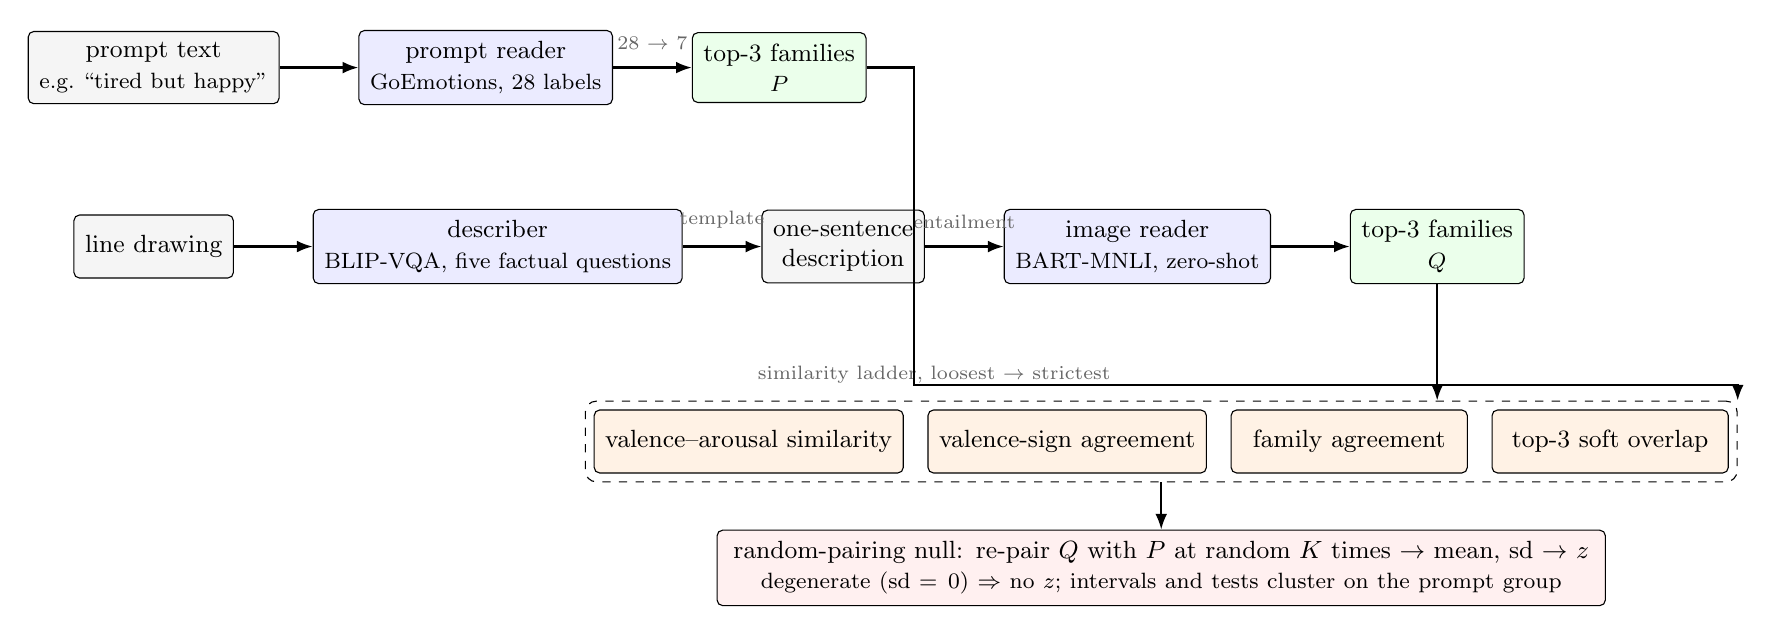
\begin{tikzpicture}[
  font=\small,
  node distance=6mm and 10mm,
  box/.style={draw, rounded corners=2pt, align=center, minimum height=8mm, inner sep=4pt, fill=white},
  data/.style={box, fill=black!4},
  model/.style={box, fill=blue!8},
  res/.style={box, fill=green!8},
  meas/.style={box, fill=orange!10, minimum width=30mm},
  arr/.style={-{Latex[length=2mm]}, thick},
  lab/.style={font=\scriptsize, text=black!60, yshift=1mm}
]
% prompt lane
\node[data] (prompt) {prompt text\\\footnotesize e.g.\ ``tired but happy''};
\node[model, right=of prompt] (goe) {prompt reader\\\footnotesize GoEmotions, 28 labels};
\node[res, right=of goe] (pfam) {top-3 families\\\footnotesize $P$};
\draw[arr] (prompt) -- (goe);
\draw[arr] (goe) -- node[lab, above] {28 $\to$ 7} (pfam);

% image lane
\node[data, below=14mm of prompt] (img) {line drawing};
\node[model, right=of img] (vqa) {describer\\\footnotesize BLIP-VQA, five factual questions};
\node[data, right=of vqa] (desc) {one-sentence\\description};
\node[model, right=of desc] (nli) {image reader\\\footnotesize BART-MNLI, zero-shot};
\node[res, right=of nli] (ifam) {top-3 families\\\footnotesize $Q$};
\draw[arr] (img) -- (vqa);
\draw[arr] (vqa) -- node[lab, above] {template} (desc);
\draw[arr] (desc) -- node[lab, above] {entailment} (nli);
\draw[arr] (nli) -- (ifam);

% ladder
\node[meas, below=16mm of desc, xshift=-12mm] (va) {valence--arousal similarity};
\node[meas, right=3mm of va] (sign) {valence-sign agreement};
\node[meas, right=3mm of sign] (fam) {family agreement};
\node[meas, right=3mm of fam] (ovl) {top-3 soft overlap};
\node[draw, dashed, rounded corners, inner sep=3pt, fit=(va)(sign)(fam)(ovl), label={[lab]above left:similarity ladder, loosest $\to$ strictest}] (ladder) {};
\draw[arr] (pfam.east) -- ++(6mm,0) |- ($(ladder.north east)+(0,2mm)$) -- (ladder.north east);
\draw[arr] (ifam.south) -- (ladder.north -| ifam.south);

% null
\node[box, fill=red!6, below=6mm of ladder, text width=110mm] (null) {random-pairing null: re-pair $Q$ with $P$ at random $K$ times $\to$ mean, sd $\to$ $z$\\\footnotesize degenerate (sd $=0$) $\Rightarrow$ no $z$; intervals and tests cluster on the prompt group};
\draw[arr] (ladder) -- (null);
\end{tikzpicture}
}
\caption{The describe-then-extract pipeline and the similarity ladder. The prompt reader (GoEmotions) and the image reader (BART-MNLI over a BLIP-VQA description) each return a top-3 distribution over seven families; four measures compare them, and each measure is read against the mean and spread it takes when the image readings are re-paired with the prompts at random.}
\label{fig:pipeline}
\end{figure}

\section{The corpus}
\label{sec:method-corpus}
% GUIDANCE: \nTotal\ records (image + prompt text + file timestamp). Collected at Festival of the
% Mind 2024; visitors invited to describe their feeling; the interface accepted any text; one drawing
% per submission. Records are not linked to individuals; \nRepeats\ records repeat an earlier prompt
% (the largest group, "happy", has \nHappy); contributors unknown and no greater than \nDistinct.
% Median prompt length about four words; about 78\% of prompts are entirely lower case (this matters
% for name detection). Generation parameters (model version, seed, any system prompt) were not
% recorded. Figure~\ref{fig:dataset} shows the composition.

\begin{figure}[htbp]
\centering
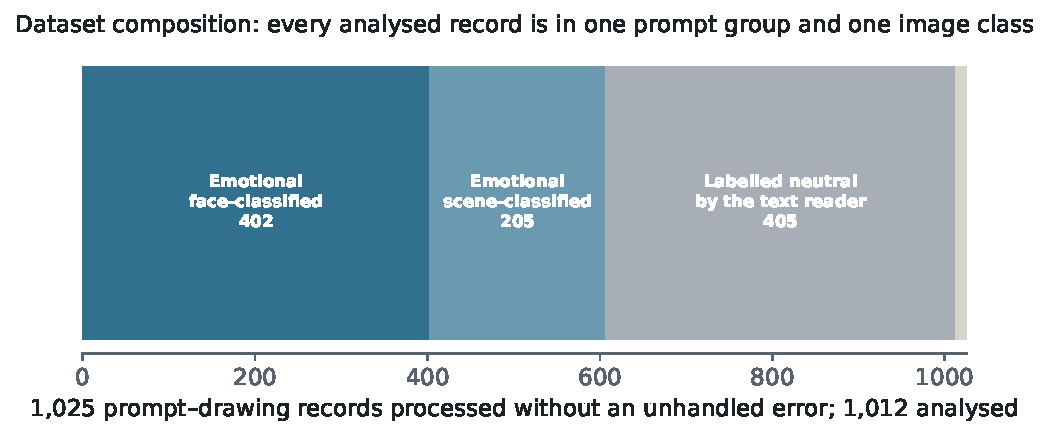
\includegraphics[width=\textwidth]{fig5_dataset}
\caption{Composition of the corpus: \nTotal\ records processed, \nPretest\ pre-festival developer tests excluded, \nAnalysed\ analysed. Every analysed record belongs to exactly one prompt group (emotional / neutral-labelled) and one image class (face-classified / scene-classified); the groups are groupings, not exclusions.}
\label{fig:dataset}
\end{figure}

\section{Data pre-processing}
\label{sec:method-preprocessing}

\subsection{Loading and pre-test removal}
% GUIDANCE: emoviz/data.py unifies three filename schemes and recovers embedded creation timestamps;
% \nPretest\ records with ids 1--13 predate the festival (developer tests) and are excluded from
% analysis but still processed, so the pipeline's completion figure covers all \nTotal.

\subsection{Prompt groups}
% GUIDANCE: dedup\_key is an integer group index computed from the ORIGINAL prompt text (stripped,
% case-folded) BEFORE redaction, so redaction can never merge two different prompts into one group.
% \nDistinct\ groups; \nGroups\ groups hold two or more records (\nGroupRecords\ records). Every
% resampling and permutation in Section~\ref{sec:method-inference} clusters on this key.
% Note the one quirk audits.py found: the key is case-insensitive but the prompt reader saw the
% original case, so a handful of groups mix readings (e.g. "Ok" and "ok"); this does not change any
% count and is reported for completeness.

\subsection{Name redaction}
% GUIDANCE: Describe as data pre-processing, per supervisor direction: names of private individuals
% are replaced by a placeholder at LOAD time; the files on disk are never modified; illness and grief
% content is kept because it is not identifying on its own and is essential to the analysis.
% Three documented stages: DETECT (high recall by design because most prompts are lower case:
% an NLTK given-name gazetteer of 7,944 names \cite{bird2009natural}, mid-sentence capitalisation
% against a 236k-word dictionary, and naming phrases such as "called X"); REVIEW (every candidate
% carries a recorded keep/redact decision with a reason, scoped to the record it was reviewed in, so
% "Jack Frost" and "woolly mammoth" survive; the audit fails if any candidate is unreviewed);
% APPLY (per record). Eight records are affected. Inertness: re-reading the redacted prompts moves
% no GoEmotions probability by more than 0.012 and changes no top-1 family; two records reduce to
% the bare placeholder and are treated separately in the control audit (Section~\ref{sec:method-audits}).
% The decision table travels with the dataset, not with the code.

\section{The pipeline}
\label{sec:method-pipeline}

\subsection{Prompt reader}
% GUIDANCE: GoEmotions \cite{demszky2020goemotions} (SamLowe/roberta-base-go\_emotions, about 125M
% parameters) returns 28 probabilities; they are summed into seven families by the grouping proposed
% with the dataset (Appendix~\ref{app:instruments}), normalised, and the top-3 kept. Rejected: zero-shot
% NLI on the prompts (a third of prompts collapsed to "surprise"); a hand lexicon (the v1 rule).
% An emotional prompt is one whose top-1 family is not neutral (\nEmotional\ of \nAnalysed).

\subsection{Describer}
% GUIDANCE: BLIP-VQA \cite{li2022blip} (Salesforce/blip-vqa-base, about 385M parameters) answers the
% five fixed questions in Appendix~\ref{app:instruments}: facial expression, action, posture, number of
% people, what is in the picture. The word "emotion" appears in none of them. Answers are cached per
% record, which is what makes the ablation possible without re-running the vision model.
% Rejected (with evidence in RESULTS\_describe\_extract.md): a 3B vision--language model that thrashed
% into swap on a 16 GB laptop for 4 h 45 min with zero progress; a plain caption, whose NLI reading
% collapsed to one family.

\subsection{Description template and image reader}
% GUIDANCE: The five answers are composed into one neutral sentence (template in
% Appendix~\ref{app:instruments}); BART-MNLI \cite{lewis2020bart, williams2018broad}
% (facebook/bart-large-mnli, about 407M parameters) scores each family as a hypothesis
% "This scene conveys \{family\}." by entailment \cite{yin2019benchmarking}; the top-3 is kept.
% Say plainly that the template asserts a person and an expression for every drawing, including
% those where the describer reports no people — the consequence is measured in
% Section~\ref{sec:results-describer} and the ablation. Rejected: GoEmotions on the description
% (collapsed to neutral above 0.95).

\subsection{Face and scene classes}
% GUIDANCE: face-classified = the describer reports at least one person AND its expression answer
% contains a word from the documented list in Appendix~\ref{app:instruments} (token match, so
% "man is smiling" counts); scene-classified otherwise. \nFaceAll\ / \nSceneAll\ over all analysed
% records; \nFaceEmo\ / \nSceneEmo\ within the emotional prompts. State the circularity now: the
% class is defined from the same description the image reader reads.

\section{The similarity ladder}
\label{sec:method-measures}
% GUIDANCE: Introduce the notation, then one short paragraph per measure explaining what it rewards
% and what it ignores. Write around the equations; do not restate them in words.

Let each reader return a top-3 list $T = \{(\ell_i, s_i)\}_{i=1}^{3}$ of families $\ell_i \in \mathcal{F}$ with scores $s_i$, where $\mathcal{F} = \{\text{joy}, \text{sadness}, \text{anger}, \text{fear}, \text{surprise}, \text{disgust}, \text{neutral}\}$. Write $P$ for the prompt reader's list and $Q$ for the image reader's, and $\operatorname{top}(T) = \ell_1$ for the top-1 family. Each family has a fixed centroid $c_\ell = (v_\ell, a_\ell)$ on the valence--arousal circumplex (Appendix~\ref{app:instruments}).

\paragraph{Valence--arousal similarity.} The score-weighted centroid of a reading and the similarity between two readings are
\begin{equation}
\mathbf{v}(T) = \frac{\sum_i s_i\, c_{\ell_i}}{\sum_i s_i}, \qquad
S_{\mathrm{VA}}(P, Q) = 1 - \frac{1}{\sqrt{2}}\,\Bigl\|\Bigl(\tfrac{v_P + 1}{2} - \tfrac{v_Q + 1}{2},\; a_P - a_Q\Bigr)\Bigr\|_2 ,
\label{eq:va}
\end{equation}
where $(v_P, a_P) = \mathbf{v}(P)$ and likewise for $Q$. Valence is rescaled to $[0,1]$ so both axes have unit range. Over the seven centroids the smallest attainable value is $0.412$ (joy against sadness), and randomly paired records average about \FullNeuVaNull; this floor is why the measure is never quoted without its null.

\paragraph{Top-3 soft overlap.} Each side is first normalised to a distribution over its own three families, $\tilde{p}_\ell = s_\ell / \sum_j s_j$, so the prompt reader's multi-label scale and the image reader's softmax scale are comparable; the overlap is the sum of per-family minima,
\begin{equation}
S_{\mathrm{ovl}}(P, Q) = \sum_{\ell \in \mathcal{F}} \min\bigl(\tilde{p}_\ell,\; \tilde{q}_\ell\bigr) \in [0, 1],
\label{eq:overlap}
\end{equation}
which equals one only when the two distributions coincide.

\paragraph{Family agreement.} Over a set of $n$ records,
\begin{equation}
A_{\mathrm{fam}} = \frac{1}{n} \sum_{i=1}^{n} \mathbb{1}\bigl[\operatorname{top}(P_i) = \operatorname{top}(Q_i)\bigr].
\label{eq:family}
\end{equation}

\paragraph{Valence-sign agreement.} With $\sigma(\ell) \in \{+, -, 0\}$ the sign of a family ($+$ for joy; $-$ for sadness, anger, fear, disgust; $0$ for surprise and neutral),
\begin{equation}
A_{\mathrm{sign}} = \frac{\sum_{i} \mathbb{1}\bigl[\sigma(\operatorname{top} P_i) \neq 0 \;\wedge\; \sigma(\operatorname{top} P_i) = \sigma(\operatorname{top} Q_i)\bigr]}{\sum_{i} \mathbb{1}\bigl[\sigma(\operatorname{top} P_i) \neq 0\bigr]} ,
\label{eq:sign}
\end{equation}
so records whose prompt family has no sign are excluded from the denominator; the denominator is reported with every value (for example \FullEmoNSign\ of the \FullEmoN\ emotional prompts).

\section{The random-pairing null}
\label{sec:method-null}
% GUIDANCE: Why a null: the measures do not start at zero (Eq.~\ref{eq:va}'s floor; the family
% marginals in Table~\ref{tab:families} make "joy" agreement likely by chance). The null is the
% exchangeability hypothesis that the image reading is unrelated to the prompt \cite{good2005permutation}.
% Note that with K = \nullShuffles\ re-pairings the null sd is itself an estimate: across seeds 1--5 the
% headline z moves between \ZSeedMin\ and \ZSeedMax, so z orders effects, it is not a precise
% probability. Then degenerate nulls, detected automatically from the null's spread.

For a subset of $n$ records and a measure $m$, draw $K$ random permutations $\pi_k$ of the image readings and compute $m_k = m\bigl(\{(P_i, Q_{\pi_k(i)})\}_{i=1}^{n}\bigr)$. With $\hat\mu = \frac{1}{K}\sum_k m_k$ and $\hat\sigma$ the standard deviation of $\{m_k\}$,
\begin{equation}
z = \frac{m_{\mathrm{obs}} - \hat\mu}{\hat\sigma}, \qquad K = \nullShuffles,\ \text{seed}\ \nullSeed .
\label{eq:z}
\end{equation}
A null is \emph{degenerate} when $\hat\sigma = 0$: this happens for family agreement when every prompt in the subset shares one top-1 family, and for valence-sign agreement when every prompt shares one sign, because permuting the image side then cannot change the score. The analysis detects this from the null itself and prints no $z$ for such cells.

\section{Inference}
\label{sec:method-inference}
% GUIDANCE: Explain why records are not independent (\nRepeats\ repeats) and that every interval and
% test therefore clusters on the prompt group \cite{cameron2008bootstrap}. One paragraph each.

\paragraph{Clustered bootstrap confidence intervals.} Let $\mathcal{G}$ be the set of prompt groups in a subset. For $b = 1, \dots, B$ draw $|\mathcal{G}|$ groups with replacement, pool their records, and recompute the measure; the 95\% interval is the 2.5th and 97.5th percentiles of the $B$ values \cite{efron1993introduction}, with $B = \DiffDraws$ and seed \nullSeed.

\paragraph{Clustered permutation test of the face/scene difference.} Under the null that the image class is unrelated to agreement, the face/scene labels are exchangeable across prompt groups. The labels are permuted across groups $P$ times and the difference in agreement recomputed; the two-sided $p$-value uses the estimator of \cite{north2002note},
\begin{equation}
p = \frac{k + 1}{P + 1}, \qquad k = \#\{\text{permuted differences at least as extreme as the observed}\},
\label{eq:permp}
\end{equation}
so the smallest reportable value with $P = \DiffDraws$ is $10^{-4}$.

\paragraph{Cohen's kappa.} For comparability with other studies, family agreement is also reported as
\begin{equation}
\kappa = \frac{p_o - p_e}{1 - p_e},
\label{eq:kappa}
\end{equation}
with $p_o$ the observed top-1 agreement and $p_e$ the agreement expected from the two readers' family marginals \cite{cohen1960coefficient}, interpreted with the bands of \cite{landis1977measurement}; intervals by the clustered bootstrap above.

\paragraph{Multiple comparisons.} The analysis prints \HolmM\ non-degenerate $z$-scores. Each is converted to a two-sided $p$ by the normal approximation and the family is controlled with the Holm--Bonferroni step-down procedure \cite{holm1979simple}: order $p_{(1)} \le \dots \le p_{(m)}$ and reject while $p_{(i)} \le \alpha / (m - i + 1)$, $\alpha = 0.05$.

\paragraph{Paired comparison of two image readers.} On the same records each reader either agrees with the prompt reader or does not. With $b$ the records only the first reader agrees on and $c$ only the second, McNemar's exact binomial test \cite{mcnemar1947note} on $(b, c)$ treats records as independent and is therefore optimistic here; the clustered version flips the sign of each prompt group's summed difference as a block (\McClusterDraws\ draws) and the clustered bootstrap gives the interval on the difference in rates.

\paragraph{Wilson intervals.} Proportions from the single-coder check use the Wilson score interval \cite{wilson1927probable}, which behaves at small $n$ and near 0 and 1.

\section{Analyses}
\label{sec:method-analyses}
% GUIDANCE: One paragraph per analysis, in the order the results are reported. Name the script.
%   Splits (analysis\_final.py): emotional / neutral-labelled prompts; face / scene within emotional;
%     positive / negative valence (VA only, the others are degenerate); all against the null of Eq.~\ref{eq:z}.
%   Distinct-prompt robustness: the same table on the first occurrence of each prompt (\nDistinct\ records).
%   Face/scene difference (significance.py): clustered bootstrap CI and clustered permutation test.
%   Specificity check: neutral-labelled prompts should sit at their null; only VA is informative there.
%   Method comparison (method\_comparison.py): the SAME prompt reader, subset, measures and re-pairings,
%     varying only the image reader (describe-then-extract vs direct CLIP zero-shot \cite{radford2021learning,
%     ilharco2021openclip}); paired tests as above. State that the earlier v1 comparison used a different
%     prompt reader, subset and overlap formula and is kept only as a record (Table~\ref{tab:methodvone}).
%   Consistency (data\_audit\_consistency.py): defined below, with its permutation null.
%   Control audit (audits.py): a fixed \CtrlLexicon-word affect lexicon over the \CtrlN\ neutral-labelled
%     prompts; the two placeholder-only records; the specificity check re-run on the cleaned control.
%   Describer audit (audits.py): people count crossed with expression word; the copy rate defined below.
%   Error taxonomy (error\_taxonomy.py): every emotional record where both readers score at least 0.8 and
%     disagree on family, each drawing inspected and assigned one of six failure modes.
%   Ablation (ablate\_nli.py): rebuild each description from the cached answers with one clause removed
%     (expression, action, posture, people, scene) or the expression fixed to "unclear"; re-run only the
%     NLI stage; recompute the ladder and nulls with identical code.
%   Human check (human\_check.py): a fixed, stratified 120-drawing sample coded by one coder blind to
%     prompt and model output for person present, readable face, valence and family; describer and reader
%     scored against the codes with Wilson intervals; the face/scene contrast re-run on the coder's split.

\paragraph{Consistency across repeated prompts.} For a prompt group $g$ with $n_g \ge 2$ records and image top-1 families $\{\operatorname{top}(Q_i)\}_{i \in g}$, the modal fraction is $c_g = \max_{\ell} n_{g,\ell} / n_g$, and the consistency is the mean $C = \frac{1}{|\mathcal{G}_{\ge 2}|} \sum_g c_g$ over the \nGroups\ groups. Because \nPairGroups\ groups are pairs, $c_g$ cannot fall below $0.5$ for them, so $C$ is read against a permutation null that shuffles the image top-1 families across all \nAnalysed\ analysed records and re-cuts them into the same groups (\ConsDraws\ draws). The count of fully consistent groups ($c_g = 1$) is treated the same way. This bounds the reproducibility of the whole prompt-to-reading chain; it does not isolate the generator, whose parameters were not recorded.

\paragraph{Copy rate.} Where the describer's expression answer is a single word that names an emotion (strict: happy, sad, angry, \dots; \DescBareStrictN\ records) or a facial action with an implied family (broad: smile, crying, \dots; \DescBareBroadN\ records), the copy rate is the share of those records in which the image reader's top-1 family equals the family the word implies. It measures how much the "separate" extraction stage adds beyond the describer's own word.

\section{The demonstrator}
\label{sec:method-demo}
% GUIDANCE: A local Flask application that runs the real pipeline on any of the \nAnalysed\ records
% or an uploaded image, shows the five answers and the description, both readings, and the ladder
% against the SAME null as the analysis (computed at start-up from the same result files). Design
% choices to state: the valence--arousal axis starts at its floor and shades the middle half of random
% pairings; the verdict leads with valence sign and family; nothing a visitor types or uploads is
% stored. It is a testing and communication tool, not a data-collection tool.

\section{Reproducibility and testing}
\label{sec:method-repro}
% GUIDANCE: Pinned environment (requirements.txt), seeded randomness, cached model outputs so every
% analysis re-runs in seconds, a frozen direct-CLIP baseline file, and one metrics module shared by
% every script so definitions cannot drift. Two layers of tests: test.sh (smoke checks — environment,
% data integrity, every script exits 0, a live three-image pipeline run, the redaction audit) and
% test\_numeric.py (every headline value pinned to the JSON that produces it, plus unit tests of the
% measures: the 0.412 floor, symmetry, overlap bounds). Figures and every number in this document are
% generated from the same JSON (make\_figures.py, export\_tex.py). Say what the tests do NOT do: none
% validates a model answer against a human label — that is what the human check is for.
% Appendix~\ref{app:repro} lists the files and the run order.
   % Methodology
\chapter{Results}
\label{ch:results}

This chapter reports what the analyses found. Interpretation is held back for Chapter~\ref{ch:discussion}; here the tables and figures carry the numbers and the prose says what each shows. Every value is a macro generated from the result files, every rate is read against its random-pairing null (\nullShuffles{} re-pairings, seed \nullSeed), and every interval is a clustered bootstrap over prompt groups (\DiffDraws{} draws).

\section{Overall agreement}
\label{sec:results-overall}

Table~\ref{tab:headline} gives the four measures on the \nEmotional{} prompts the text reader labels emotional, and Figure~\ref{fig:zgroup} shows the same cells as distances from their nulls. Every measure sits well above chance. Valence-sign agreement is \FullEmoSignObs{} against a null of \FullEmoSignNull{} ($z$ = \FullEmoSignZ{}, 95\% CI \FullEmoSignCi{}); the denominator is \FullEmoNSign{} rather than \FullEmoN{}, because prompts whose top family is surprise have no valence sign. Family agreement is \FullEmoFamObs{} against \FullEmoFamNull{} ($z$ = \FullEmoFamZ{}, CI \FullEmoFamCi{}), top-3 overlap \FullEmoOvlpObs{} against \FullEmoOvlpNull{} ($z$ = \FullEmoOvlpZ{}), and valence--arousal similarity \FullEmoVaObs{} against \FullEmoVaNull{} ($z$ = \FullEmoVaZ{}). The loosest measure has the largest $z$ and the smallest gap in percentage points, which is the floor of Equation~\ref{eq:va} at work: its null is high and tight, so a modest excess over it is many standard deviations.

% GENERATED by emoviz/export_tex.py — do not edit
\begin{table}[htbp]
\centering
\small
\caption{Agreement between the prompt reader and the image reader on the 1,012 analysed records, by prompt group and image class, against the random-pairing null (300 re-pairings, seed 7). CI: clustered bootstrap over prompt groups (10,000 draws). n/a: degenerate null (every prompt in the subset shares one label, so permutation cannot change the score).}
\label{tab:headline}
\begin{tabular}{lrrrl}
\toprule
Subset / measure & Observed & Null & $z$ & 95\% CI \\
\midrule
\textbf{Emotional prompts} ($n$=607; sign $n$=530) &  &  &  &  \\
Valence--arousal similarity & 83.8\% & 77.3\% & +12.2 & [82.0, 85.5] \\
Valence-sign agreement & 64.0\% & 45.6\% & +11.1 & [58.6, 68.8] \\
Family agreement & 53.0\% & 38.8\% & +10.3 & [47.3, 58.7] \\
Top-3 soft overlap & 50.6\% & 39.4\% & +11.6 & [46.5, 54.7] \\
\midrule
\textbf{\quad face-classified} ($n$=402; sign $n$=360) &  &  &  &  \\
Valence--arousal similarity & 84.2\% & 76.4\% & +11.2 & [82.3, 86.1] \\
Valence-sign agreement & 73.9\% & 53.5\% & +10.4 & [68.3, 79.2] \\
Family agreement & 61.9\% & 45.8\% & +10.3 & [55.8, 68.0] \\
Top-3 soft overlap & 53.4\% & 40.4\% & +11.6 & [49.2, 57.7] \\
\midrule
\textbf{\quad scene-classified} ($n$=205; sign $n$=170) &  &  &  &  \\
Valence--arousal similarity & 82.9\% & 79.1\% & +6.0 & [80.4, 85.2] \\
Valence-sign agreement & 42.9\% & 29.6\% & +5.8 & [33.1, 51.1] \\
Family agreement & 35.6\% & 26.2\% & +4.4 & [26.4, 44.1] \\
Top-3 soft overlap & 44.9\% & 38.1\% & +4.9 & [38.7, 51.0] \\
\midrule
\textbf{Neutral-labelled prompts} ($n$=405; sign $n$=0) &  &  &  &  \\
Valence--arousal similarity & 76.6\% & 76.6\% & +0.3 & [75.6, 77.6] \\
Valence-sign agreement & 0.0\% & 0.0\% & n/a & degenerate \\
Family agreement & 28.6\% & 28.6\% & n/a & degenerate \\
Top-3 soft overlap & 31.6\% & 31.6\% & +0.0 & -- \\
\bottomrule
\end{tabular}
\end{table}


\begin{figure}[htbp]
\centering
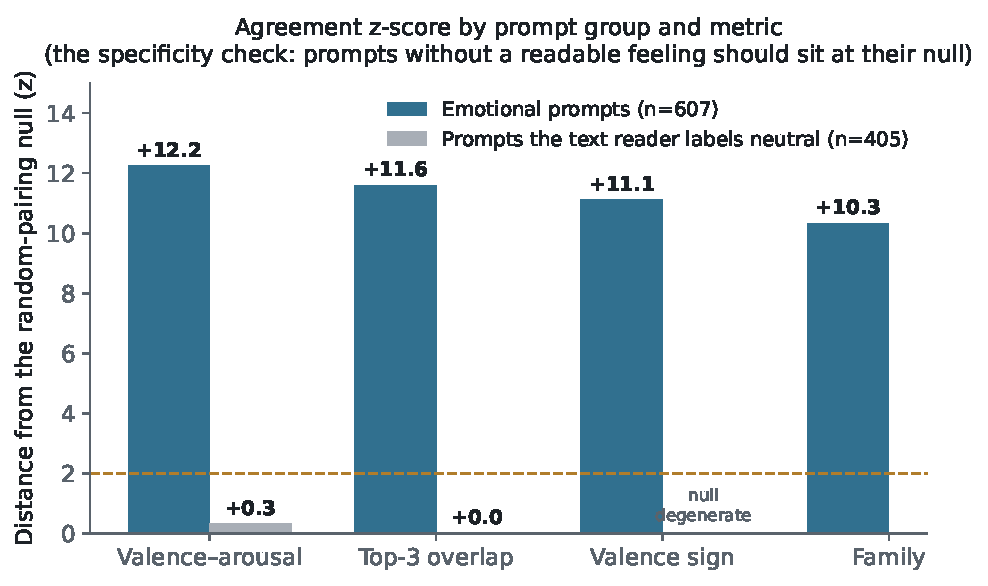
\includegraphics[width=0.9\textwidth]{fig3_z_by_prompt_group}
\caption{Distance from the random-pairing null ($z$) by prompt group and measure. For the neutral-labelled prompts the sign and family nulls are degenerate and no $z$ is shown.}
\label{fig:zgroup}
\end{figure}

\section{Face-classified versus scene-classified drawings}
\label{sec:results-face-scene}

Figure~\ref{fig:facescene} and Table~\ref{tab:difference} split the emotional prompts by the describer's image class. On the \FullFaceN{} face-classified records valence-sign agreement is \FullFaceSignObs{} against a null of \FullFaceSignNull{} ($z$ = \FullFaceSignZ{}, CI \FullFaceSignCi{}) and family agreement \FullFaceFamObs{} against \FullFaceFamNull{} ($z$ = \FullFaceFamZ{}). On the \FullSceneN{} scene-classified records the same measures are \FullSceneSignObs{} against \FullSceneSignNull{} ($z$ = \FullSceneSignZ{}, CI \FullSceneSignCi{}) and \FullSceneFamObs{} against \FullSceneFamNull{} ($z$ = \FullSceneFamZ{}). Both classes clear their nulls in this table; Section~\ref{sec:results-ablation} returns to the scene row.

The two nulls differ, so the contrast is stated as a difference rather than a ratio. Face minus scene is \DiffSignPp{} on valence-sign agreement (CI \DiffSignCi{}) and \DiffFamPp{} on family agreement (CI \DiffFamCi{}), with the clustered permutation test giving $p$ = \DiffSignP{} on both. Valence--arousal similarity does not separate the classes (\FullFaceVaObs{} against \FullSceneVaObs{}); the difference lives in the categorical rungs.

\begin{figure}[htbp]
\centering
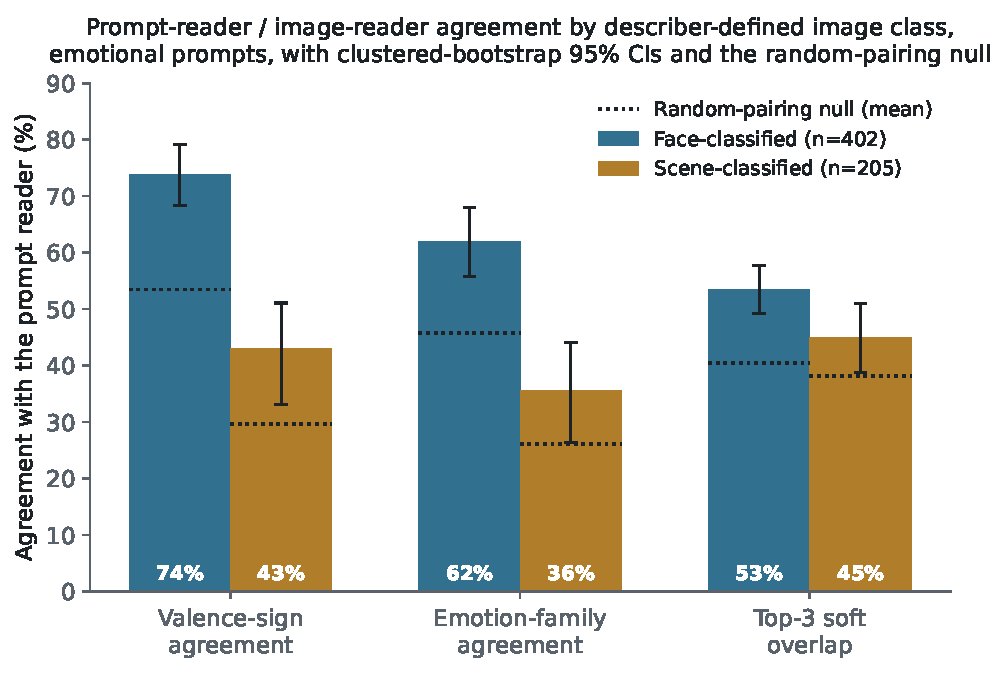
\includegraphics[width=\textwidth]{fig1_face_vs_scene}
\caption{Agreement between the prompt reader and the image reader on the emotional prompts, by describer-defined image class, with clustered-bootstrap 95\% CIs (error bars) and each cell's random-pairing null (dotted).}
\label{fig:facescene}
\end{figure}

% GENERATED by emoviz/export_tex.py — do not edit
\begin{table}[htbp]
\centering
\footnotesize
\caption{Face-classified versus scene-classified drawings on the emotional prompts: agreement with 95\% clustered-bootstrap CIs, the difference with its CI, and the clustered permutation p (10,000 draws; significance.py).}
\label{tab:difference}
\begin{tabular}{lllll}
\toprule
Measure & Face ($n$=402) & Scene ($n$=205) & Difference (pp) & Perm.\ $p$ \\
\midrule
Valence-sign agreement & 73.9\% [68.3, 79.2] & 42.9\% [33.1, 51.1] & +30.9~pp [+22.6, +40.6] & 0.0001 \\
Family agreement & 61.9\% [55.8, 68.0] & 35.6\% [26.4, 44.1] & +26.3~pp [+18.4, +35.3] & 0.0001 \\
\bottomrule
\end{tabular}
\end{table}


\section{Robustness to repeated prompts and multiple comparisons}
\label{sec:results-robustness}

Table~\ref{tab:distinct} recomputes the main table on the first occurrence of each prompt, \nDistinct{} records of which \nDistinctEmo{} are emotional. The overall and face results hold: on the \DistFaceN{} distinct face-classified records valence-sign agreement is \DistFaceSignObs{} ($z$ = \DistFaceSignZ{}) and family agreement \DistFaceFamObs{} ($z$ = \DistFaceFamZ{}). The scene result weakens substantially: valence-sign agreement falls to \DistSceneSignObs{} ($z$ = \DistSceneSignZ{}) and family agreement to \DistSceneFamObs{} ($z$ = \DistSceneFamZ{}) on \DistSceneN{} records.

Table~\ref{tab:holm} applies the Holm--Bonferroni procedure to the \HolmM{} non-degenerate $z$-scores the analysis prints. \HolmSurvive{} survive at family-wise 0.05 and \HolmFail{} do not. Every full-sample cell on the emotional, face and scene subsets survives, as does every distinct-prompt cell on the emotional and face subsets. The cells that fail are the ones expected to sit at chance (the neutral-labelled control on both blocks), the single-valence subsets' valence--arousal and overlap cells, and the distinct-prompt scene family cell ($z$ = \DistSceneFamZ{}), which should be read as suggestive rather than established.

% GENERATED by emoviz/export_tex.py — do not edit
\begin{table}[htbp]
\centering
\small
\caption{The same analysis on the 763 distinct prompts only (first occurrence of each prompt text kept), a check against pseudo-replication from the 249 repeated prompts.}
\label{tab:distinct}
\begin{tabular}{lrrrl}
\toprule
Subset / measure & Observed & Null & $z$ & 95\% CI \\
\midrule
\textbf{Emotional prompts} ($n$=452; sign $n$=394) &  &  &  &  \\
Valence--arousal similarity & 83.0\% & 76.5\% & +10.6 & [81.5, 84.4] \\
Valence-sign agreement & 62.2\% & 44.4\% & +9.9 & [57.2, 67.0] \\
Family agreement & 51.3\% & 37.2\% & +9.3 & [46.7, 56.0] \\
Top-3 soft overlap & 48.9\% & 37.7\% & +10.8 & [45.9, 51.9] \\
\midrule
\textbf{\quad face-classified} ($n$=319; sign $n$=284) &  &  &  &  \\
Valence--arousal similarity & 83.5\% & 75.5\% & +9.7 & [81.7, 85.2] \\
Valence-sign agreement & 71.8\% & 51.0\% & +8.4 & [66.4, 77.0] \\
Family agreement & 59.9\% & 43.0\% & +8.1 & [54.2, 65.2] \\
Top-3 soft overlap & 51.8\% & 38.4\% & +9.7 & [48.1, 55.4] \\
\midrule
\textbf{\quad scene-classified} ($n$=133; sign $n$=110) &  &  &  &  \\
Valence--arousal similarity & 81.8\% & 78.9\% & +3.6 & [79.5, 83.8] \\
Valence-sign agreement & 37.3\% & 27.1\% & +3.5 & [28.1, 46.2] \\
Family agreement & 30.8\% & 24.1\% & +2.6 & [23.3, 38.4] \\
Top-3 soft overlap & 41.7\% & 36.7\% & +3.1 & [36.9, 46.5] \\
\midrule
\textbf{Neutral-labelled prompts} ($n$=311; sign $n$=0) &  &  &  &  \\
Valence--arousal similarity & 76.6\% & 76.4\% & +1.1 & -- \\
Valence-sign agreement & 0.0\% & 0.0\% & n/a & degenerate \\
Family agreement & 27.7\% & 27.7\% & n/a & degenerate \\
Top-3 soft overlap & 31.4\% & 31.1\% & +0.8 & -- \\
\bottomrule
\end{tabular}
\end{table}

% GENERATED by emoviz/export_tex.py — do not edit
\begin{table}[htbp]
\centering
\footnotesize
\caption{Multiple-comparison control over the 36 non-degenerate $z$-scores the analysis prints (12 degenerate ones excluded). Two-sided $p$ by the normal approximation; Holm--Bonferroni at family-wise 0.05: 26 survive, 10 do not.}
\label{tab:holm}
\begin{tabular}{lp{0.78\textwidth}}
\toprule
Outcome & Tests \\
\midrule
Do not survive & DISTINCT negative prompts overlap z+2.7; DISTINCT scene images family z+2.6; FULL positive prompts overlap z+2.3; FULL negative prompts va z+2.1; DISTINCT positive prompts overlap z+1.9; DISTINCT negative prompts va z+1.6; DISTINCT non-emotional va z+1.1; DISTINCT non-emotional overlap z+0.8; FULL non-emotional va z+0.3; FULL non-emotional overlap z+0.0 \\
Survive & the remaining 26, including every headline (emotional, face and scene on all four measures; distinct-prompt emotional and face) \\
\bottomrule
\end{tabular}
\end{table}


\section{Specificity check: prompts the text reader labels neutral}
\label{sec:results-control}

On the \CtrlN{} prompts the text reader labels neutral, only the valence--arousal measure has a live null. It sits on it: \CtrlVaObs{} observed against \CtrlVaNull{} expected ($z$ = \CtrlVaZ{} at record level, \CtrlVaZClustered{} against a null clustered on prompt groups). Family agreement equals its null exactly (\CtrlFamObs{}) because every prompt in the subset shares the neutral label, so permutation cannot move it; the same holds for valence sign, whose numerator and denominator are both zero here.

The control audit (Table~\ref{tab:control}) qualifies the set. \CtrlFlagged{} of the \CtrlN{} prompts (\CtrlFlaggedPct{}) contain a plain English affect word from a fixed \CtrlLexicon{}-word lexicon, most often \CtrlTopWords{}; \CtrlNameOnly{} consist of a redacted name alone. On the cleaned control of \CtrlCleanN{} records the result is unchanged: \CtrlCleanVaObs{} against \CtrlCleanVaNull{} ($z$ = \CtrlCleanVaZ{}). The null's spread on this subset is very small (\CtrlVaSd{}) because the prompt-side points barely vary, so observed and expected values are expected to coincide here; the check is passed, and it is a weak one.

% GENERATED by emoviz/export_tex.py — do not edit
\begin{table}[htbp]
\centering
\small
\caption{The specificity check on the prompts the text reader labels neutral. Only valence--arousal similarity is informative there (sign and family are degenerate: every prompt shares the neutral label). Cleaned control = minus the 2 records reduced to `[name]' and the 68 containing one of 66 plain affect words.}
\label{tab:control}
\begin{tabular}{lrrrrr}
\toprule
Control set & $n$ & VA observed & VA null & $z$ (record null) & $z$ (clustered null) \\
\midrule
All neutral-labelled prompts & 405 & 76.6\% & 76.5\% & +0.5 & -0.1 \\
Cleaned control & 335 & 76.6\% & 76.6\% & +0.0 & -0.6 \\
\bottomrule
\end{tabular}
\end{table}


\section{Two image readers, like for like}
\label{sec:results-method}

Figure~\ref{fig:method} and Table~\ref{tab:method} score two image readers against the same prompt reader on the same \McN{} emotional records with the same measures and the same random re-pairings. Describe-then-extract agrees with the prompt reader on \McDeFam{} of families against \McClipFam{} for direct CLIP, a difference of \McDiffFamPp{} (CI \McDiffFamCi{}); the cluster sign-flip test gives $p$ \McClusterFamP{}, and the unclustered exact McNemar test, which treats records as independent and is optimistic, gives $p$ = \McMcNemarFamP{}. On valence sign the figures are \McDeSign{} against \McClipSign{} (\McDiffSignPp{}, CI \McDiffSignCi{}); on overlap \McDeOvlp{} against \McClipOvlp{}; on valence--arousal similarity \McDeVa{} against \McClipVa{}. Of the \McN{} records, \McFamB{} are ones only describe-then-extract agrees on and \McFamC{} ones only direct CLIP agrees on; \McFamBoth{} are agreed by both and \McFamNeither{} by neither.

Two details in the table need saying. Direct CLIP's family $z$ (\McClipFamZ{}) is higher than describe-then-extract's (\McDeFamZ{}) although its rate is far lower, because its null is lower and tighter: it reads \McClipNeutral{} of the \McN{} images as neutral, so it rarely agrees by chance either. The $z$ measures distance from chance, not level of agreement, and the paired tests on the rates are the comparison. And the two image readers agree with each other on only \McReaderAgree{} of top-1 families. Table~\ref{tab:methodvone} reproduces the comparison from the first build (\McVOneN{} records, an entailment reader on the prompt side, a different overlap formula), kept as a record; it is not comparable with the main analysis and its figures are not quoted.

\begin{figure}[htbp]
\centering
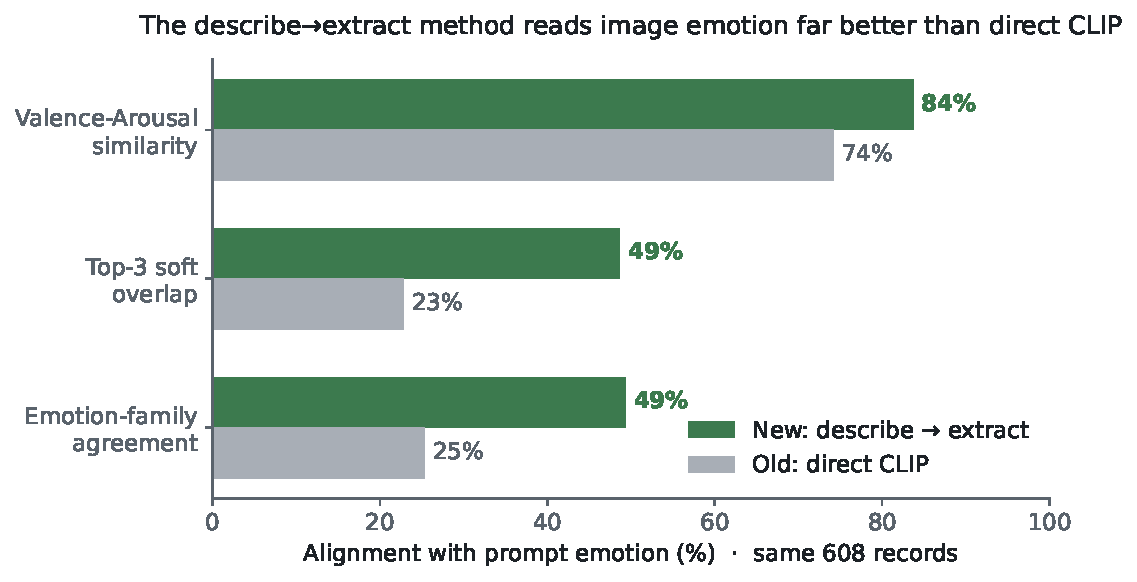
\includegraphics[width=\textwidth]{fig2_method_comparison}
\caption{Two image readers scored against the same prompt reader on the same \McN{} emotional records, each against its own random-pairing null (dotted).}
\label{fig:method}
\end{figure}

% GENERATED by emoviz/export_tex.py — do not edit
\begin{table}[htbp]
\centering
\scriptsize
\caption{Two image readers scored like for like against the same prompt reader (GoEmotions) on the same 607 emotional records with the same measures and the same 300 re-pairings. $b$ = records only describe-then-extract agrees on; $c$ = records only direct CLIP agrees on. The exact McNemar $p$ treats records as independent and is optimistic ($3.4\times10^{-35}$ for family); the cluster sign-flip randomisation (20,000 draws) respects prompt groups.}
\label{tab:method}
\begin{tabular}{lrrrrrr}
\toprule
Measure & Describe→extract & null & $z$ & Direct CLIP & null & $z$ \\
\midrule
Valence--arousal similarity & 83.8\% & 77.3\% & +12.2 & 73.3\% & 70.1\% & +10.2 \\
Valence-sign agreement & 64.0\% & 45.6\% & +11.1 & 31.1\% & 18.6\% & +9.9 \\
Family agreement & 53.0\% & 38.8\% & +10.3 & 22.4\% & 12.2\% & +11.1 \\
Top-3 soft overlap & 50.6\% & 39.4\% & +11.6 & 26.4\% & 20.2\% & +11.2 \\
\midrule
Paired family test & $b$=218, $c$=32 &  &  & diff +30.6~pp & CI [+25.5, +35.6] & cluster $p<0.001$ \\
Paired valence-sign test & $b$=204, $c$=30 &  &  & diff +32.8~pp & CI [+27.4, +38.2] & cluster $p<0.001$ \\
\bottomrule
\end{tabular}
\end{table}

% GENERATED by emoviz/export_tex.py — do not edit
\begin{table}[htbp]
\centering
\small
\caption{The earlier (v1) comparison as published in the build log: prompt side read by BART-MNLI, the 608 records of the v1 lexicon rule, and a different overlap formula. Kept as a record; not comparable with Table~\ref{tab:headline}.}
\label{tab:methodvone}
\begin{tabular}{lrr}
\toprule
Measure & Describe→extract & Direct CLIP \\
\midrule
Family agreement & 49.3\% & 25.3\% \\
Top-3 soft overlap & 48.6\% & 22.8\% \\
Valence--arousal similarity & 83.7\% & 74.2\% \\
\bottomrule
\end{tabular}
\end{table}


\section{Consistency across repeated prompts}
\label{sec:results-consistency}

\nGroups{} prompts were drawn two or more times, covering \nGroupRecords{} records; \nPairGroups{} of the groups are pairs. Figure~\ref{fig:consistency} and Table~\ref{tab:consistency} give the within-group agreement of the image reader. The mean share of drawings in a group that receive the group's modal family is \ConsFam{} (CI over groups \ConsFamCi{}) against a permutation null of \ConsFamNull{} (sd \ConsFamNullSd{}), $z$ = \ConsFamZ{}, permutation $p$ = \ConsFamP{}. The same valence sign is returned for \ConsVal{} of drawings within a group against \ConsValNull{} ($z$ = \ConsValZ{}). \ConsFull{} of the \nGroups{} groups (\ConsFullPct{}) are fully consistent, every drawing receiving one family, against \ConsFullNull{} expected ($z$ = \ConsFullZ{}). The largest group, the word ``happy'' drawn \ConsHappyN{} times, was read as joy \ConsHappyJoy{} times, neutral \ConsHappyNeutral{} times and surprise \ConsHappySurprise{} once.

\begin{figure}[htbp]
\centering
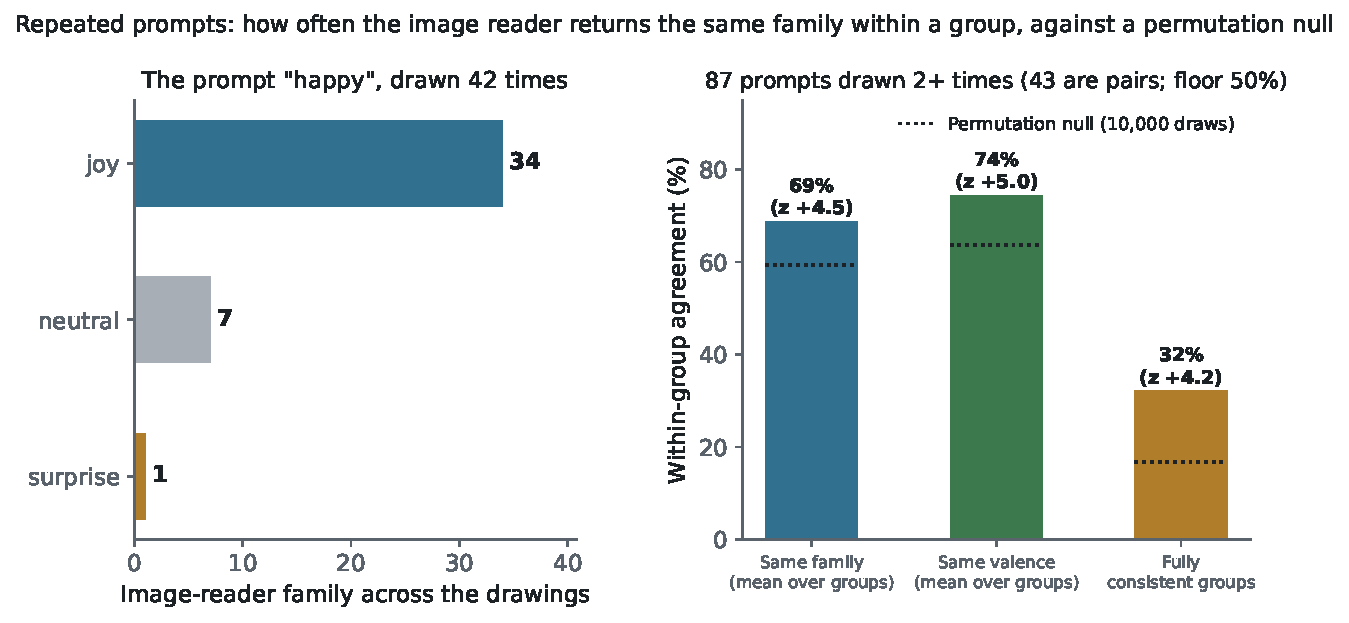
\includegraphics[width=\textwidth]{fig4_consistency}
\caption{Repeated prompts: the image reader's top-1 family across the \ConsHappyN{} drawings of ``happy'' (left), and within-group agreement over all \nGroups{} repeated prompts against the permutation null (right).}
\label{fig:consistency}
\end{figure}

% GENERATED by emoviz/export_tex.py — do not edit
\begin{table}[htbp]
\centering
\small
\caption{Within-group agreement of the image reader across the 87 prompts drawn two or more times (336 records; 43 groups are pairs, whose modal agreement cannot fall below 50\%), against a permutation null that shuffles the image readings over all 1,012 analysed records and re-cuts them into the same groups (10,000 draws, seed 7).}
\label{tab:consistency}
\begin{tabular}{lrrrr}
\toprule
Quantity & Observed & Null mean (sd) & $z$ & $p$ \\
\midrule
Same family, mean over groups & 68.8\% & 59.4\% (2.1\%) & +4.5 & $1.0\times10^{-4}$ \\
Same valence, mean over groups & 74.5\% & 63.7\% (2.1\%) & +5.0 & $1.0\times10^{-4}$ \\
Fully consistent groups (of 87) & 28 & 14.5 (3.2) & +4.2 & $2.0\times10^{-4}$ \\
\bottomrule
\end{tabular}
\end{table}


\section{Per-family agreement}
\label{sec:results-families}

Figure~\ref{fig:confusion} and Table~\ref{tab:confusion} cross the prompt reader's family with the image reader's on the \nEmotional{} emotional records; Table~\ref{tab:families} gives the marginals over all \nAnalysed{} analysed records. The prompt side is dominated by joy (\RecJoyN{} of the emotional prompts), with sadness (\RecSadnessN{}) and surprise (\RecSurpriseN{}) next and fear (\RecFearN{}), anger (\RecAngerN{}) and disgust (\RecDisgustN{}) rare. Recall by prompt family, meaning the share of prompts in a family whose drawing the image reader placed in the same family, is \RecJoy{} for joy (CI \RecJoyCi{}), \RecSadness{} for sadness (CI \RecSadnessCi{}), \RecAnger{} for anger on \RecAngerN{} prompts, \RecSurprise{} for surprise (CI \RecSurpriseCi{}), and \RecFear{} for fear on \RecFearN{} prompts. Across all \nAnalysed{} records the image reader never returns disgust and returns fear \famImageFear{} times.

Cohen's kappa for family agreement (Table~\ref{tab:kappa}) is \KappaEmo{} on the emotional prompts (CI \KappaEmoCi{}), \KappaFace{} on the face-classified records and \KappaScene{} on the scene-classified: \KappaEmoBand{}, \KappaFaceBand{} and \KappaSceneBand{} on the Landis--Koch scale. In practice the seven-family ladder is a three-family one, joy, sadness and neutral, with anger a distant fourth; the remaining families are too rare on the prompt side, or never produced on the image side, to support any claim.

\begin{figure}[htbp]
\centering
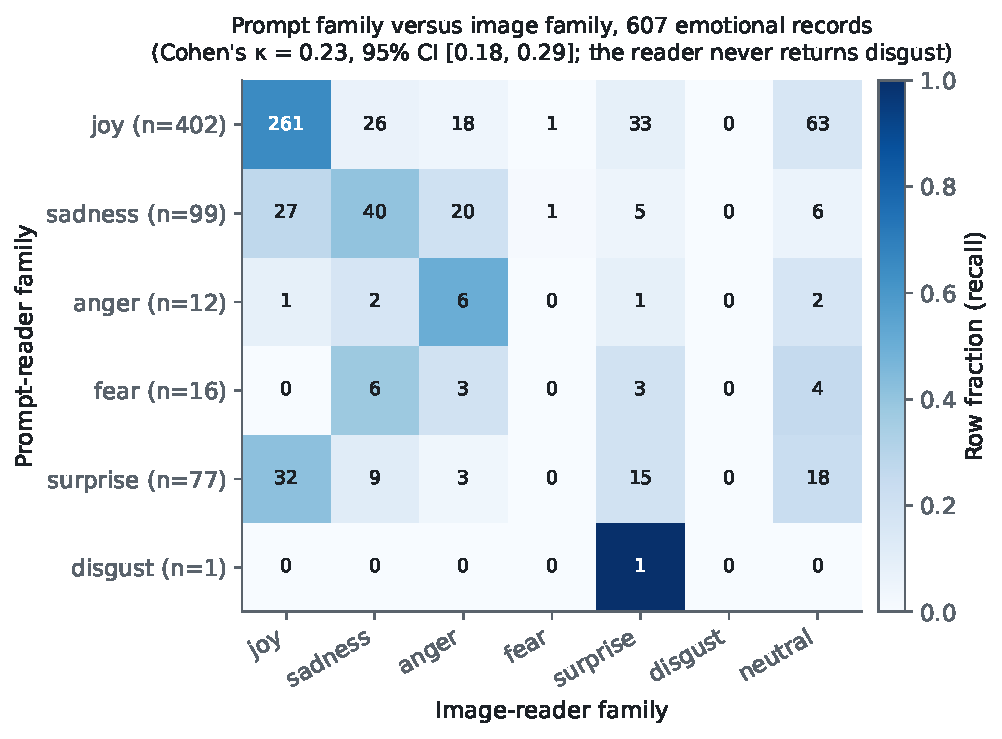
\includegraphics[width=0.85\textwidth]{fig6_confusion}
\caption{Prompt-reader family (rows) against image-reader family (columns) on the \nEmotional{} emotional records; cell = count, shading = row fraction.}
\label{fig:confusion}
\end{figure}

% GENERATED by emoviz/export_tex.py — do not edit
\begin{table}[htbp]
\centering
\scriptsize
\caption{Prompt-reader family (rows) against image-reader family (columns) on the 607 emotional records. Recall = row diagonal share, with a clustered-bootstrap 95\% CI. Cohen's $\kappa$ = 0.23 [0.18, 0.29]. The image reader never returns disgust and returns fear 4 times in 1,012 records.}
\label{tab:confusion}
\begin{tabular}{lrrrrrrrrl}
\toprule
Prompt \textbackslash{} image & joy & sadness & anger & fear & surprise & disgust & neutral & $n$ & Recall [CI] \\
\midrule
joy & 261 & 26 & 18 & 1 & 33 & 0 & 63 & 402 & 64.9\% [59, 70] \\
sadness & 27 & 40 & 20 & 1 & 5 & 0 & 6 & 99 & 40.4\% [31, 51] \\
anger & 1 & 2 & 6 & 0 & 1 & 0 & 2 & 12 & 50.0\% [22, 78] \\
fear & 0 & 6 & 3 & 0 & 3 & 0 & 4 & 16 & 0.0\% [0, 0] \\
surprise & 32 & 9 & 3 & 0 & 15 & 0 & 18 & 77 & 19.5\% [11, 28] \\
disgust & 0 & 0 & 0 & 0 & 1 & 0 & 0 & 1 & 0.0\% [0, 0] \\
\midrule
\textit{image total} & 321 & 83 & 50 & 2 & 58 & 0 & 93 & 607 &  \\
\bottomrule
\end{tabular}
\end{table}

% GENERATED by emoviz/export_tex.py — do not edit
\begin{table}[htbp]
\centering
\small
\caption{Cohen's $\kappa$ for family agreement (7 families), with clustered-bootstrap 95\% CIs and the Landis \& Koch (1977) band. The neutral-labelled subset is degenerate ($\kappa$ = 0 by construction) and is omitted.}
\label{tab:kappa}
\begin{tabular}{lrrll}
\toprule
Subset & $n$ & $\kappa$ & 95\% CI & Band \\
\midrule
emotional & 607 & 0.23 & [0.18, 0.29] & fair \\
face & 402 & 0.30 & [0.23, 0.37] & fair \\
scene & 205 & 0.13 & [0.06, 0.19] & slight \\
all analysed & 1012 & 0.21 & [0.16, 0.25] & fair \\
distinct emotional & 452 & 0.23 & [0.17, 0.29] & fair \\
distinct face & 319 & 0.29 & [0.21, 0.37] & fair \\
distinct scene & 133 & 0.09 & [0.01, 0.17] & slight \\
\bottomrule
\end{tabular}
\end{table}

% GENERATED by emoviz/export_tex.py — do not edit
\begin{table}[htbp]
\centering
\small
\caption{Top-1 family marginals of the two readers over all 1,012 analysed records.}
\label{tab:families}
\begin{tabular}{lrr}
\toprule
Family & Prompt reader & Image reader \\
\midrule
joy & 402 & 461 \\
sadness & 99 & 141 \\
anger & 12 & 89 \\
fear & 16 & 4 \\
surprise & 77 & 108 \\
disgust & 1 & 0 \\
neutral & 405 & 209 \\
\bottomrule
\end{tabular}
\end{table}


\section{The describer}
\label{sec:results-describer}

Table~\ref{tab:describer} crosses the describer's people count with the presence of an expression word over all \nAnalysed{} records. The describer answers the expression question for every drawing. It returns an expression word for \DescNoPeopleExpr{} of the records in which it simultaneously reports that no people are present. Of the \DescSceneN{} scene-classified records, \DescScenePeopleZero{} report no people; \DescScenePeopleZeroExpr{} of those still carry an expression word, and \DescSceneSmile{} answer ``smile'', ``smiling'' or ``happy'' (\DescSceneSmilePct{} of the no-people records). The smile rate depends on the denominator and is given with both: \DescSmileFace{} of the \nFaceAll{} face-classified records and \DescSmileAll{} of all \nAnalysed{} analysed records.

The copy rate measures how much the extraction stage adds to the describer's own word. Where the expression answer names an emotion outright (\DescBareStrictN{} records, \DescBareStrictPct{} of the corpus), the image reader's top-1 family equals the family that word implies \DescCopyStrict{} of the time. On the broad definition, which admits facial actions such as ``smile'' and ``crying'', the copy rate is \DescCopyBroad{}: \DescCopyBroadPeople{} where a person is reported and \DescCopyBroadPeopleZero{} where none is, the ``0 people'' token pulling the reading towards neutral.

% GENERATED by emoviz/export_tex.py — do not edit
\begin{table}[htbp]
\centering
\small
\caption{The describer's answers on all 1,012 analysed records: people count crossed with whether the facial-expression answer contains an expression word. The face rule is the top-left cell. Of the 421 scene-classified records, 414 report no people and 406 of those still contain an expression word (332 answer smile, smiling or happy).}
\label{tab:describer}
\begin{tabular}{lrr}
\toprule
 & Expression word present & Expression word absent \\
\midrule
People $\geq 1$ & 591 & 7 \\
People $= 0$ & 406 & 8 \\
\bottomrule
\end{tabular}
\end{table}


\section{Error taxonomy}
\label{sec:results-taxonomy}

\TaxN{} emotional records satisfy the high-confidence criterion, both readers scoring their top family at 0.8 or above and disagreeing; they cover \TaxDistinct{} distinct prompts, and since the count fell below the intended sample of 40, every one was examined. Figure~\ref{fig:taxonomy} and Table~\ref{tab:taxonomy} give the primary failure mode assigned from the drawing. By stage, \TaxDescriber{} of the \TaxN{} trace to the describer (\TaxA{} where it invented a face or an expression, \TaxB{} where it misread one), \TaxReader{} to the image reader inferring wrongly from a correct description, \TaxPrompt{} to the prompt side (\TaxD{} mixed or ambiguous prompts and \TaxF{} prompt-reader error), and \TaxGenerator{} to the drawing not depicting the prompt.

Two mechanisms stand out. A people count of zero predicts the invented-expression mode: \TaxPeopleZero{} of the \TaxN{} records carry that tag, and seven of the \TaxA{} invented-expression records do. And the joy-to-neutral cell is a single mechanism: prompts such as ``grateful'' and ``calm but tired'' describe low-arousal positive states for which the seven-family scheme has no home, the describer answers ``calm'' or ``smile'', and the reader returns neutral. Visitors also list feelings without connectives (``tired proud happy''), so the automatic tag for mixed prompts, which looked for ``but'' and ``although'', caught none of the eleven mixed-prompt records; a list detector would serve better.

\begin{figure}[htbp]
\centering
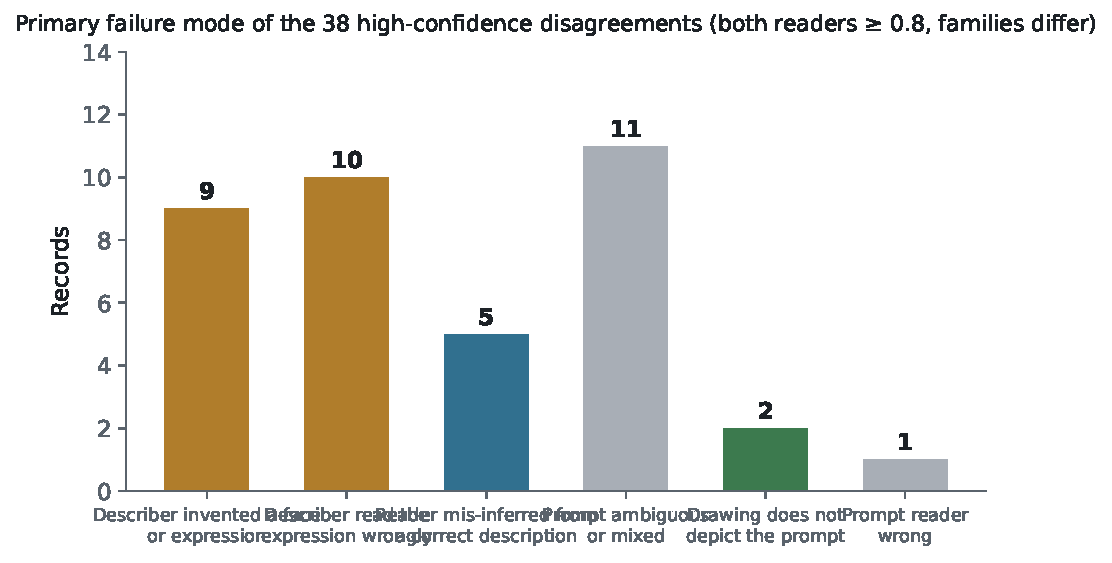
\includegraphics[width=0.95\textwidth]{fig7_error_taxonomy}
\caption{Primary failure mode of the \TaxN{} high-confidence disagreements, assigned from the drawing.}
\label{fig:taxonomy}
\end{figure}

% GENERATED by emoviz/export_tex.py — do not edit
\begin{table}[htbp]
\centering
\small
\caption{Primary failure mode of the 38 high-confidence disagreements (both readers' top-1 score $\geq 0.8$, families differ), assigned from the drawing. Describer faults (a+b) = 19; image reader (c) = 5; prompt side (d+f) = 12; generator (e) = 2.}
\label{tab:taxonomy}
\begin{tabular}{lp{0.55\textwidth}rl}
\toprule
Mode & Description & $n$ & Exemplar ids \\
\midrule
(a) & describer invented a face or expression where none is drawn & 9 & 18, 19, 242 \\
(b) & describer read the expression wrongly & 10 & 39, 192, 202 \\
(c) & reader mis-inferred from a correct description & 5 & 89, 107, 231 \\
(d) & prompt ambiguous or mixed & 11 & 65, 66, 93 \\
(e) & drawing does not depict the prompt & 2 & 137, 771 \\
(f) & prompt reader wrong & 1 & 436 \\
\bottomrule
\end{tabular}
\end{table}


\section{Description-template ablation}
\label{sec:results-ablation}

Table~\ref{tab:ablation} and Figure~\ref{fig:ablation} give the ladder under each altered template, with only the entailment stage re-run. The control re-run of the unmodified template reproduces the baseline exactly, changing the top-1 reading of \AblControlChanged{} records, so every difference in the table is a template effect and not numerical noise; the baseline row itself reproduces Section~\ref{sec:results-overall}.

Removing the expression sentence removes nearly all of the agreement. On the emotional prompts family agreement falls from \FullEmoFamObs{} to \AblDropExpressionEmoFamObs{} (null \AblDropExpressionEmoFamNull{}, $z$ = \AblDropExpressionEmoFamZ{}) and valence-sign agreement from \FullEmoSignObs{} to \AblDropExpressionEmoSignObs{} (null \AblDropExpressionEmoSignNull{}, $z$ = \AblDropExpressionEmoSignZ{}); on the face-classified records valence-sign agreement falls to \AblDropExpressionFaceSignObs{}. Fixing the expression word to ``unclear'' for every record produces the same collapse (family \AblFixedExpressionEmoFamObs{}, $z$ = \AblFixedExpressionEmoFamZ{}), and the reader's output under both variants falls to surprise or neutral for \AblDropExpressionSurprise{} and \AblDropExpressionNeutral{} of the \nAnalysed{} records respectively. Removing the action, posture or scene clause moves family agreement by one to three points (\AblDropActionEmoFamObs{}, \AblDropPostureEmoFamObs{}, \AblDropSceneEmoFamObs{}). Removing the people count raises rates and nulls together (scene valence-sign \AblDropPeopleSceneSignObs{} against \AblDropPeopleSceneSignNull{}, $z$ = \AblDropPeopleSceneSignZ{}): the ``0 people'' token pulls scene readings towards neutral, and without it the hallucinated smile is read as joy, which most prompts also are.

Under the people-aware template, which describes a drawing as ``A drawing showing \{scene\}.'' wherever the describer reports no people and leaves every other record unchanged, the face rows are identical to the baseline by construction (\AblPeopleAwareFaceSignObs{}, \AblPeopleAwareFaceFamObs{}) and the scene rows fall to their nulls: valence-sign agreement \AblPeopleAwareSceneSignObs{} against \AblPeopleAwareSceneSignNull{} ($z$ = \AblPeopleAwareSceneSignZ{}) and family agreement \AblPeopleAwareSceneFamObs{} against \AblPeopleAwareSceneFamNull{} ($z$ = \AblPeopleAwareSceneFamZ{}). Restoring the action and posture clauses to those records gives \AblPeopleAwareNoExpressionSceneSignObs{} against \AblPeopleAwareNoExpressionSceneSignNull{} ($z$ = \AblPeopleAwareNoExpressionSceneSignZ{}) and \AblPeopleAwareNoExpressionSceneFamObs{} against \AblPeopleAwareNoExpressionSceneFamNull{} ($z$ = \AblPeopleAwareNoExpressionSceneFamZ{}). Over all emotional prompts the people-aware template gives valence-sign agreement of \AblPeopleAwareEmoSignObs{} ($z$ = \AblPeopleAwareEmoSignZ{}) and family agreement of \AblPeopleAwareEmoFamObs{} ($z$ = \AblPeopleAwareEmoFamZ{}).

\begin{figure}[htbp]
\centering
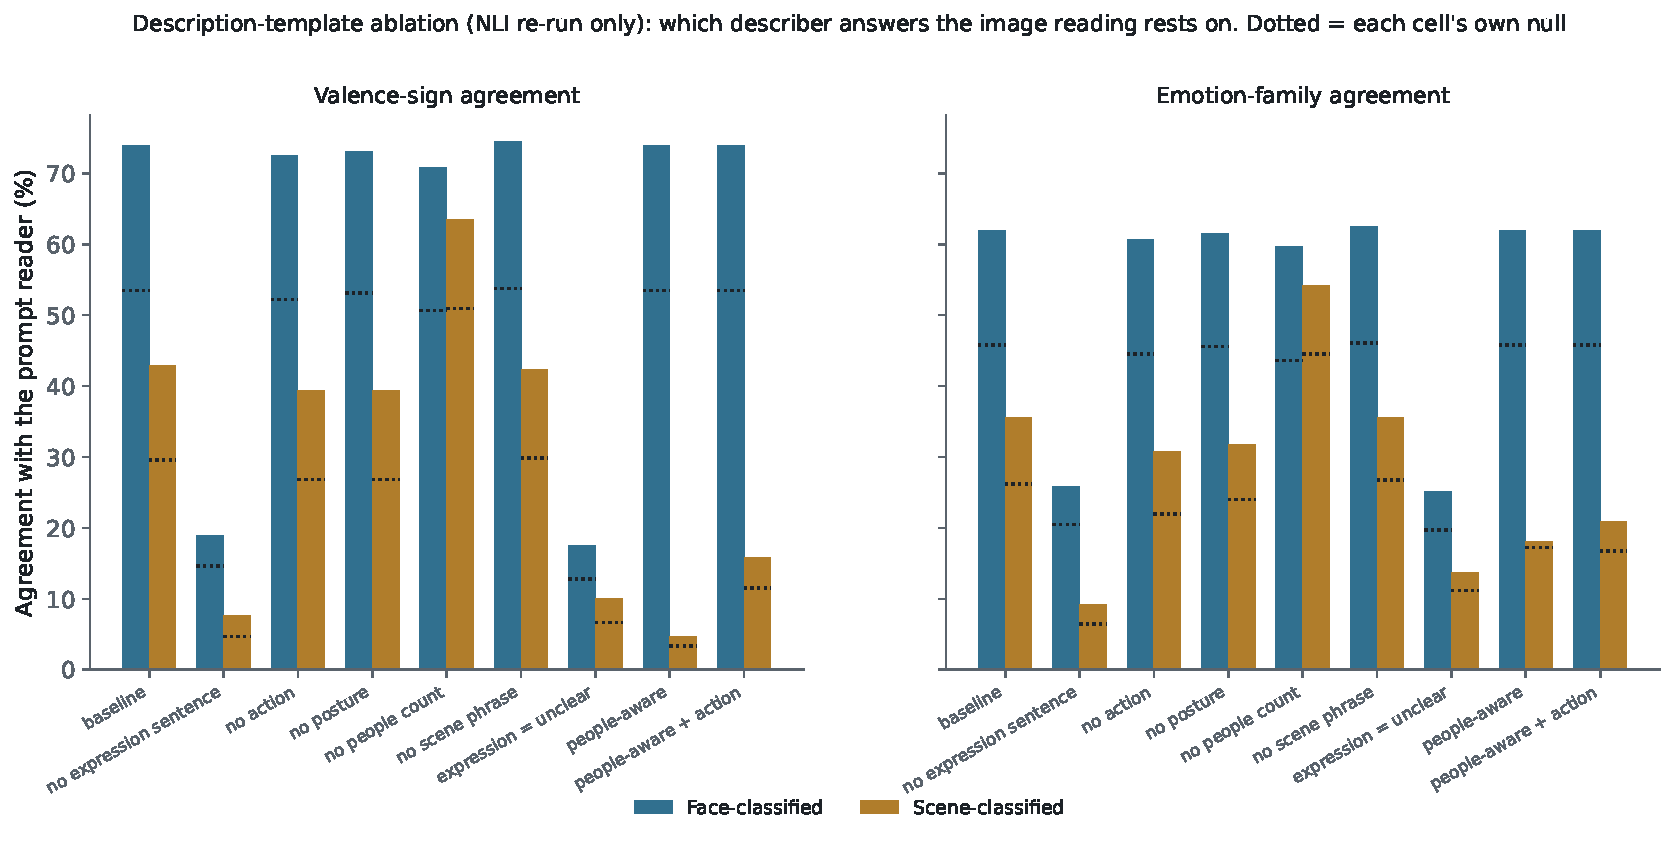
\includegraphics[width=\textwidth]{fig8_ablation}
\caption{Description-template ablation, with only the entailment stage re-run: valence-sign and family agreement by image class under each template, each bar against its own random-pairing null (dotted).}
\label{fig:ablation}
\end{figure}

% GENERATED by emoviz/export_tex.py — do not edit
\begin{table}[htbp]
\centering
\footnotesize
\caption{Description-template ablation: the NLI stage re-run on descriptions rebuilt from the cached describer answers with one clause removed or fixed; the prompt side and the null procedure unchanged. Valence-sign and family agreement per variant on the emotional prompts and their face/scene halves.}
\label{tab:ablation}
\begin{tabular}{llrrrrrrr}
\toprule
Variant & Subset & $n$ & Sign obs & null & $z$ & Family obs & null & $z$ \\
\midrule
baseline & emotional & 607 & 64.0\% & 45.6\% & +11.1 & 53.0\% & 38.8\% & +10.3 \\
 & face & 402 & 73.9\% & 53.5\% & +10.4 & 61.9\% & 45.8\% & +10.3 \\
 & scene & 205 & 42.9\% & 29.6\% & +5.8 & 35.6\% & 26.2\% & +4.4 \\
\midrule
drop\_expression & emotional & 607 & 15.3\% & 11.4\% & +5.1 & 20.3\% & 16.6\% & +3.8 \\
 & face & 402 & 18.9\% & 14.7\% & +3.8 & 25.9\% & 20.5\% & +3.8 \\
 & scene & 205 & 7.6\% & 4.7\% & +2.7 & 9.3\% & 6.4\% & +2.2 \\
\midrule
drop\_action & emotional & 607 & 61.9\% & 43.9\% & +11.0 & 50.6\% & 36.7\% & +10.3 \\
 & face & 402 & 72.5\% & 52.2\% & +10.4 & 60.7\% & 44.5\% & +10.4 \\
 & scene & 205 & 39.4\% & 26.8\% & +5.6 & 30.7\% & 21.9\% & +4.6 \\
\midrule
drop\_posture & emotional & 607 & 62.3\% & 44.5\% & +10.7 & 51.4\% & 37.9\% & +9.7 \\
 & face & 402 & 73.1\% & 53.1\% & +10.0 & 61.4\% & 45.6\% & +10.1 \\
 & scene & 205 & 39.4\% & 26.8\% & +5.6 & 31.7\% & 24.0\% & +3.6 \\
\midrule
drop\_people & emotional & 607 & 68.5\% & 50.7\% & +10.8 & 57.8\% & 43.7\% & +9.9 \\
 & face & 402 & 70.8\% & 50.7\% & +10.4 & 59.7\% & 43.6\% & +10.3 \\
 & scene & 205 & 63.5\% & 50.9\% & +5.0 & 54.1\% & 44.5\% & +3.8 \\
\midrule
drop\_scene & emotional & 607 & 64.2\% & 46.0\% & +10.7 & 53.4\% & 39.2\% & +9.8 \\
 & face & 402 & 74.4\% & 53.8\% & +10.4 & 62.4\% & 46.1\% & +10.1 \\
 & scene & 205 & 42.4\% & 29.9\% & +5.6 & 35.6\% & 26.8\% & +3.9 \\
\midrule
fixed\_expression & emotional & 607 & 15.1\% & 10.8\% & +5.9 & 21.3\% & 17.5\% & +3.9 \\
 & face & 402 & 17.5\% & 12.8\% & +4.4 & 25.1\% & 19.7\% & +4.0 \\
 & scene & 205 & 10.0\% & 6.6\% & +2.8 & 13.7\% & 11.2\% & +1.5 \\
\midrule
people\_aware & emotional & 607 & 51.7\% & 36.9\% & +10.1 & 47.1\% & 34.5\% & +8.8 \\
 & face & 402 & 73.9\% & 53.5\% & +10.4 & 61.9\% & 45.8\% & +10.3 \\
 & scene & 205 & 4.7\% & 3.4\% & +1.6 & 18.0\% & 17.3\% & +0.6 \\
\midrule
people\_aware\_no\_expression & emotional & 607 & 55.3\% & 39.5\% & +10.5 & 48.1\% & 35.0\% & +9.6 \\
 & face & 402 & 73.9\% & 53.5\% & +10.4 & 61.9\% & 45.8\% & +10.3 \\
 & scene & 205 & 15.9\% & 11.6\% & +2.7 & 21.0\% & 16.8\% & +2.2 \\
\midrule
control\_full\_template & emotional & 607 & 64.0\% & 45.6\% & +11.1 & 53.0\% & 38.8\% & +10.3 \\
 & face & 402 & 73.9\% & 53.5\% & +10.4 & 61.9\% & 45.8\% & +10.3 \\
 & scene & 205 & 42.9\% & 29.6\% & +5.8 & 35.6\% & 26.2\% & +4.4 \\
\bottomrule
\end{tabular}
\end{table}


\section{Single-coder reliability check}
\label{sec:results-human}

The 120-drawing sample has been drawn and laid out on six contact sheets (Figure~\ref{fig:codingsheet}); the coding was not complete at the time of writing, and the table in this section is generated from the scored file once it is. The table reports the describer's people count against the coder's, the face rule's precision and recall against the coder's face judgement, what lies behind the describer's ``smiling'' answers, the image reader's valence sign against the coder's, and the face/scene contrast recomputed on the coder's split rather than the describer's, which is the one estimate in the dissertation that breaks the circularity of Section~\ref{sec:method-pipeline} for the records it covers. It is a single coder, and it is stated as such.

% TODO once labels.csv is coded and `human_check.py score` has run: re-run export_tex.py, then replace this
% paragraph with the numbers (describer people-count agreement, face-rule precision/recall, smile precision,
% reader valence agreement with Wilson CIs, and the face/scene contrast on the coder's split).

% GENERATED — human check not scored when export_tex.py last ran; code outputs/human_check/labels.csv, run human_check.py score, then export_tex.py.
\noindent\emph{[Human-check table pending: code \texttt{outputs/human\_check/labels.csv}, run \texttt{human\_check.py score}, then \texttt{export\_tex.py}.]}


\section{Summary of findings}
\label{sec:results-summary}

\begin{enumerate}\setlength{\itemsep}{2pt}
\item On the \nEmotional{} prompts the text reader labels emotional, the two readers agree far above chance on every rung of the ladder: valence sign \FullEmoSignObs{} against \FullEmoSignNull{}, family \FullEmoFamObs{} against \FullEmoFamNull{}; the result survives clustering, the distinct-prompt re-run and the Holm correction (objectives 2 and 3).
\item Where the describer reports a readable face the agreement is far higher than where it reports a scene, by \DiffSignPp{} on valence sign (CI \DiffSignCi{}, $p$ = \DiffSignP{}); the scene result weakens on distinct prompts and, under a people-aware description, falls to its null (objectives 3, 4 and 7).
\item Prompts the text reader labels neutral sit at chance on the one measure that can move there, \CtrlVaObs{} against \CtrlVaNull{}, and remain there when the \CtrlFlagged{} prompts that contain an affect word are removed (objective 3).
\item Like for like, describe-then-extract agrees with the prompt reader on \McDeFam{} of families against \McClipFam{} for direct CLIP, a difference of \McDiffFamPp{} with $p$ \McClusterFamP{} on the clustered test (objective 5).
\item When the same words are drawn again, the image reader returns the same family for \ConsFam{} of drawings in a group against \ConsFamNull{} by chance ($z$ = \ConsFamZ{}): more consistent than chance and far from fixed (objective 6).
\end{enumerate}

The audits qualify all five. The describer names an expression for \DescScenePeopleZeroExpr{} of the \DescScenePeopleZero{} no-people scene records, the image reader copies an emotion-naming expression word \DescCopyStrict{} of the time, and the ablation shows that the reading rests on that word: the split and most of the agreement run through it.
   % Results
\chapter{Discussion}
\label{ch:discussion}

\section{What the results establish}
\label{sec:disc-establish}

Three things, and I want to be careful not to claim a fourth.

First, the emotion a text model recovers from a visitor's words and the emotion a second model recovers from the drawing made of those words agree far more often than chance would produce, on every rung of the ladder, and the effect is not an artefact of the things that most often produce artefacts in a corpus like this. It survives clustering on the prompt group, which takes the \nRepeats{} repeated records out of the count of independent evidence; it survives re-running on the first occurrence of every prompt; and it survives a Holm correction across every non-degenerate comparison the analysis prints. The valence-sign result, \FullEmoSignObs{} against \FullEmoSignNull{}, is the one I would defend in any room, because it asks the coarsest question and because its denominator is stated.

Second, the agreement is concentrated in drawings the describer reads as containing a face. Where it reports a scene, the agreement in the main table is weak, it weakens further on distinct prompts, and its family cell does not survive the multiplicity correction. The ablation then removes it: describe those drawings without the person and expression the template inserted, and this reader finds nothing above chance in them. That is a stronger statement than the one the project set out to make, and a different one. The design expected faces to agree more than scenes. What it found is that, for this instrument, faces agree and scenes do not.

Third, the instrument behaves as an instrument should on its checks. Prompts the text reader could not read affect from sit at chance on the one measure with a live null, and stay there when the prompts that plainly contain an affect word are removed. And, scored like for like, the describe-then-extract reader agrees with the prompt reader far more often than a direct CLIP reader does, by \McDiffFamPp{} on family with the clustered test at $p$ \McClusterFamP{}. That last result has to be framed with care. Neither image reader has ground truth. What the comparison shows is that two ways of reading a drawing disagree with each other on most records, and that one of them sits much closer to a third model's reading of the words. It does not show that either reader is more correct, and I have avoided the word throughout.

The fourth thing, the one not claimed, is any statement about what a person sees. Every number in this dissertation is the agreement of two machine readers. The human study that would turn agreement into perception is designed, its sample is drawn, and it is not done.

\section{The describer is the weak link}
\label{sec:disc-describer}

The audits were written to find out where the instrument bends, and they all point at the same place. The description template asserts a person and a facial expression for every drawing. The describer obliges: for \DescScenePeopleZero{} scene-classified drawings it reports that nobody is present and, in \DescScenePeopleZeroExpr{} of them, names an expression anyway, ``smile'', ``smiling'' or ``happy'' in \DescSceneSmile{} cases. The image reader then reads that sentence. Where the expression word names an emotion outright, which it does for \DescBareStrictPct{} of the corpus, the reader's top family is the family that word implies \DescCopyStrict{} of the time. The two-stage architecture was meant to keep the vision model away from the emotion judgement; the copy rate says that, for those records, the second stage relays the first.

The ablation says it more directly. Take the expression sentence out and family agreement on the emotional prompts falls from \FullEmoFamObs{} to \AblDropExpressionEmoFamObs{}; fix the expression word to ``unclear'' and it falls to \AblFixedExpressionEmoFamObs{}; take out any other clause and it moves by a point or three. The reading rests on one word. In effect the pipeline asks the describer what the face is doing and maps the answer to a family, with the entailment model as an expensive lookup table. That is a finding about the instrument rather than a failure of the project, and I would rather report it than have it found by an examiner, but it changes how the method comparison should be read: the advantage over direct CLIP may lie in BLIP-VQA being a better reader of drawn faces than CLIP is, not in the describe-then-extract architecture as such. An ablation that stripped emotion words from the expression answer before extraction would separate the two, and is listed as further work.

The error taxonomy closes the loop from the other direction. Of the \TaxN{} disagreements on which both readers were confident, \TaxDescriber{} trace to the describer, \TaxReader{} to the reader, \TaxPrompt{} to the prompt side and only \TaxGenerator{} to the drawing failing to depict the prompt. The generator, in other words, is rarely the reason the two readings differ; the readers are. This sits well with what the perception benchmarks report about vision--language models: a systematic bias towards positive labels \cite{bhattacharyya2025evaluating}, which appears here as a smile rate of \DescSmileFace{} on face-classified records and \DescSmileAll{} corpus-wide, and a confusion of what a subject expresses with what a viewer feels \cite{gao2025eemo}, which the describer's invented expressions are an extreme form of.

\section{Circularity of the face/scene split}
\label{sec:disc-circularity}

The face/scene split was my supervisor's hypothesis and the design's main contrast, and it needs its own paragraph of honesty. The split is defined from the describer's output: a person reported, and an expression word present. It is driven almost entirely by the people count, since \DescScenePeopleZero{} of the \DescSceneN{} scene-classified records are ones where the describer said nobody was there. The image reader then reads the same description. The contrast between the two classes is therefore a statement about the describer's output, not about faces in drawings, and it is entangled with its own definition. It is real in the sense that matters statistically: it clears its nulls, it survives clustering, and the permutation test puts it at $p$ = \DiffSignP{}. But what it establishes is that when the describer reports a face and an expression, the reader's family tracks the prompt, and when the describer reports no person, the reader has only an invented expression to go on and, once that is removed, nothing. Whether the scene drawings hold a feeling that a person can read is a question this design cannot answer, and the single-coder check, which classifies drawings without reference to the describer, is the only estimate in the project that can. Until it is scored, the right form of words is the one used in Chapter~\ref{ch:results}: faces, and only faces, for this reader.

\section{What is not claimed}
\label{sec:disc-not-claimed}

Four non-claims, each with its reason.

No direction between positive and negative feelings. The first build reported that negative feelings survived the drawing and positive ones collapsed; the second build, with a different image reader, reported the reverse. Both were wrong to report anything: within a single-valence subset the valence-sign null is degenerate, so there is nothing to test, and the raw difference on the loosest measure is a base-rate effect of where the families sit on the plane. Two readers that point in opposite directions cannot settle the question between them.

No statement about human perception. The word in the registered title is a question, not a result; the dissertation measures agreement between readers and says so on every page it can.

No claim about colour. The corpus is monochrome throughout and there is no colour condition. The colour literature \cite{alvarado2025texttoimage} explains why a monochrome corpus is a hard case, and that study models colour features only and is silent on line; nothing here can be attributed to the absence of colour rather than to the readers, the taxonomy or class rarity.

No claim about the generator alone from the consistency result. The \ConsFam{} within-group agreement against \ConsFamNull{} bounds the whole chain from prompt to reading. With no reliability estimate for the image reader, an unknown share of the variation is measurement noise, and with generation parameters unrecorded, the rest cannot be attributed to sampling rather than to prompt rewriting.

There is also a restriction rather than a non-claim. Fear (\RecFearN{} prompts), anger (\RecAngerN{}) and disgust (\RecDisgustN{}) are too rare on the prompt side to support a family-level statement, the image reader never returns disgust and returns fear \famImageFear{} times, and the surprise family is largely curiosity-mapped prompts under the standard label grouping. Claims are confined to overall agreement and the face/scene contrast.

\section{Relation to prior work}
\label{sec:disc-prior}

The closest study is Lomas and colleagues' human rating of emotional alignment for three generators \cite{lomas2024improved}. Their strongest secondary finding was that emotions rendered on a person aligned better than the same emotions rendered on a robot. The present project finds the same direction with machine readers and unmediated prompts, and then, through the ablation, finds that its own version of the effect is carried by a face being reported rather than by a face being drawn. The two results are consistent and neither validates the other, because theirs used human raters and templated prompts and this used machine readers and real ones; the human study that would connect them is the one the pipeline was built to precede.

The reasoning behind the ladder comes from Cowen and Keltner \cite{cowen2017self}: if experience is a set of categories bridged by gradients, near misses carry information. The results support the choice. Valence--arousal similarity and top-3 overlap both sit far above their nulls where family agreement is only \FullEmoFamObs{}, which says that the readers are close far more often than they coincide, and a right-or-wrong score would have called that closeness error.

The prompt reader's weakness on this register is the bound on everything downstream, exactly as the text literature predicts \cite{demszky2020goemotions, yang2023context}. A kappa of \KappaEmo{} on the emotional prompts, in the \KappaEmoBand{} band, is the kind of figure reported between human annotators for fine-grained emotion labelling of text, where GoEmotions' own raters agreed only moderately on many categories; two automatic readers separated by a generator and a drawing were never going to do better than the annotators of the training data did with each other. Carrasco and colleagues \cite{carrasco2024level} report that human agreement with a generator's emotion labels rises sharply once emotions are collapsed to positive and negative; the same pattern appears here in the gap between the valence-sign and family rungs.

The decision to read every value against a null follows Zhang and Wan \cite{zhang2025rethinking} and the holistic evaluation of Lee and colleagues \cite{lee2023holistic}, who show that automatic image--text scores move under trivial perturbations and correlate weakly with people. A score that changes its verdict under a one-pixel shift should not be quoted bare, and neither, this project argues, should a similarity whose floor is 0.41. Direct CLIP is the right baseline for the same reason CLIPScore \cite{hessel2021clipscore} is the field's default, and it fails here for the reason VQAScore's authors give for preferring a question-answering judge \cite{lin2024evaluating}: an embedding trained on captioned photographs has no purchase on a monochrome drawn face. The describer is, in that sense, a VQAScore-style judge pointed at expression rather than at objects, which is also why its expression answer does the work.

Finally, the positive bias the benchmarks find in vision--language models \cite{bhattacharyya2025evaluating} is reproduced here as a smile rate and as invented expressions, and WikiArt Emotions' observation that images with faces yield more consistent emotion judgements \cite{mohammad2018wikiart} is reproduced as the face/scene contrast, with the caveat that the consistency here is a machine's.

\section{Limitations}
\label{sec:disc-limitations}

\begin{enumerate}\setlength{\itemsep}{2pt}
\item There is no human anchor except the single-coder check, and that check is a single coder. Every result is reader-to-reader agreement.
\item The emotional/neutral split is the prompt reader's judgement, never human-checked; \CtrlFlaggedPct{} of the control contains an affect word, so the control is ``prompts the reader could not read affect from'' rather than ``prompts with no feeling''.
\item The face/scene split is circular: defined from the description the image reader reads, and driven by the people count.
\item The description template asserts a person and an expression for every drawing. Its consequence was measured, not designed away; a people-aware template is the obvious default for any future run.
\item Seven families have no home for low-arousal positive states, so ``calm'', ``grateful'' and ``at peace'' fall to neutral.
\item The family centroids are hand-placed; per-family means from the NRC norms \cite{mohammad2018obtaining} would replace a judgement with data.
\item The $z$-scores come from \nullShuffles{} re-pairings and are ordering statistics; across seeds the headline moves between \ZSeedMin{} and \ZSeedMax{}.
\item Generation parameters are unknown, so nothing can be regenerated and the consistency result cannot be decomposed.
\item Redaction leaves the drawing and the residual text in place, so re-identification risk is reduced, not removed.
\item One machine and one run: there is no second describer and no test--retest estimate for either reader.
\end{enumerate}

\section{Threats to validity}
\label{sec:disc-threats}

Construct validity is the governing threat: agreement between two readers is not affect as perceived, and the dissertation does not pretend otherwise. Internal validity is threatened by the leak from describer to reader and by the circular split, both of which are now quantified rather than assumed, and by pseudo-replication from repeated prompts, which the clustered inference addresses. External validity is limited to one generator, one festival, one language for the most part, and monochrome output; nothing here transfers to colour or to another model without being re-measured. Statistical validity is threatened by the number of comparisons, addressed by the Holm procedure, and by degenerate nulls, now detected from the null's own spread. The threats the design addressed are stated with the numbers that address them; the ones it could not address, above all the human anchor, are stated as the first items of further work.
   % Discussion
\chapter{Conclusions and Further Work}
\label{ch:conclusion}

% GUIDANCE (chapter target about 800 words). Summarise with acumen: what was asked, what was built,
% what was found, what it means, in that order — then further work that follows FROM the evaluation,
% not a wish list.

\section{Conclusions}
\label{sec:conc}
% GUIDANCE: Map back to the objectives in Section~\ref{sec:intro-aims}, one sentence each, with the
% deciding number as a macro (e.g. \FullEmoSignObs\ vs \FullEmoSignNull; \DiffSignPp; \McDiffFamPp;
% \ConsFam\ vs \ConsFamNull). End with the one-sentence answer to the question in
% Section~\ref{sec:intro-question}, bounded exactly as Section~\ref{sec:disc-not-claimed} bounds it.

\section{Further work}
\label{sec:further}
% GUIDANCE: In priority order, each tied to a limitation or an audit result:
%   1. A human-rated study of the drawings (the study this pipeline was built to precede), rating the
%      same ladder so machine and human agreement can be compared directly; \cite{lomas2024improved}
%      is the design to adapt.
%   2. A people-aware description template as the default (no expression clause when the describer
%      reports no people), with the demonstrator kept in parity; the ablation is its evidence.
%   3. A second describer (a sketch- or drawing-specific model was designed but not executed) and a
%      test--retest estimate for both readers, so the consistency result can be decomposed.
%   4. NRC-VAD per-family means in place of hand-set centroids \cite{mohammad2018obtaining}.
%   5. A richer family scheme (or the 27 categories of \cite{cowen2017self}) so low-arousal positive
%      states do not fall to neutral.
%   6. Extending the single-coder check to a second coder with an agreement statistic.
   % Conclusions and Further Work

\nocite{*}   % DRAFT ONLY: lists every bibliography entry so the .bib is checked. REMOVE before submission and cite what you use.
\bibliographystyle{acm}
\bibliography{mybibliography}

\begin{appendices}
\chapter{Reproducibility}
\label{app:repro}

% Factual listing; no prose needed beyond a sentence introducing each list.
\begin{sloppypar}

\section{Repository layout}
\begin{itemize}\setlength{\itemsep}{1pt}
\item \texttt{emoviz/emoviz/metrics.py} --- the single definition of every measure, split rule, centroid and the random-pairing null; imported by every script.
\item \texttt{emoviz/emoviz/data.py} --- the loader: filename schemes, timestamps, prompt groups, name redaction at load time.
\item \texttt{emoviz/preprocess\_names.py} --- the three-stage redaction procedure; the decision table travels with the dataset.
\item \texttt{emoviz/describe\_extract.py} --- the pipeline (BLIP-VQA $\to$ template $\to$ BART-MNLI); crash-safe, resumable.
\item \texttt{emoviz/analysis\_final.py} --- splits, ladder, nulls, distinct-prompt re-run; writes \texttt{outputs/analysis\_final.json}.
\item \texttt{emoviz/significance.py} --- clustered bootstrap and clustered permutation test of the face/scene difference.
\item \texttt{emoviz/inference.py} --- clustered CIs for every subset, Cohen's $\kappa$, Holm--Bonferroni, seed stability.
\item \texttt{emoviz/method\_comparison.py} --- like-for-like image-reader comparison with paired tests.
\item \texttt{emoviz/data\_audit\_consistency.py} --- data accounting and the repeated-prompt consistency with its permutation null.
\item \texttt{emoviz/audits.py} --- control contamination, describer leak and copy rate, per-family recall.
\item \texttt{emoviz/error\_taxonomy.py} --- the high-confidence disagreement census and failure modes.
\item \texttt{emoviz/ablate\_nli.py} --- description-template ablation (NLI stage only).
\item \texttt{emoviz/human\_check.py} --- the single-coder sample, contact sheets and scoring.
\item \texttt{emoviz/make\_figures.py} and \texttt{emoviz/export\_tex.py} --- every figure and every number in this document, generated from the JSON result files.
\item \texttt{emoviz/app.py} and \texttt{emoviz/web/} --- the demonstrator.
\item \texttt{emoviz/test.sh} and \texttt{emoviz/test\_numeric.py} --- the smoke suite and the pinned numeric checks.
\item \texttt{emoviz/outputs/} --- cached model outputs, result JSON, figures, the frozen direct-CLIP baseline.
\end{itemize}

\section{Run order}
\begin{enumerate}\setlength{\itemsep}{1pt}
\item \texttt{bash emoviz/setup.sh} --- creates the environment from the pinned \texttt{requirements.txt}.
\item \texttt{describe\_extract.py} --- the pipeline over all images (cached; re-run only to regenerate).
\item \texttt{analysis\_final.py} --- the main analysis (seconds; uses the cached outputs).
\item \texttt{significance.py}, \texttt{inference.py}, \texttt{method\_comparison.py}
\item \texttt{data\_audit\_consistency.py}, \texttt{audits.py}, \texttt{error\_taxonomy.py}, \texttt{ablate\_nli.py}
\item \texttt{human\_check.py sample}; code \texttt{outputs/human\_check/labels.csv}; \texttt{human\_check.py score}
\item \texttt{make\_figures.py}; \texttt{export\_tex.py}; then build this document (\texttt{pdflatex}, \texttt{bibtex}, \texttt{pdflatex} twice).
\item \texttt{bash emoviz/test.sh} --- runs everything above that is fast, plus \texttt{test\_numeric.py}.
\end{enumerate}
All scripts are run with \texttt{emoviz/.venv/bin/python} from the \texttt{emoviz/} directory.

\section{Environment}
% GUIDANCE: Python 3.12; torch, transformers and open\_clip versions from requirements.txt; Apple MPS
% in float16 for the models; models and their parameter counts: Salesforce/blip-vqa-base,
% facebook/bart-large-mnli, SamLowe/roberta-base-go\_emotions, OpenCLIP ViT-B/32; total download
% about 3.5 GB; the pipeline processed \nTotal\ images with no unhandled error (a robustness
% statement, not a correctness one).

\end{sloppypar}
  % Reproducibility
\chapter{Instruments}
\label{app:instruments}

\section{The five describer questions}
The describer is asked, in this order, and its answers are stored per record:
\begin{enumerate}\setlength{\itemsep}{1pt}
\item \emph{What is the facial expression?} (\texttt{expression})
\item \emph{What is the person doing?} (\texttt{action})
\item \emph{What is the body posture?} (\texttt{posture})
\item \emph{How many people are there?} (\texttt{people})
\item \emph{What is in the picture?} (\texttt{scene})
\end{enumerate}
The word ``emotion'' appears in none of them.

\section{The description template}
The five answers are composed into one sentence:
\begin{quote}\ttfamily
A drawing of \{people\} showing \{scene\}. The person is \{action\}, \{posture\}. The facial expression is \{expression\}.
\end{quote}
The template is applied to every record, including those where \texttt{people} is ``0'' or ``none''; the ablation variants remove one clause at a time or fix \texttt{expression} to ``unclear''.

\section{The image reader's hypothesis}
Zero-shot classification by entailment with the hypothesis template
\begin{quote}\ttfamily
This scene conveys \{family\}.
\end{quote}
scored for each of the seven families; the three highest entailment scores are kept.

\section{GoEmotions labels to families}
\begin{description}\setlength{\itemsep}{1pt}
\item[joy] admiration, amusement, approval, caring, desire, excitement, gratitude, joy, love, optimism, pride, relief
\item[sadness] disappointment, embarrassment, grief, remorse, sadness
\item[anger] anger, annoyance, disapproval
\item[fear] fear, nervousness
\item[surprise] surprise, realization, confusion, curiosity
\item[disgust] disgust
\item[neutral] neutral
\end{description}
Family scores are the sums of the member probabilities, normalised to a distribution.

\section{Family centroids on the circumplex}
\begin{center}
\begin{tabular}{lrr}
\toprule
Family & Valence & Arousal \\
\midrule
joy & $+0.80$ & $0.60$ \\
sadness & $-0.75$ & $0.30$ \\
anger & $-0.70$ & $0.80$ \\
fear & $-0.65$ & $0.75$ \\
surprise & $+0.30$ & $0.80$ \\
disgust & $-0.70$ & $0.60$ \\
neutral & $0.00$ & $0.30$ \\
\bottomrule
\end{tabular}
\end{center}
Hand-set from the standard placement of the basic emotions on the circumplex; the minimum of Eq.~\ref{eq:va} over these points is $0.412$.

\section{Readable expression words}
A record is face-classified when the describer reports at least one person and its expression answer contains one of:
\begin{quote}
smile, smiling, happy, sad, angry, serious, surprised, surprise, calm, excited, crying, laughing, frowning, scared, shocked, worried, concentration, concentrating, grin, grinning, neutral, confused, determined, pensive, sleepy, sleeping.
\end{quote}
The people count is parsed from digits or number words (none, one, two, \dots, several, many, crowd, group, lots); a non-empty answer that is neither is read as one person present.

\section{Name redaction procedure}
\begin{enumerate}\setlength{\itemsep}{1pt}
\item \textbf{Detect.} Candidates from three detectors: a given-name gazetteer (7,944 names), mid-sentence capitalised tokens absent from a 236k-word English dictionary, and naming phrases (``called X'', ``my friend X''). High recall by design, because most prompts are written entirely in lower case.
\item \textbf{Review.} Every candidate has a recorded decision (redact or keep) with a reason and, for redactions, the record it applies to. The audit fails if any candidate is unreviewed or if a redaction entry matches nothing.
\item \textbf{Apply.} At load time, per record, replacing the token with \texttt{[name]}; consecutive placeholders collapse to one. The files on disk are never modified. Illness, grief and place names are kept.
\end{enumerate}

\section{Single-coder check: coding instructions}
The coder works from numbered contact sheets that show only the drawings, and fills four columns per drawing:
\begin{description}\setlength{\itemsep}{1pt}
\item[person] y / n --- is at least one person or face drawn?
\item[face] y / n --- is there a face whose expression can be read? (n if no person)
\item[valence] $+$ / $-$ / 0 --- the feeling the drawing gives: positive, negative, neither
\item[family] joy / sadness / anger / fear / surprise / disgust / neutral
\end{description}
The sample is fixed by seed (120 drawings: 40 face-classified, 40 scene-classified with no people reported, and every record with a vague or word-only people answer, topped up equally from the first two strata). The prompt, the description and the model readings are not shown during coding.
  % Instruments
\end{appendices}

\end{document}
